\documentclass[british,titlepage,table,xcdraw]{ntnuthesis}

\title{Face Image Quality}
\shorttitle{Face Image Quality}
\author{Walid Demloj, Hans Petter Fauchald Taralrud, Kjetil Grosberghaugen, Julian Nyland Skattum}
\shortauthor{W. Demloj, H. P. F. Taralrud, K. Grosberghaugen, J. N. Skattum }
\date{CC-BY \ntnuthesisdate}

\addbibresource{thesis.bib}
\usepackage{float} % added by Walid 
\usepackage{multirow} % added by Walid 



% From https://www.overleaf.com/learn/latex/Glossaries

\makeglossaries % Prepare for adding glossary entries


\newglossaryentry{latex}
{
        name=latex,
        description={Is a mark up language specially suited for
scientific documents}
}

\newglossaryentry{bibliography}
{
        name=bibliography,
        plural=bibliographies,
        description={A list of the books referred to in a scholarly work,
typically printed as an appendix}
}

\newglossaryentry{maths}
{
    name=mathematics,
    description={Mathematics is what mathematicians do}
}

% Words to define
%scrum
%frontend
%backend
%api
%dataset
%kanban
%biometric
%REST / RESTful
%sprint
%use case
%Github
%repository
%React.js
%Node.js
%Axios
%web framework? Explain what it is
%Docker
%Containerization / containers
%dockerfiles
%biometric
%Telegram

% --------------------
% ----- Acronyms -----
% --------------------
\setglossarypreamble[acronym]{The page number after an acronym refers to the first time it is used in the thesis.}
\newacronym{api}{API}{Application Programming Interface}
\newacronym{ai}{AI}{artificial intelligence}
\newacronym{cie}{CIE}{International Commission on Illumination}
\newacronym{cnn}{CNN}{Convolutional Neural Network}
\newacronym{covid19}{COVID-19}{Coronavirus disease 2019}
%\newacronym{csv}{CSV}{Comma-separated values}
\newacronym{cvd}{CVD}{Colour Vision Deficiency}
\newacronym{dom}{DOM}{Document Object Model}
\newacronym{xml}{XML}{Extensible Markup Language}
\newacronym{xhtml}{XHTML}{Extensible HyperText Markup Language}
\newacronym{xp}{XP}{Extreme Programming}
\newacronym{fiqm}{FIQM}{Face Image Quality Metric}
\newacronym{fiqa}{FIQA}{Face Image Quality Assessment}
\newacronym{fr}{FR}{Face Recognition}
\newacronym{gdpr}{GDPR}{General Data Protection Regulation}
\newacronym{html}{HTML}{HyperText Markup Language}
\newacronym{http}{HTTP}{Hypertext Transfer Protocol}
\newacronym{icao}{ICAO}{International Civil Aviation Organization}
\newacronym{iec}{IEC}{International Electrotechnical Commission}
\newacronym{iso}{ISO}{International Organization for Standardization}
\newacronym{json}{JSON}{JavaScript Object Notation}
\newacronym{mrtd}{MRTD}{Machine Readable Travel Documents}
\newacronym{mvc}{MVC}{Model-View-Controller}
\newacronym{mtcnn}{MTCNN}{Multitask Cascaded Convolutional Networks}
\newacronym{ntnu}{NTNU}{Norwegian University of Science and Technology}
%\newacronym{ux}{UX}{User Experience}
%\newacronym{ui}{UI}{User Interface}


 % add glossary and acronym lists before document

\begin{document}

\chapter*{Abstract}

The performance of face recognition systems are dependent on images used for training and analysis. There are metrics that automatically can calculate the quality of the images. In this project we have evaluated two face image quality metrics provided by Mobai. The project consisted of creating a web application that automates the process of evaluating datasets and that can easily add new FIQMs into the application. We are also comparing the scores provided by the FIQMs with human assessments by arranging a subjective experiment to collect ground truth data. 


The performance of face recognition systems are dependent on images used for training and analysis. There are metrics that automatically can calculate the quality of images. In this project we have evaluated two face image quality metrics provided by Mobai. The project consisted of creating a web application that evaluates images by the use of different Face Imaqe Quality Metrics (FIQM). We have also conducted a subjective experiment to collect ground truth data on three datasets Mobai gave us and compared them with the scores from the FIQMs to see the correlation. Further, we have expanded the task by creating our own dataset consisting of new aspects and distortions, and conducted a new subjective experiment. The subjective results from this dataset has then been used to correlate with the two FIQMs.

\chapter*{Sammendrag}
Ytelsen på ansiktgjenkjenningssystmer er avhengig av kvaliteten på bildene for å kunne teste og trene disse systemene. For å automatisk vurdere kvaliteten på ansiktsbilder blir Face Image Quality Metrics (FIQMs) benyttet. Slike kvalitetsmetrikker gir objektive resultater som korresponderer med hvor synlig ansiktet i et bilde er. I dette prosjektet introduserer vi en webapplikasjon som regner ut slike objektive resultater med to moderne FIQMs. For å vurdere nøyaktigheten på disse metrikkene, samlet vi inn subjektive data fra eksperter og ikke-eksperter på tre forskjellige dataset. Vi samlet også inn et nytt dataset med ansiktsbilder som vi mener er overlegent i forhold til andre nåværende dataset. Denne overlegenheten er med tanke på antall bilder, type forvregninger bildene er påvirket av og hvordan bildet er tatt (bilder med ansiktsmasker og bilder med skrå vinkler). Resultatene viser at de objektive resultatene regnet ut av de to kvalitetsmetrikkene har lav korrelasjon med de subjektive resultatene samlet inn via subjektive eksperimenter. 


\tableofcontents
\listoffigures
\listoftables
\lstlistoflistings

\glsaddall
\printglossary[type=\acronymtype] % Print acronyms
%\printglossary                    % Print glossary

\chapter{Introduction}
\label{chap:Intro}

\section{Background}
\label{section:background}
Mobai is a spin off company from the research developed in the Norwegian Biometrics Laboratory at the \acrfull{ntnu}. They provide solutions for facial recognition, biometrical attack detection and face morph detection. To create models for detection of biometrical attributes, artificial intelligence \acrshort{ai} and machine learning are essential tools for Mobai. In addition to the models, having access to appropriate datasets plays a crucial role in training and developing new models. An important focus of Mobai is using different \acrlong{fiqm}s (\acrshort{fiqm}s) to determine the quality of facial images in a dataset. In order to train models, quickly assess several datasets or create new datasets, it is important to know the quality of facial images. Therefore, Mobai now aims to develop an application that automates this process. 

\section{Subject Area}
Digital image processing is a rapidly growing field within the world of engineering and computer science. A great amount of research has been done in this field of study, paving the way for multimedia systems to become one of the pillars of the modern information society. Digital image processing is used in a variety of technologies, including face detection and face recognition which itself could be categorized under the broader field of patter recognition. Digitalization has drastically changed peoples everyday lives over the last decade, and with that change, biometrics has become more relevant and important than ever. 

Solutions such as face recognition, presentation attack detection and face morph detection all heavily rely on the quality of the facial images used for machine learning training. The quality of facial images are dependent on several factors which FIQMs have learned trough artificial intelligence and machine learning. FIQMs' performance can be measured by comparing the quality scores with human assessment. This thesis is mainly focused on Face Image Quality Assessment (\acrshort{fiqa}) which plays a key role in improving the accuracy of face recognition systems. 

\section{Task Description}
\label{sec:TaskD}
This bachelor project can be divided into two main parts, a programming part (mainly Chapter \ref{chap:objective}) and a research part (mainly Chapter \ref{chap:subjective}).

\subsection*{Programming}
The programming part involves the creation of an application that uses two FIQMs provided by Mobai for evaluating the quality of facial images. The application will create a report which contains the FIQM calculations in the set of images. The key functionalities of the application expected from Mobai are: 
\begin{itemize}
    \item The user should be able to read/select images from a local machine.
    \item The user should be able to upload images to a directory.
    \item The user should be able to execute the two FIQMs on the uploaded images.
    \item The user should be able to display the results from the FIQMs. 
\end{itemize}

\subsection*{Research}
The research part consists of conducting a subjective experiment. The subjective experiment involves collecting ground truth data by having subjects evaluate the quality of facial images from a dataset based on certain criteria. During the experiment, observers will be shown different facial images of varying quality and asked to label the images into predefined categories. The subjective results will then be used to compare with the objective results from the FIQMs. By comparing the subjective results from the experiment with the objective measure calculated by FIQMs we are then able to evaluate the performance of FIQMs. 

\section{Delimitation}
\label{sec:delimit}
In this project, our task was not solely made up of pure programming. Fortunately, the subject field we were working within allowed research which we found to be a great experience in the final step of our bachelor studies. As an example, facial images used for research in the field of face quality assessment and face recognition were usually taken from a straight angle with little to no tilting of the camera lens. After a literature review it was evident that studies addressing camera tilting was very limited. With the ongoing pandemic, wearing face masks in public has become a habit. Even though wearing a mask is a new aspect of our daily lives, the performance of FIQMs on images which show a subject wearing a face mask has not yet been studied. In that case, we wanted to assess the performance of the FIQMs on face mask images. For the mentioned reasons, the bachelor group proposed the collection of a new dataset which Mobai supported the initiative. The mentioned dataset will not only be used by Mobai in their studies but can also be used by the bachelor group. Further information about the collected dataset is provided in Section \ref{sec:ownData}. Finally we should point out that with the exception of our dataset, all FIQMs and datasets were provided to the bachelor group by Mobai. 

\section{Target Groups}
\label{sec:TargetGroups}
In general, this project is targeted towards two groups, Mobai and the readers of the thesis. 

\subsection{Users of the Web Application}
The web application will be used by employees at Mobai to evaluate the performance of the FIQMs on different datasets. Based on the Non Disclosure Agreement (NDA) signed by the bachelor group (Appendix \ref{app:project-agreements}), because of possible competitive companies neither the source code or the application should be distributed to others except Mobai.

\subsection{Thesis Readers}
The target group for the bachelor thesis are people who need insight in how we did the project from a developer point of view as well as a scientific point of view. This includes but is not limited to our thesis supervisor, client and fellow students with similar background that can be interested in reading the thesis.

\section{The Team}
In this section we will introduce the members in our team. Here we look at their interests, responsibilities and their academic backgrounds. 

\subsection{The Members}

\subsubsection*{Hans Petter}
Hans Petter is a computer engineer who is interested in mathematics and artificial intelligence. He is interested in Python programming and was therefore one of the main developers of the backend. Hans Petter had the main responsibility for implementing \acrshort{api}s to the frontend. He also helped out the other team members whenever there were any API errors connecting Flask to React or general Python problems. In addition to the application task, Hans Petter collected the data from the subjective experiment to make it workable. 

\subsubsection*{Walid}
Walid has prior knowledge with artificial intelligence and finds topics that mix statistics and mathematics with artificial intelligence interesting. Throughout the project, Walid was mainly involved in the creation of the backend logic with Hans Petter. In particular, he developed API endpoints used by the frontend. 

\subsection*{Julian}
Julian is a computer engineer with an interest in programming, mathematics and artificial intelligence. His background consists of different subjects regarding programming, mathematics, software security and application development. Julian's main responsibility was creating the frontend of the application and handling the data received by the backend. 

\subsubsection*{Kjetil}
Kjetil is a developer with an interest in front end web-development, JavaScript and Python programming. Due to his background and interests, his main responsibility was to work with the frontend and help with the backend development. 


\subsection{Academic Background}
\label{section:academic background}
All group members are studying for a bachelor´s degree in computer engineering, hence our academic backgrounds are closely similar. However, during the fifth semester, we all chose different subjects. Hans Petter and Walid both chose \textit{artificial intelligence}, \textit{software design} and \textit{calculus 3}. Julian had the elective subjects \textit{application development}, \textit{software security} and \textit{calculus 3}, while Kjetil studied the subjects: \textit{ergonomics in digital media}, \textit{infrastructure as code} and \textit{application development}. 

Throughout our bachelor´s program we have acquired a solid foundation when it comes to the software development process and scientific thinking by finishing courses like \textit{software engineering}, \textit{algorithmic methods}, \textit{operating systems}, \textit{scientific computing}, \textit{calculus} and \textit{physics}. The compulsory courses we finished helped us see different approaches to the same problem. There will always be several ways to approach a task and a bachelor´s degree in computer engineering has cemented that statement. Our prior knowledge made it easier to understand and process the main concepts of the new topics we had to learn. 

During this semester, we have acquired more knowledge and built on our foundation. We had to perform research on specific topics in backend and frontend programming, as these were topics we were unfamiliar with. More specifically, the part of connecting the frontend to the backend by using API calls, was something we had never done before. In addition to that, a high amount of time was also spent on learning how to conduct and perform scientific experiments in a way that satisfies both \acrfull{gdpr} and the relevant \acrshort{iso}-standards.  

\section{Why Did We Choose This Task?}
Although stationed in Gjøvik the group had never heard of Mobai or what they do. Their task description seemed interesting, and we were early to contact them. Already at the first meeting, before any bachelor tasks were selected, we got a very positive impression. The participants from Mobai were very curious and enthusiastic. They had clear ideas and suggestions on how we could approach the task. After this meeting, the bachelor thesis choice became an easy decision. 

A reason why we chose this task was the field of work. All group members were interested in machine learning and artificial intelligence. Therefore, we saw the topic as a perfect opportunity to have a hands on experience working in this field. Another reason for our choice was the width of the project. We felt that we could use experiences and knowledge learned throughout the bachelor courses in this work. We had to combine math, statistics and programming with research, which given our bachelor's program suited us well. This kind of scope was complex, but manageable, and challenged us in several ways in terms of coding and research. We were motivated by the fact that Mobai expected us to create an application that they would utilize in addition to creating a subjective experiment.   

\subsection{Roles}
\label{subsec:roles}
Our project work areas were mainly divided into two categories: research and programming. While studying FIQMs, the subjective assessment and the creation of a subjective experiment which can be seen as research were done collectively to ensure equal professional foundation. When it came to the programming part, each group member were delegated responsibility more individually. However, due to the nature of the work, we had to closely collaborate with each other with backend and frontend because its dependency. During the project, the following roles were assigned to each group member:
\begin{itemize}
    \item Kjetil Grosberghaugen was scrum master and developer. His main responsibility was frontend, written in React.js. As a scrum master he ensured the development process flew evenly and led sprint meetings.
    \item Julian Nyland Skattum was a developer with main responsibility in frontend. He was also responsible for programming language choices as well as the overall application appearance. 
    \item Hans Petter Fauchald Taralrud was a developer with main responsibility\\ in backend. 
    \item Walid Demloj was a developer with main responsibility in backend. 
\end{itemize}

Every member were participating in the full stack application despite their area of responsibility. The reason for having individual responsibilities was to easily maintain that the requirements were met. The group members had joint responsibility for the project plan (see Appendix \ref{app:project-plan}) and thesis as well as completing tasks according to the created requirements. 

Seyed Ali Amirshahi was our supervisor. The project group had scheduled meetings every Monday at 12:00. Ali's role in the project was to guide us throughout the project. He would evaluate the project plan, thesis and answer professional questions. Summaries of the meetings with Ali be found in Appendix \ref{appendix:supervisor}.

Kjartan Mikkelsen started as the product owner, but after about three months in the process, he left the company. Our new product owner and contact was Guoqiang Li. He expressed Mobai's vision and wishes during the project. We also got technical assistance from other employees at Mobai. Summaries of the meetings with Mobai can be found in Appendix \ref{appendix:Mobai}.

\subsection{Decision Making}
The group decided to go for a collaborative decision-making \cite{GroupDecisionMaking} approach when making choices throughout the project. Decisions like frontend and backend environment and experiment platform were decided collectively with knowledge and experience in mind. A touch of prior knowledge benefited our project, so we did not need to learn everything from scratch. Making choices in groups led to a comfortable team atmosphere with a good relationship between each team member. The decentralization of decision responsibilities made it easier to contribute in the decision making, because possible failures would be shared in the group. However, if a discussion had reached an impasse, the group leader had the final say. Choices related to project work were brought up in the daily scrum meetings, as they offered frequent changes as well as a cordial environment to give feedback and improvements. Choices related to project organization was arranged in the sprint retrospective meetings, every other week. 


\section{Thesis Structure}
It is important to emphasize that this thesis is atypical. As almost every bachelor task include reporting the development process, our thesis adds an extra dimension in terms of research. The subjective part requires thorough research to be able to correctly compare with the results provided by the application. All this are reflected in the way we structured our thesis. 
We have chosen to structure the thesis as follows: in Chapter \ref{chap:Specification}, we are discussing our choice of development methodology. We look at pros and cons for the methodology, address other possible development methods and elaborate the current development layout. Following the chosen development approach is an in-depth risk analysis. Chapter \ref{chap:FQA} is an important part of the thesis. Here we define some of the most essential concepts used in the project. We describe the definition of a good facial image in face recognition as well as introducing the FIQMs used in the application. Next, in Chapter \ref{chap:objective} we will look at how the face image metric application has been implemented and the reasoning behind our choices. In Chapter \ref{chap:subjective} we go through the process of conducting a subjective experiment to gather ground truth data. We also introduce the datasets used in the experiment and explain our own dataset creation. 
Both the objective assessment and subjective experiments are merged together in the results Chapter \ref{chap:Results}, where their results are compared. Following the results, we can conclude the FIQMs strengths and weaknesses based on their correlation with the subjective scores. In the conclusion Chapter \ref{chap:Conclusion} we conclude the results and introduce further work based on our research. The reasoning behind this project structure is mainly to provide the thesis readers a clear overview and a sequential story. Since the project's contents of the work are split, it is meaningful to describe the workload in separate chapters. 
\chapter{Specification}
\label{chap:Specification}
In this chapter we will start by looking at our chosen development method for the project and obstacles that arose with it. To end the chapter of, an in depth risk analysis will be presented.


\section{Development method}
Projects of this size are dependant on well structured development methods to succeed as it affects the way teams are organized and tasks are delegated. The prioritization of workload is also affected with the choice of development method. 
This project was characterised by uncertainty, a limited amount of labor and a development phase with requirements that may change. These characteristics paved the way for us to pick an agile software development method which was suggested by our client Mobai.  
\begin{enumerate}
    \item \textbf{Constant feedback} 
    
    \hspace{0,5cm}Our group consists of four third year students with little to none experience with comprehensive projects of this size. Such lack of experience alone causes some uncertainty in regards to deadlines, survey work and development. Having regular meetings with both Mobai and our project supervisor as well as receiving regular feedback, will decrease the chance to drift of track. This also ensures that our final product is as close to Mobai's vision as possible. Agile software development methods provides the client with the chance to be far more involved in the project. This aspect itself was an important point to take into consideration.
        
    \item \textbf{Small team}
    
    \hspace{0,5cm}For a team like us, an agile method is more suited because small teams are better positioned to efficiently and effectively manage events like meetings \cite{SmallTeams}. The reduction of communication channels in a team decreases the possibility of misinterpretations among members. A small team is more likely to have an attentive communication where decisions are made quickly.
    \newpage
    
    \item \textbf{All known requirements are not final}
    
    \hspace{0,5cm}In agile development methods it is expected that all the requirements are not finalized or even known in advance. Throughout the development process new requirements may be added and existing ones can be refined to better suit the upcoming application. This agility is not achieved by plan driven approaches because all requirements must be finalized in the planning phase. Bachelor projects rarely turn out exactly as planned, which is why an agile development method that handles changes would be beneficial. 
\end{enumerate}

\subsection{Considered models}
Although the scale tipped towards an agile methodology, we also included plan-driven approaches in our considerations in case they were a better solution. Following is our reasoning behind considered models.  

\subsubsection*{Waterfall method}
The fundamental process activities is broken down into linear sequential pha-ses\cite{WaterfallMethod}. Each phase has to be completed before it cascades into the next. This allows for departmentalization and control where deadlines can be set for every phase, resulting in a clear workflow. However, this model would not be suitable for our development due to its lack of revision. Should the development phase run into issues that was not taken into consideration in the planning or design phase, the design phase would have to start over. This would be very time consuming. Also, not having a working product until late in the development life cycle would be risky in regards to our programming uncertainty.   

\subsubsection*{Extreme Programming}
Extreme Programming (XP) emphasises five key values: communication, feedback, simplicity, courage and respect. It strives for high team efficiency and higher quality code by implementing 12 practises such as, refactoring, pair programming, test first development, continuous integration and simple design. Programmers are expected to work closely together, which is encouraged by the values mentioned \cite{eXtremeP}. The main downside however, is its strict and difficult way of working. It requires great self discipline to follow all the practises the method is built upon. XP mainly focuses on how software development should be approached, and since our project was not solely based on development, the model did not seem to fit our needs.  
\newpage

\subsubsection*{Kanban}
Kanban provides solid structuring and flexibility. The methodology is all about limiting work in progress as well as maximizing the work efficiency. It is based on a continuous workflow structure with continuous deliveries with no set dates. This ensures the team is ready to adapt to change whenever priorities may change. The kanban team are reliant on each other to succeed. No predefined roles are set, which means it is a collective responsibility of the team to work together and finish tasks. Likewise, no set dates are placed for when certain functionality should be released \cite{kanban}. We felt that this ``go with the flow'' mentality of kanban would lead to more uncertainty regarding the bachelor groups progress. The roles and responsibilities structuring of kanban, reinforced this mindset.  

\subsubsection*{Scrum}
Scrum is adjustable, flexible and a fast agile method that largely involves the client throughout the project cycle\cite{ScrumDefinition}. The requirements are never entirely determined which allows for updating the product. Small teams with defined roles are appropriate to provide different responsibility within the team. Having regular meetings ensures good communication as well as keeping team members up to date with the continuous progress.    

\subsection{Our model}
\label{sec:OurModel}
We chose to use a scrum model for this project. In addition, we wanted to implement the pair programming practise from XP since it would help to produce high-quality code as well as share experience in the field of programming. The pair programming was executed by screen sharing or with Visual Studio Code live-share. We also wanted to easily manage our working tasks. Therefore, we applied a kanban board to get a clear overview of the tasks that needed to be done. Trello \cite{Trello} was used for tracking the tasks and the tasks were divided into three phases: To-Do, Doing and Done. Since Kanban was not our main method, no specific rules or limitations were set considering the amount of tasks in each phase. Due to the project's nature, the adaptability and flexibility provided by scrum seemed to be a safe option which could also increase the chances of success in the project. The way the model organizes workload into different sprints and facilitates to pre-defined member roles helped us to keep up with the progression made throughout the project. Should we finish Mobai's desired application quickly it was suggested by Mobai that additional functionality could be added to the solution if our time schedule allowed for it. Changes in requirements were something Mobai were open to discuss and scrum handles this well, which was another reason for our choice. 

\subsection{Scrum layout}
We had sprints with a two-week duration. This is because, one-week sprints felt short and would lead to excessive meetings which would affect our time management. Longer sprints however, tend to involve the client to a lesser degree, which would not be ideal in our case. The involvement of the client was not only to have continues feedback to ensure that we satisfied their requirements, but it was what Mobai had emphasized on at the start of the project. The sprints consisted of several meetings and scrum practises, such as Sprint planning meetings, Daily scrums, Sprint review meetings and Sprint retrospective meetings. These meetings were all followed to a certain extent. 

\subsubsection*{Sprint planning meeting}
The start of the sprints took place on Tuesdays, (with the first meeting on the 2\textsuperscript{nd} of February) and were expected to finish by 11:00 every other Monday. The weekly scheduled meetings with our bachelor supervisor took place every Monday at 12:00, which gave us at least one hour to prepare both the next sprint and what we should discuss during the meeting. This is when all our sprint planning meetings were held and conversations about what features should be included in the upcoming sprint were planned. \textit{Planning poker} was used to estimate the time spent on different tasks.

\subsubsection*{Daily scrum}
These short meetings were held at the start of every day at 9:00 and were included to assure the members were kept up to date about the progress of the project.

\subsubsection*{Sprint review meeting}
The sprint review meetings with Mobai were arranged every other Tuesday, at the end of each sprint. Mobai was informed about our progress and provided us feedback. While these meetings were mainly attended by the product owner (Dr. Guoqiang Li) who provided feedback from the client's side, other employees of Mobai also attended these meetings. 

\subsubsection*{Sprint retrospective meeting}
At the end of each sprint right after our sprint review meetings with Mobai, time was delegated into the sprint retrospective meetings. During these meetings we reflected about what had went well and tried to improve these aspects for the next sprints. A crucial part of these meetings was to decide if our time estimates were on point. 

\subsubsection{Definition of done}
We used the scrum-pattern Definition of done \cite{DoneDone} to collectively define what development-tasks were considered done. In partnership with Mobai we came to an agreement upon different criteria that form the definition of done. It was important to set different criteria to different work tasks (there should be a difference between coding-criteria and report-criteria). This pattern gave us a familiar understanding of work quality and absoluteness. We also obtained good habits in our workflow using the definition of done as a checklist to correlate with the user stories. In that way we prevented possible delays occurring in the development process. Here is an example of our report-criteria: 

\begin{enumerate}
    \item The section is completed according to the member.
    \item The member has analyzed the section's contents.
    \item The section is checked for typos.
    \item The whole group has read and approved the section.
\end{enumerate}

\subsection{Difficulties with our model}
At the early stages of planning our bachelor project, our own development method seemed to fit all our requirements and needs with few disadvantages. However, once the development began, we quickly realised specific elements that were not desirable. 

Our pair programming practise inspired by XP did not work out as we intended or predicted it would. As it in the initial start of the project was very helpful to share experience, later in the development process, we came to the realization that it was very time consuming and limiting. Originally, the pair programming was supposed to be done on Visual Studio Code's Live Share, which allows developers to collaborate in real-time. However, the Live Share platform was constantly lagging for some of the members, which was why we decided to achieve pair programming by screen-sharing instead. This method forced one member to write code while the other observed and gave input which we found out to be unproductive and a waste of our limited resources. Because of that, we ended up coding the product mostly individually. The quality of the code was likely affected by this, however the productivity of the team became increasingly higher. The progress was easily traceable given our everyday meetings on online platforms.   

All meetings associated with scrum presented in the end of the previous section were beyond doubt time consuming and required certain planning in advance. The planning poker time estimating game was abandoned after a while because we felt it took valuable time away from the project. At the start it was a great tool that served us quite well, but as the project became clearer, we developed an understanding of time estimates. Because of that, we ended up estimating tasks verbally, which saved us time and resources.  

\section{Risk analysis} 
Almost every decision made throughout the project involved a risk. A risk was made up by the likelihood of something going wrong and the negative conse-quences entailed with that risk. Therefore, weighing up the risks before making a decision was very important. The better we understood occurring risks, the more we were prepared to manage them. Carrying out a risk analysis was beneficial for us to make sure every decision were robust and well considered. Our risk identification was done by discussing possible events that could occur, as well as identifying their likelihood and consequences. Prior knowledge from earlier projects helped us estimate whether a risk was likely or unlikely to happen. Since we were working agile, not all risks were decided in advance, but some were appended along the project process. The team categorized the risks according to the type of risk. The risk categories we used were: Project, Product and Business, which had been discussed in  detail \cite{RiskAnalysis}. 

\begin{itemize}
    \item \textbf{Project risks} 
        \par \hspace{0,5cm} Risks that affect available resources assigned to the project. These risks interfere with the schedule and may hinder reaching planned deadlines. 
    \item \textbf{Product risks} 
        \par \hspace{0,5cm} Risks that affect the overall performance of the system created. Risks in this category may affect the functionality which can reduce the overall quality. 
    \item \textbf{Business risks}
        \par \hspace{0,5cm} These risks affect the organization developing of a product. During this project, such risks will mainly be related to the team members as well as collaborators such as Mobai and our supervisor. 
\end{itemize}

Each risk listed below in the section, was evaluated and assessed based on its consequence and likelihood (Table\ref{table:colorC}). The numbers inside the Table reference what the risks were, and have nothing to do with the priority or severity. 
    
\begin{itemize}
    \item \textbf{Risk 1:} Group members leaving the project.
    \item \textbf{Risk 2:} Sprint deadlines are not met.
    \item \textbf{Risk 3:} Bachelor thesis is not finished in time.
    \item \textbf{Risk 4:} Mobai´s expected involvement turn out to be minimal. 
    \item \textbf{Risk 5:} A similar product launches.
    \item \textbf{Risk 6:} The software does not fulfill the minimum requirements.
    \item \textbf{Risk 7:} Inadequate planning and execution of subjective experiment.
    \item \textbf{Risk 8:} Loss of vital documents or source code.
    \item \textbf{Risk 9:} Sickness among group members, project supervisor or employees at Mobai.
    \item \textbf{Risk 10:} Application breaking bugs.
    \item \textbf{Risk 11:} Planned tools for development of the survey and application prove to be unsatisfactory. 
    \item \textbf{Risk 12:} Covid-19 restrictions interfere with the subjective experiment. 
    \item \textbf{Risk 13:} Unable of connecting the frontend to the backend logic. 
    \item \textbf{Risk 14:} Unrealistic demands are made along the way by the Product Ow-ner. 
    \item \textbf{Risk 15:} Additional help is required by other group members to overcome a specific problem.
\end{itemize}

\begin{table}[h]
\caption{Consequence and likelihood color coding risk matrix}
\label{table:colorC}
\resizebox{\textwidth}{!}{%
\begin{tabular}{ll|l|l|l|l|}
\cline{3-6}
 &
  \textbf{} &
  \multicolumn{4}{c|}{\textbf{Consequence}} \\ \cline{3-6} 
 &
  \multicolumn{1}{c|}{} &
  \cellcolor[HTML]{C0C0C0}{\color[HTML]{333333} Minor} &
  \cellcolor[HTML]{C0C0C0}{\color[HTML]{333333} Moderate} &
  \cellcolor[HTML]{C0C0C0}{\color[HTML]{333333} Major} &
  \cellcolor[HTML]{C0C0C0}{\color[HTML]{333333} Critical} \\ \hline
\multicolumn{1}{|l|}{} &
  \cellcolor[HTML]{C0C0C0}Unlikely &
  \cellcolor[HTML]{32CB00} R5 &
  \cellcolor[HTML]{32CB00} &
  \cellcolor[HTML]{F8FF00} R1 \& R4 \& R6 &
  \cellcolor[HTML]{FE0000} R3 \& R8 \& R13 \\ \cline{2-6} 
\multicolumn{1}{|l|}{} &
  \cellcolor[HTML]{C0C0C0}Likely &
  \cellcolor[HTML]{32CB00} R14 &
  \cellcolor[HTML]{F8FF00} R11 &
  \cellcolor[HTML]{F8FF00} R2 &
  \cellcolor[HTML]{FE0000} R10 \\ \cline{2-6} 
\multicolumn{1}{|l|}{} &
  \cellcolor[HTML]{C0C0C0}Quite likely &
  \cellcolor[HTML]{F8FF00} R15 &
  \cellcolor[HTML]{F8FF00} &
  \cellcolor[HTML]{FE0000} R7 \& R9 {\color[HTML]{FFFFFF} } &
  \cellcolor[HTML]{FE0000} \\ \cline{2-6} 
\multicolumn{1}{|l|}{\multirow{-4}{*}{\rotatebox[origin=c]{90}{\textbf{Likelihood}}}} &
  \cellcolor[HTML]{C0C0C0}Very likely &
  \cellcolor[HTML]{F8FF00} &
  \cellcolor[HTML]{FE0000} R12 &
  \cellcolor[HTML]{FE0000}{\color[HTML]{FFFFFF} } &
  \cellcolor[HTML]{FE0000} \\ \hline
\end{tabular}%
}
\end{table}

Table \ref{table:colorC} showcases a standard consequence/likelihood risk ranking matrix split into the likelihood of a risk occurring, and its corresponding consequence (i.e severity). The consequences ranges from minor to critical and the likelihood from unlikely to very likely. The three colors represent different type of risk levels. The green color indicates low risk, yellow indicated moderate risk and red represent risks of great importance. 

We chose a $4\times4$ matrix with three color codes because it covers and classifies a wide specter of risks. We could have settled for a $3\times3$ matrix, but we felt that risks would overlap and therefore a more severe risk could be mixed with a risk with lesser severity. Although a $5\times5$ matrix could have also be used, but since our project was limited in size relative to corporate projects, we felt that this type of granularity was not needed. 

In the next pages, all the above mentioned risks are placed into the three categories presented, and discussed with countermeasures. 

\begin{table}[h]
\caption{Project risks}
\resizebox{\textwidth}{!}{%
\begin{tabular}{|l|p{4cm}|p{7cm}|}
\hline
\rowcolor[HTML]{C0C0C0} 
\textbf{ID}                 & \textbf{Description} & \textbf{Countermeasures} \\ \hline
\cellcolor[HTML]{FE0000}R3  &    
Bachelor thesis is not finished in time. 
&
Base our time estimates on worst-case scenarios, that way if tasks are finished before a set date, some extra time can be added to the end for polishing purposes.
\\ \hline
\cellcolor[HTML]{FE0000}R7  &    
Inadequate planning and execution of subjective experiment. 
& 
Creating the survey at an early stage and studying the pitfalls in conducting surveys will minimize the risk of designing a lackluster and confusing survey. For more in depth and specific countermeasures, see Section \ref{sec:ConductingSurvey} Conducting the survey. 
\\ \hline
\cellcolor[HTML]{FE0000}R8  &      
Loss of vital documents or source code. 
& 
Using backup-technologies when writing the report and coding the software prevents loss of important content. The thesis will be synced with a GitHub repository and changes to the Overleaf project will regularly be pushed to the repository. 
\\ \hline
\cellcolor[HTML]{FE0000}R12 &      
Covid-19 restrictions interfere with the subjective experiment. &
It is highly likely that we won´t be able to conduct the experiment in a controlled environment which may affect subjects image evaluations. An instruction manual will be provided to all participants. 
\\ \hline
\cellcolor[HTML]{F8FF00}R2  &     
Sprint deadlines are not met. 
&      
Having a consistent workflow and a regular meeting schedule, makes it easier to meet the deadlines. If there are too many tasks in the upcoming sprint, a rescheduling may occur and the Product Owner will be informed. 
\\ \hline
\cellcolor[HTML]{F8FF00}R4  &      
Mobai´s expected involvement turn out to be minimal. 
&
Doing a lot of early research about our subject field is important to understand the basics, which we can build on ourselves. In addition, our supervisor should be utilized as best as possible.
\\ \hline
\cellcolor[HTML]{F8FF00}R15 &        
Additional help is required by other group members to overcome a specific problem. &
Our research and planning should make us capable of knowing a little about several topics. Members should therefore be able to assist each other if needed.
\\ \hline
\end{tabular}%
}
\end{table}


\begin{table}[h]
\caption{Product risks}
\resizebox{\textwidth}{!}{%
\begin{tabular}{|l|p{4cm}|p{7cm}|}
\hline
\rowcolor[HTML]{C0C0C0} 
\textbf{ID}                 & \textbf{Description} & \textbf{Countermeasures} \\ \hline
\cellcolor[HTML]{FE0000}R10 &
Application breaking bugs. 
& 
Analyze what critical bugs can occur when developing the product at an early stage. Applying continuous testing throughout the development phase should mitigate large faults in the application. 
\\ \hline
\cellcolor[HTML]{FE0000}R13 &
We are unable to connect the frontend to the backend logic.  
&
We should minimize the use of hard coding that may interfere with connecting React to Flask. Additionally, study materials which could help us in this issue should be studies by the members. Lastly, Mobai´s development team may assist us if needed. 
\\ \hline
\cellcolor[HTML]{F8FF00}R6  &
The software does not fulfill the minimal requirements. 
&  
Keeping a consistent workflow insures maximum efficiency. Should problems, which forces us to exceed deadlines by a great margin occur, a meeting with Mobai will be held where the requirements should be reconsidered. 
\\ \hline
\cellcolor[HTML]{F8FF00}R11 &
Planned tools for development of the survey and application prove to be unsatisfactory. 
& 
All tools should be replaceable and carefully considered through research to minimize the use of inefficient tools. Most of our requirements should be met by the tool. If several tools match our needs, the most suitable and quickest to learn will be chosen.  
\\ \hline
\end{tabular}%
}
\end{table}

\begin{table}[h]
\caption{Business risks}
\resizebox{\textwidth}{!}{%
\begin{tabular}{|l|p{4cm}|p{7cm}|}
\hline
\rowcolor[HTML]{C0C0C0} 
\textbf{ID}                 & \textbf{Description} & \textbf{Countermeasures} \\ \hline 
\cellcolor[HTML]{FE0000}R9  &
Sickness among group members, project supervisor or Mobai. 
&
The team shall follow the regional and local Covid-19 measures to the greatest extent. Members becoming ill should be kept up to date about the progress of the project. Additionally, to prevent rescheduling, members should know what the rest of the group is working on. Daily meetings will be an effective countermeasure. 
\\ \hline
\cellcolor[HTML]{F8FF00}R1  &
Group members leaving the project. 
&  
A structured group with good planning and communication reduces the risk of members leaving the project. A safe team atmosphere where members are encouraged to bring fourth new ideas and input is essential. The team members should also be given the opportunity to work with something they find interesting and fun. Should however a member leave the team, a redistribution of the remaining work tasks shall be equally split amongst the remaining members. 
\\ \hline
\cellcolor[HTML]{32CB00}R5  &
A similar product launches. 
&
If a similar product launches, it is important to meet all of Mobai´s specialized needs and avoid delays in the deployment. 
\\ \hline
\cellcolor[HTML]{32CB00}R14 &
Unrealistic demands are made along the way by the Product Owner. 
&
Our agile development method will mitigate large reschedules of the project if new demands are provided. However, our main task is written in the task description (\ref{sec:TaskD}) and any additional demands are not required by us to complete. 
\\ \hline
\end{tabular}%
}
\end{table}



\chapter{Face Quality Assessment}
\label{chap:FQA}

\section{What is a good image?}
\label{sec:setup}
Throughout this thesis we will mention the word quality several times. While some people already have a good understanding of what the word means, some confusion may arise. 

Within the standard image quality assessment field, the definition of quality is straight forward and is what most people think about when hearing the word. Ordinary people and people working with images will for the most part think about the image resolution as the most important characteristic that defines image quality. An excellent image of a face with this definition would have high resolution and sharp focus.   

However Mobai´s and our definition differs from the usual way image quality is defined. Our emphasis lies not with the image resolution itself, but with how well the face is visible. There are several aspects that heavily affect the quality of facial images with respect to biometric systems performance. These aspects are presented and discussed in two important papers: 

\begin{itemize}
    \item ISO/IEC TR 29794-5:2010: Information technology — Biometric sample quality — Part 5: Face image data \cite{ISO50912}.
    \item ICAO Doc 9303 Part 3: Specifications Common to all MRTDs \cite{ICAO1}. 
\end{itemize}

The quality specific aspects of facial images presented in the two standards are what defines the quality in our thesis. The different quality factors are:  

\begin{itemize}
    \item Scenery characteristics like lighting or background.
    \item Characteristics like the consistency between the skin colour on the image and the skin colour of the subject.
    \item Complete or partial face coverings.
    \begin{itemize}
        \item Glasses fully covering the eyes.
        \item Any type of head coverings.
    \end{itemize}
    \item The behaviour of the subject.
    \begin{itemize}
        \item Closed or open eyes.
        \item Closed or open mouth.
        \item Any kind of expression, e.g. smiling or neutral.
        \item Head pose, e.g. frontal or rotated in any direction.
    \end{itemize}
    \item Image properties like the size of the image or its resolution.
    \item Image appearance characteristics like the exposure or noise.
\end{itemize}

The above mentioned aspects all affect the quality of the facial image to some degree. What we consider an excellent facial image is similar to a standard passport image with the following characteristics: 
\begin{itemize}
    \item Open and visible eyes.
    \item No dark tinted glasses. 
    \item Neutral or little to none facial expression.
    \item Neutral head pose.
    \item No garments covering the face.
    \item Clean background.
    \item Neither too dark or too light.
    \item Photo taken neither too close or too far away.
\end{itemize}

The characteristics will affect the quality in a good or bad way. If all the bullet points above are true, the quality of the facial image is near perfect. An image of a half-covered or missing face will negatively affect the quality, even though the image resolution itself may be impeccable. 

\begin{figure}[h]
\centering
    \subfloat[Excellent facial image]
        {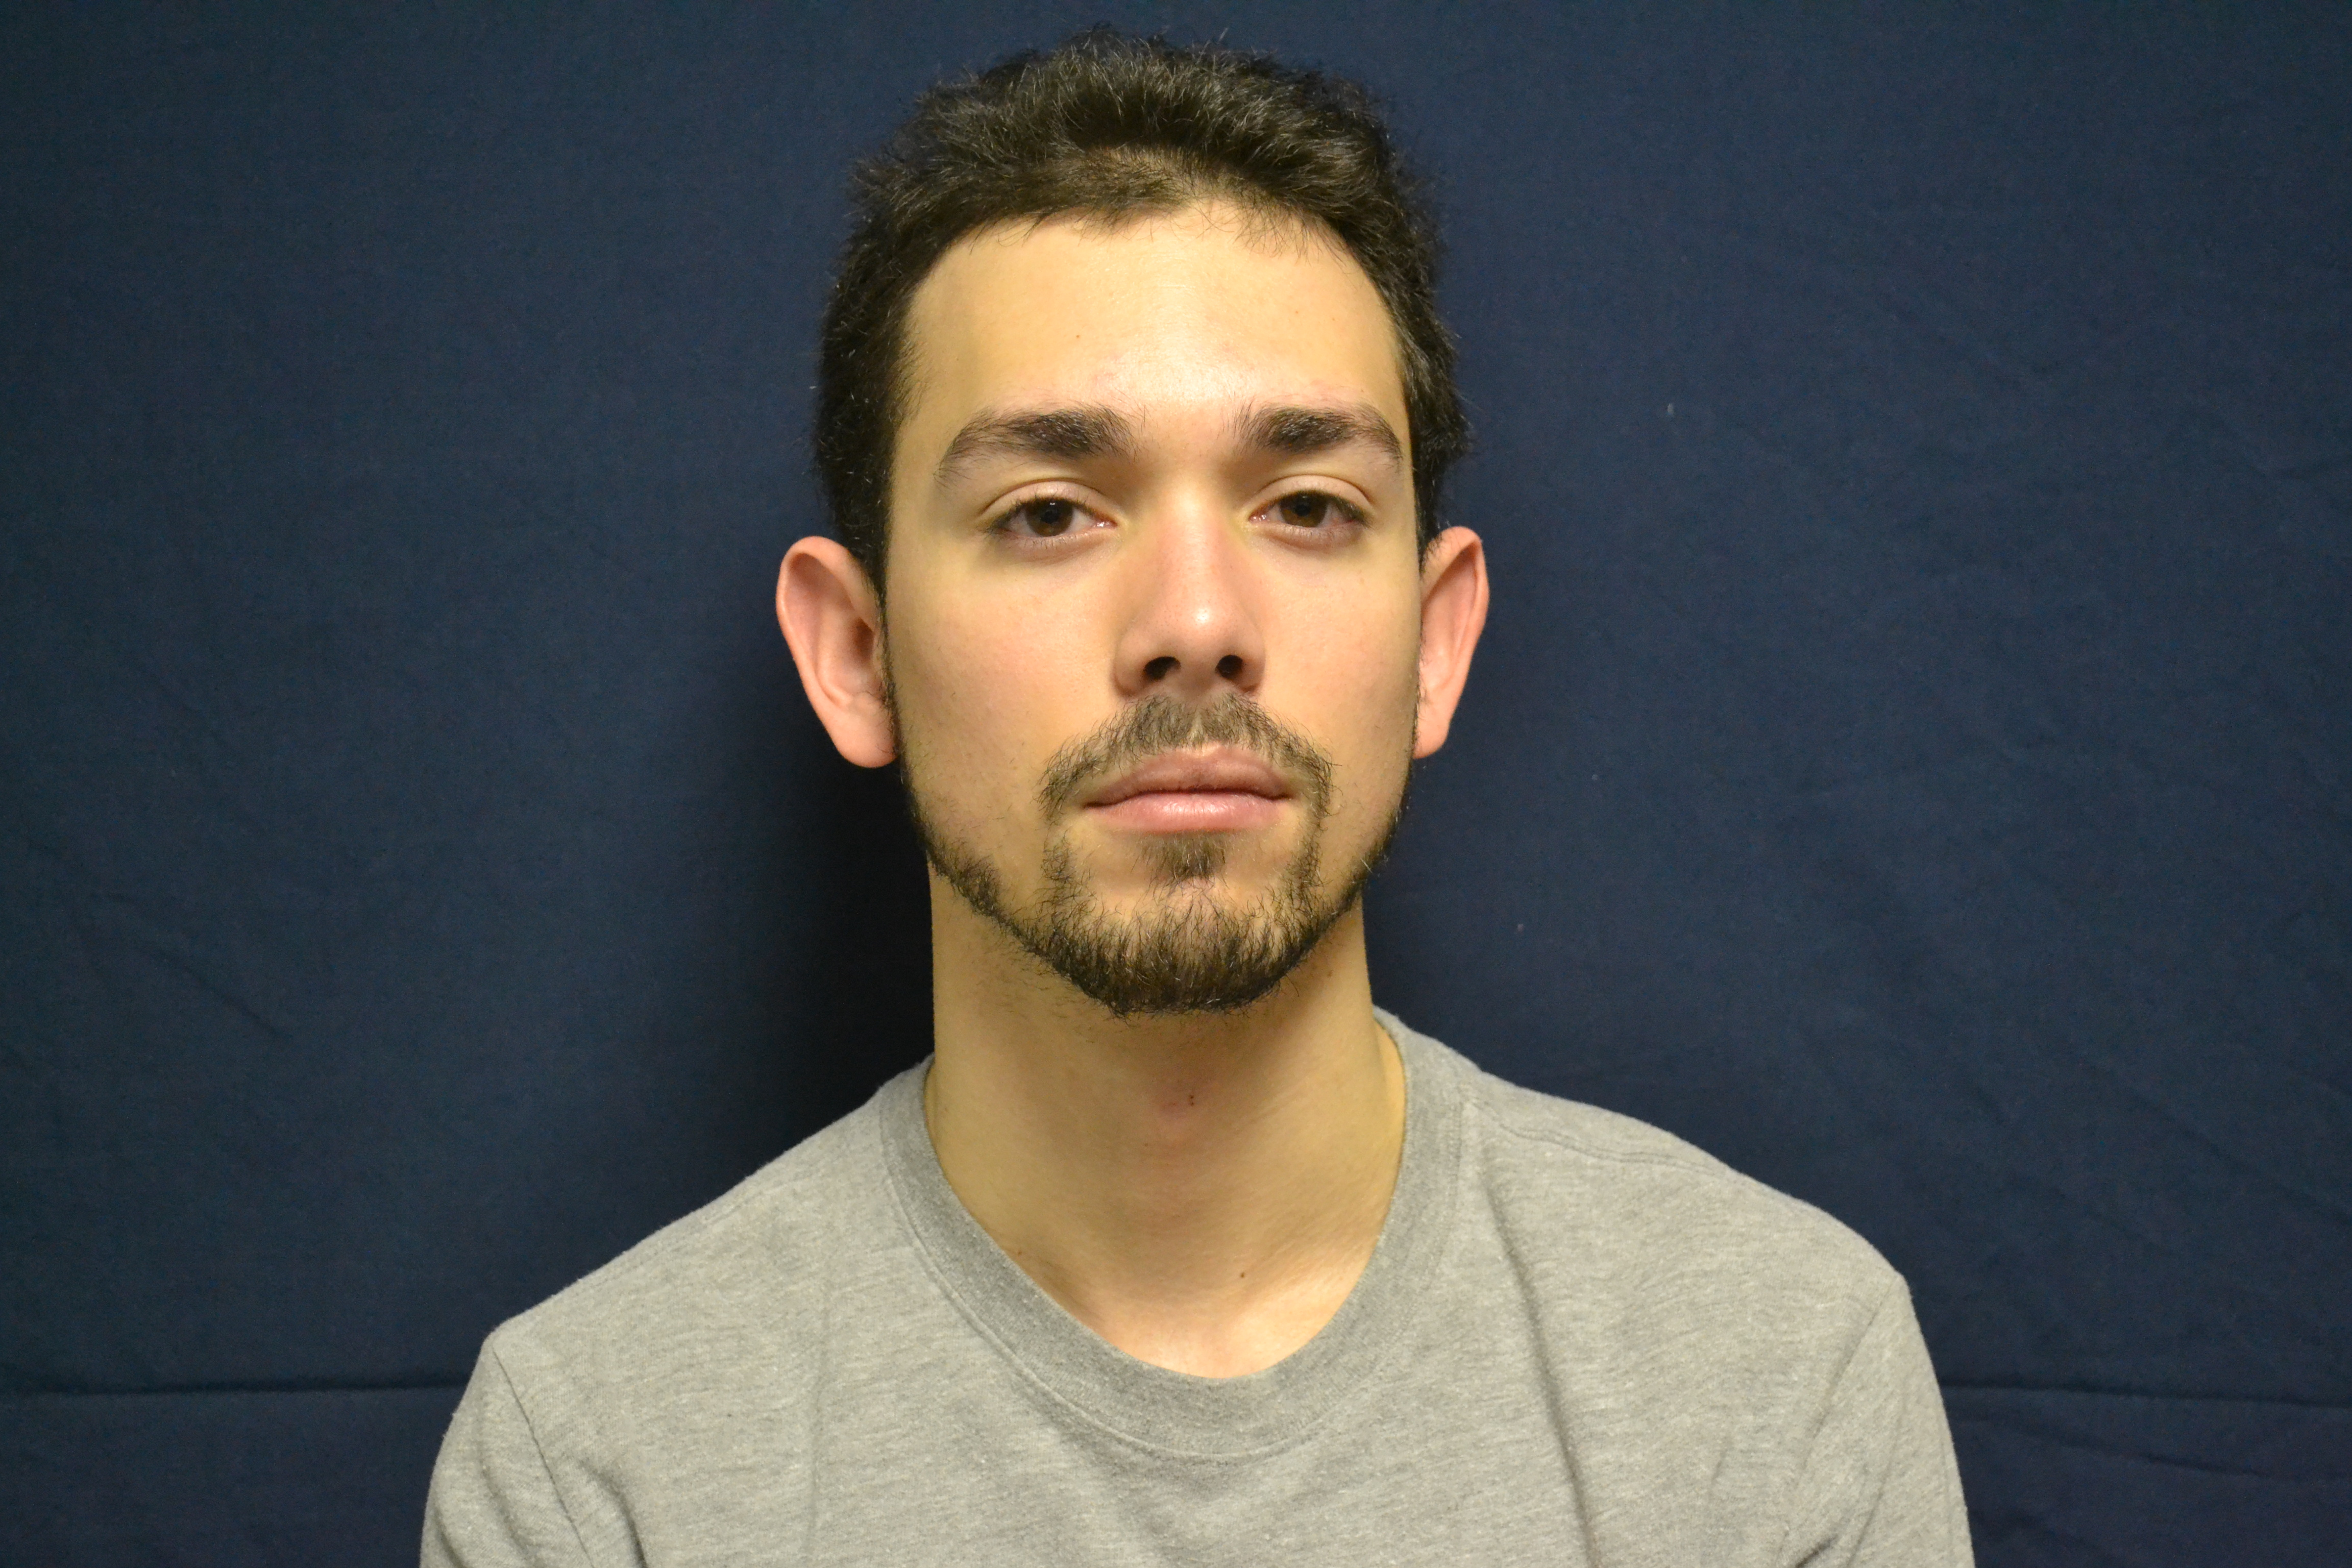
\includegraphics[scale = 0.15]{figures/ExcellentImg.jpg}
        \label{fig:excellentImg}\hspace{1.5cm}}
    \subfloat[Facial image with defects]
        {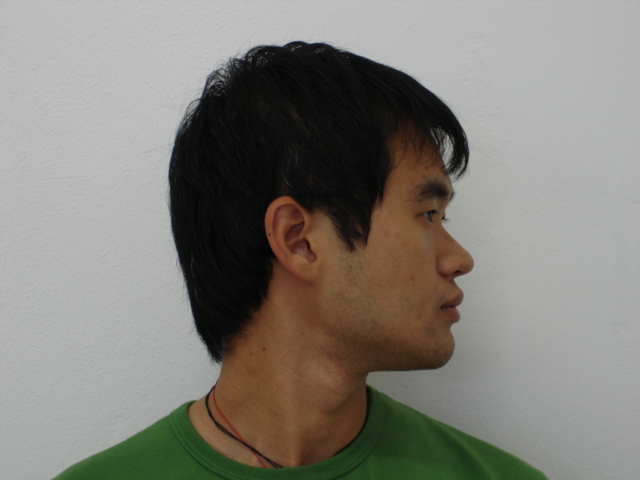
\includegraphics[scale = 0.23]{figures/FairImg.jpg}
        \label{fig:defectedImg}}
    \caption{Difference in face quality}
\end{figure}

Image \ref{fig:excellentImg} checks all bullet points in what defines an excellent image. The subjects' facial expression and head pose is neutral and the whole face is clearly visible. The second image \ref{fig:defectedImg} however does have some flaws. The main reason these two images greatly differ in quality is because of the head rotation. The head is rotated 90 degrees to the side which makes vital parts of the face far less visible. The facial image with defects does have a neutral background with good lightning and image resolution, but those aspects does not weight up against the head pose.
\newpage

\begin{figure}[h]
\centering
    \subfloat[Use of face coverings]
        {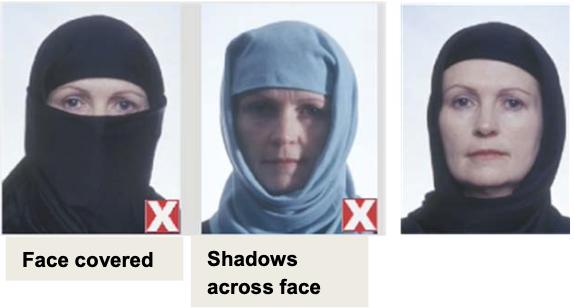
\includegraphics[scale = 0.55]{figures/FaceCovered.png}
        \label{fig:faceCovered}}
    \subfloat[Use of glasses]
        {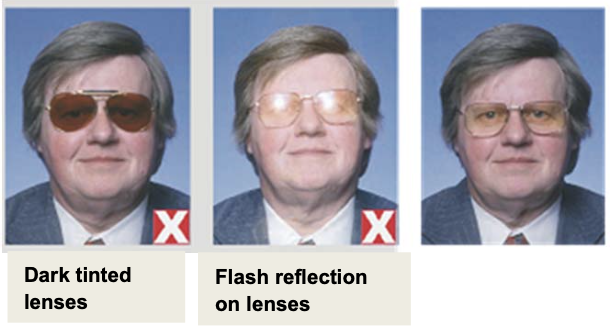
\includegraphics[scale = 0.55]{figures/SunglassesTinted.png}\hspace{1.3cm}
        \label{fig:glasses}}
        \vspace{0.5cm}
        \newline
    \subfloat[Facial expressions]
        {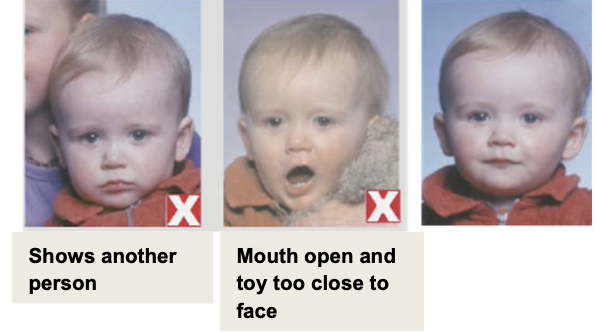
\includegraphics[scale = 0.55]{figures/BabyOpenMouth.png}
        \label{fig:babyMouth}}
    \caption{Subject lineups \cite{ICAO1}}
    \label{fig:ICAOlineup}
\end{figure}

The three image lineups in Figure \ref{fig:ICAOlineup} showcases typical flaws of facial images that negatively affect the quality. The last image of each lineup is considered to have the best quality. The flaws described varies in severity. The face image quality of the lady with her face covered would be at the bottom of the quality scale. The first two images of the man, would not affect the quality to the same degree and the quality of the first two images of the kid, would affect the quality even less. 
\newpage

\section{Face image quality metrics} 
With the inclusion of authentication to applications, face recognition (FR) systems are being utilized more than ever. These FR systems are reliant on a reference image, which is pre-captured, to compare with a probe image for identity recognition. 

\begin{figure}[h]
    \centering
    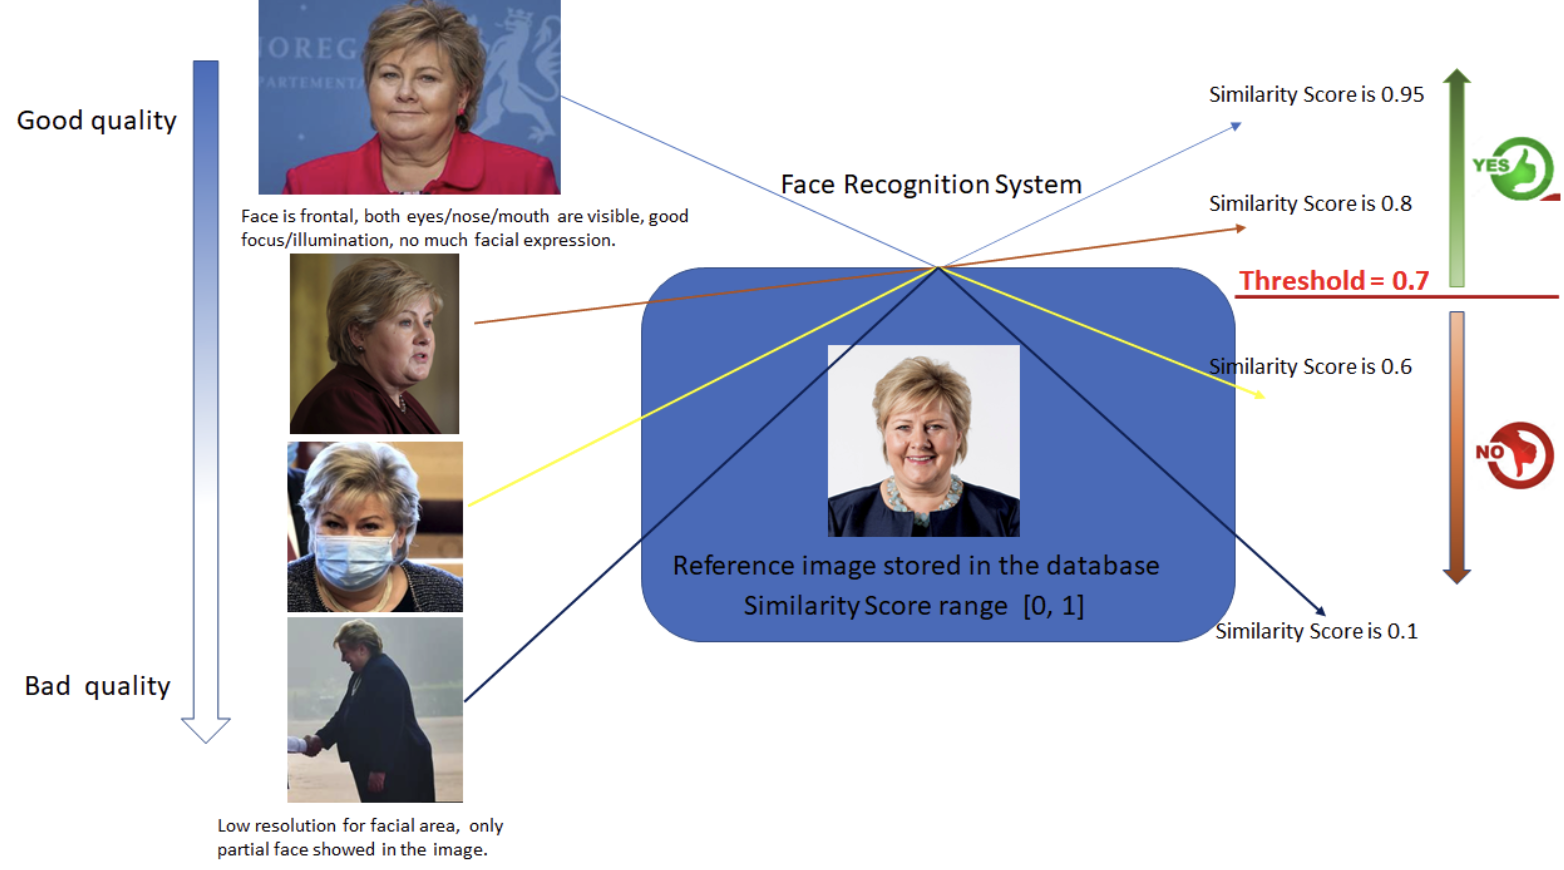
\includegraphics[scale = 0.45]{figures/Erna.png}
    \caption{Face recognition system}
    \label{fig:erna}
\end{figure}

Figure \ref{fig:erna} visualizes how FR systems work. The probe images´s qualities, on the left side of the figure, are assessed and then used to compare with a reference image. The reference image is of the best quality. A similarity score between the two images is calculated, and in this case the similarity score is between zero and one. FR systems have a set threshold where probe images are rejected if the similarity score is too low. 

As mentioned in Section \ref{section:background}, Mobai is currently using such a FR system. The performance of the system is affected by the quality of the probe images. If the probe images are of bad quality, the overall performance of the system will be degraded. This is where the FIQMs are relevant. The metrics can be used to reject and filter images of low quality and therefore only allow images of high quality to be used in the FR system. 
\newpage

\begin{figure}[h]
    \centering
    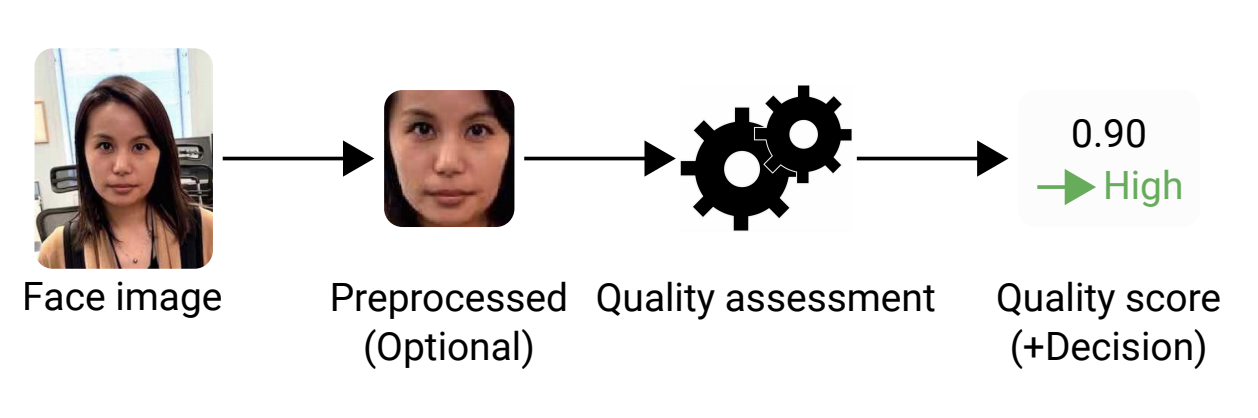
\includegraphics[scale = 0.45]{figures/FIQM.png}
    \caption{Typical FIQM process \cite{FaceImageQualityAssessment}}
    \label{fig:fiqm}
\end{figure}

FIQMs are automated algorithms that take images as input, does some calculations, and return a quality estimate score. FIQMs can be based on different quality factors, such as subject-camera distance, inter-eye distance, pose, lightning and facial coverings. 

FIQMs can be divided into three approaches in regards to a reference image. It is important to understand that these reference images have nothing to do with the reference images mentioned in the FR system. These reference images are only used for the FIQMs. The three approaches are: 

\begin{itemize}
    \item Full-reference.
    \item Reduced-reference.
    \item No-reference. 
\end{itemize}

The names of the approaches are telling of what to expect. The full-reference approach compares the input image against a known reference image of good quality. The reduced-reference approach is similar to the above mentioned approach, however only some of the information in the reference image is used. At last, the no-reference approach does not require a reference image to calculate a score. 

Mobai chose the FIQMs used in our application. The reason for choosing these specific metrics was their differences in terms of evaluating images of faces. The two FIQMs are both no-reference approaches which will be used to assist and provide feedback when an image is acquired for FR system enrollment. 


\subsection{ISO metrics}
ISO metrics is a non-referenced face image quality metric. The metric is implemented based on ISO/IEC TR 29794-5:2010 Information technology — Biometric sample quality — Part 5: Face image data. Different factors that affects the face image quality are considered in the implementation. 

\subsubsection*{Filter by eye distance}
The ISO metrics calculates the inter-eye distance on facial images passed in the metric. If this value is below a certain criteria, the metric will filter out these type of images. The inter-eye distance is related to subject camera distance, because it indicates that the subject could be too close to or too far from the camera lens. 

\subsubsection*{Image properties and characteristics}
\label{subsubsection:image properties and characteristics}
ISO metrics takes all image properties and characteristics described in the ISO paper into account when evaluating facial images. It calculates the image's sharpness, contrast, blur, brightness, exposure, pose symmetry, light symmetry and illumination symmetry. These factors are stored in an array for each facial image. 

\subsubsection*{Predicting the quality score}
To be able to calculate quality scores on the facial images, train data are needed. The metric uses random forest regression \cite{RandomForestRegressor} with 214 trees, 22 nodes of depth and the dataset is used to build each tree. Quality scores of the facial images are computed by predicting the image properties array described in \ref{subsubsection:image properties and characteristics}. 

\subsection{FaceQnet}
FaceQnet \cite{FaceQnet} is an open source, no-reference face quality assessment tool based on deep learning. FaceQnet has two versions implemented, FaceQnet v0 and FaceQnet v1. The newest, FaceQnet v1, was used for this project. Its quality measures is closely related to the ICAO \cite{ICAO2} standard that provides strict guidelines for capturing images. Factors such as illumination, pose, resolution and focus are essential in regards to the quality.

\subsubsection*{Face cropping}
In figure \ref{fig:fiqm} the second step, data preprocessing, is optional. That step is key in the implementation of FaceQnet. Generally data preprocessing removes unnecessary data, which directly improves the quality of machine learning algorithms. 

The background of images will affect the quality score which provides us with biased results. One way to avoid feature extraction from the background, is to crop the input images to only match the face before using FIQMs. FaceQnet uses multitask cascaded convolutional networks (MTCNN) to detect and extract the coordinates of the faces. Thereafter the facial image is cropped to an $224 \times 224 \times 3$ image according to the bounding box and used as the input image to the FIQM. 
\newpage

\subsubsection*{Training data}
FaceQnet uses the VGGFace2 \cite{VGGFace2} database to create a pretrained model to make its quality prediction. The VGGFace2 database is quite large with over 3.31 million images of 9131 subjects which is why FaceQnet only uses a subset of 300 subjects. The algorithm will first generate ground truth quality measures which is created by labeling the 300 subjects in the training database. The ground truth quality measures will then train the deep regression model in order to generate quality scores. After the model is trained, it is ready to receive the probe images. The data provided to the FIQM is loaded and split into test data (X\_test and y\_test) which are used to get a quality estimate. 


\chapter{Objective Assessment}
\label{chap:objective}
This chapter contains the development process of the Face Quality Analysis application. To start we will look at functional and non-functional requirements in Section \ref{sec:requirements} followed by use cases in Section \ref{sec:useCase}. Section \ref{sec:choiceOfFrontBack} discusses our choice of front- and backend implementation, followed by Section \ref{sec:designAndImplamentation} that shows off our design and implementation. We include sequence diagrams in Section \ref{sec:sequenceDiagram} to show how some of the core functionality work.

\section{Requirements}
\label{sec:requirements}
When approaching the requirements, we had to make decisions based on the task description as well as the meetings with Mobai. The description and Mobai were open in terms of setting requirements, but some core concepts of the desired product were simplicity, clarity, performance and modifiability. Based on these principles, we along with Mobai shaped non-functional and functional requirements. Also, as mentioned in Section \ref{sec:OurModel} not all requirements were set at the start of the project, so they had to be fine-tuned and confirmed during the development process. While this did not result in any dramatic change in the software, as more functionality were suggested, requirements had to be adjusted to address to these issues. The non-functional requirements describes how the software should perform. These are the following requirements:
\begin{itemize}
    \item The application should be deployed in a container.
    \item The architecture should consist of a backend and a frontend.
    \item APIs should be implemented as REST APIs.
    \item The application should make it easy to add new FIQMs.
\end{itemize}
The functional requirements defines what the software should do or not do. These are the following requirements:
\begin{itemize}
    \item The application should run every available FIQM separately.
    \item The application should run all FIQMs together.
    \item The application should return a report with quality scores on every image based on the FIQMs as a \acrshort{json} file.
    \item If only one image is evaluated, the image should be displayed with corresponding attribute scores. 
\end{itemize}

\subsection{Type of Application}
The responsibility of choosing application type was given to the bachelor group. Selecting either a web or desktop application was challenging, but we carefully evaluated the type of application that suited our needs the best. 

\subsubsection*{Desktop Application}
Since desktop applications are downloaded to your operating system, they are available independently whether you are connected to the internet or not. In that way it is possible to stay functional all the time \cite{WebVsDesktop}. The constant accessibility that desktop applications provide automatically make them more secure. In a way, you never have to be connected to the internet when working on tasks which reduces the possibility of being hacked by a margin. Having a fast computer would be beneficial for running a desktop application. The application uses memory and CPU which returns a good user experience given a resourceful computer. However, using an old computer would not be a problem either. The fact that desktop applications allows for running older versions of the program with all functional availability does not make a hardware upgrade necessary. Also, given that desktop applications do not coerce to update, the software makes it adaptable to choose a suitable version for the computer's specifications. It is also uncomplicated to store files from the application, as information are supported by the computer's hard drives. 

Naturally, desktop applications have their downsides as well. The application may require multiple updates to enable full functionality which seems persistent and unnecessary. If the work is performed on different devices, each device need the same installation to synchronize the progress. This will also make it more challenging for multiple users to collaborate on desktop applications. Another disadvantage with a desktop application is its dependence on operating system requirements. To allow the latest functionality the application provides, specific requirements are required. 

\subsection*{Web Application}
A web application only require one installation step before the software is workable \cite{WebVsDesktop}. This is time saving because it provides the user access to the web application by typing the internet address into a web browser on any operating system. All updates are free and immediately available. The ease of availability for these applications make synchronizing with several devices a small matter. In addition to this, the simplicity of managing cooperation with different users is remarkable. While some licence issues may arise, but this solution still allows the users the chance to collaborate from their permanent working stations.

When it comes to the disadvantages of web applications, they require a constant internet connection. In addition, the application's capability depends on the internet connection and speed. A poor connection and speed could result in a bad workflow. As regular updates could be beneficial, there are less possibilities of using older versions of the software. 

\subsection*{Our Application}
Keeping in mind the mentioned advantages and disadvantages, in our work, we chose to build a web application. Given the intuitive user interface with a limited amount of functions, it was practical and more meaningful to develop a web application. We felt a desktop application would be more suitable if the application requirements increased and the programming tasks were more complex. Our web application would be time saving and comprehensible for Mobai employers since the application only need one installation before working on the software. When new FIQMs are added to the application, the update is easily done and users can instantly evaluate facial images with the new incoming metrics. 

\section{Use Case}
\label{sec:useCase}
We have created a use case diagram  showcased in Figure \ref{fig:UseCase} along with use cases in Table \ref{usecase:uploadImages}, \ref{usecase:runFIQM}, \ref{usecase:deleteImages} and \ref{usecase:runAllFIQM} to show the core functionality and activities within the application. The diagram was built from the perspective of the user (described in Section \ref{sec:TargetGroups}) which were employees at Mobai. The cases differ in complexity where running all metrics would be the most challenging. That is because it includes running every metric and providing scores for each image. 

\begin{figure}[h]
    \centering
    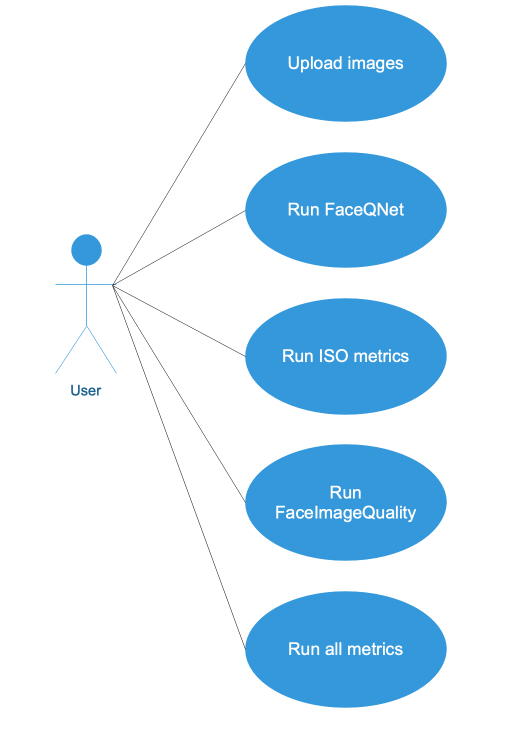
\includegraphics[scale = 0.4]{figures/UseCaseDiagram.png}
    \caption{Use case diagram.}
    \label{fig:UseCase}
\end{figure}

\newpage

\begin{table}[h]
\caption{Use case: Upload images.}
\label{usecase:uploadImages}
\centering
\resizebox{\textwidth}{!}{%
\begin{tabular}{|p{12cm}|} 
\hline
\textbf{Use case:} Upload images\\
\textbf{Actor:} User \\
\textbf{Goal:} Upload selected images \\
\textbf{Description:} The user can select what images he would like to upload to the application. Images will only be stored in the application in that session. \\ \hline
\end{tabular}%
}
\end{table}

\begin{table}[h]
\caption{Use case: Run FIQM.}
\label{usecase:runFIQM}
\centering
\resizebox{\textwidth}{!}{%
\begin{tabular}{|p{12cm}|} 
\hline
\textbf{Use case:} Run FIQM\\
\textbf{Actor:} User \\
\textbf{Goal:} Evaluate images with a specific FIQM \\
\textbf{Description:} After uploading selected images, the user would run a specific FIQM to assess the images. The application returns a report with quality scores for each facial image. \\ \hline
\end{tabular}%
}
\end{table}

\begin{table}[H]
\caption{Use case: Delete images.}
\label{usecase:deleteImages}
\centering
\resizebox{\textwidth}{!}{%
\begin{tabular}{|p{12cm}|} 
\hline
\textbf{Use case:} Delete images\\
\textbf{Actor:} User \\
\textbf{Goal:} Remove images from the session \\
\textbf{Description:} After running the FIQMs for the uploaded images, the user is able to remove all images used in that session. \\ \hline
\end{tabular}%
}
\end{table}

\newpage

\begin{table}[h]
\caption{High level use case for ``Run all FIQMs''.}
\label{usecase:runAllFIQM}
\centering
\resizebox{\textwidth}{!}{%
\begin{tabular}{|l|p{9cm}|} 
\hline
\textbf{Case} & Run all metrics  \\ \hline
\textbf{Description} & The user runs all metrics in the application which returns scores for every image.      \\ \hline
\textbf{Basic Flow} &   \begin{enumerate}
    \item The user presses the ``upload images'' button.
    \item The user navigates to select wanted images to execute the metrics on.
    \item After uploading images, the user presses ``Run all metrics''
    \item The program returns a report with quality scores of the selected images
\end{enumerate}     \\ \hline
\textbf{Alternative} &  The user runs all metrics without uploading any images
            \begin{enumerate}
                \item The application displays an error and asks the user to upload images.
            \end{enumerate}
The user presses reset before running the metrics 
            \begin{enumerate}
                \item Uploading images again is necessary.
            \end{enumerate}
                    \\  \hline
\textbf{Pre-condition} & The application is running and images are uploaded. \\ \hline
\textbf{Post-condition} &  The FIQMs have predicted the perceived face quality on the images. \\ \hline
\end{tabular}%
}
\end{table}

%\clearpage


\section{Choice of Front- and Backend}
\label{sec:choiceOfFrontBack}
When choosing the development software, we had to take some considerations. First, both backend and frontend software should not be time consuming to master, given that the project consisted of coding and research. Second, it should be uncomplicated to add the released FIQMs with the backend as well as creating an intelligible user interface. 

\subsection{Backend}
The two FIQMs FaceQnet and ISO Metrics were written in Python. Since we were experienced with Python and operated with it in courses throughout the bachelor program, it was natural to choose a Python framework for the backend. With a dozen of possible web frameworks, we needed to select a framework which suited our needs in terms of scalability, performance and ease of use. In the end, the choices were between Django and Flask.

\subsubsection*{Django}
Django is a fast framework, which quickens the development process for developers. It has a high level of scaliability to the users. This feature is the reason many leading websites depend on Django to fulfill their high operational requirements. The framework includes several rebuilt development features such as user authentication, sitemaps and content administration. It has excellent security, preventing the users from several security issues. Django is very flexible as it can be used to create a wide specter of application types. Some of these are social networking sites like Instagram or content management systems such as Wagtail \cite{DjangoAdvantages}.

When it comes to the disadvantages, Django has a steep learning curve. Even though it its written in Python, it takes a long time for developers to get the hang of it. The framework is considered one of the hardest to master. Django is more suitable for large scale applications rather than smaller products with fewer features and requirements. The unique functionalities within Django can be confusing for developers working with a small project. Djangos' monolithic architecture has a small number of dependencies which make it challenging to use. It does not facilitate developers to utilize Python packages and tools, but focuses on code-oriented programming. Django can not provide fast development in terms of requests. Only one request at the time can be fulfilled, meaning it is unable to handle multiple requests concurrently \cite{DjangoDisadvantages}.

\subsubsection*{Flask}
\label{sec:flask}
For programmers with experience in Python, it is easy adaptable to work with Flask. This micro framework is simple to manage as there are few standards. Flasks' modular nature let developers instantly create servers and applications, which are distributed across comprehensive networks with certain purposes. It is pliable, meaning that components within the framework are easy to modify, because it is simple to configure. Given that Flask is a micro framework, it has less abstraction layers between the users and the database, cache and requests. This design provide users high level of performance \cite{DjangoAdvantages}.

Flask also has some disadvantages. Many beginner web developers tend to use the Flask framework, resulting in low quality code and possibly a bad application. Flask has singular source, meaning that it handles requests in turns. With multiple requests, it could be time consuming to handle the requests. The use of modules in Flask raises security issues. It would be bad if a module contained spiteful data. 

\subsubsection*{Our Choice}
Initially, we started the backend development process using Django. This was mainly because the team working with the backend had learned about the framework in an earlier course of the bachelor program. However, we eventually concluded not to use Django for the backend. Given some knowledge in the framework, we had not actually developed anything with it. Since Django did not provide the usage of Python packages or tools, it would be more time consuming to code the application. The steep learning curve provided by the framework would make the development process even more time consuming. Our project differed in working tasks, which made the application smaller in terms of features and requirements. Django was more suitable for larger applications, making the decision of not using the framework clearer. We ended up using Flask for the backend. Immediately after installing the framework, the development productivity increased. Our Python experience was easily adaptable to Flask, which made it simple to make a deployable application and add FIQMs in the program. 

\subsection{Frontend}
As mentioned in Section \ref{sec:requirements}, the central ideas of how Mobai wanted the application to be built were simplicity, which was adaptable when choosing how to build the frontend. Mobai's vision was for it to be a demo to show some of the key concepts provided by the backend, like displaying results from different FIQMs on a small amount of images. It could also be used as a demonstration to Mobai's customers. Since we decided to build the frontend as a web application, we quickly understood that this would be coded in HTML, CSS and JavaScript. 

The backend framework Flask explained in Section \ref{sec:flask} has a way of rendering simple HTML pages by itself. In the early stages of our development, we built a simple HTML page consisting of buttons and text and had Flask render the template. This was a good way of testing the backend functionality. Using this method would simplify the frontend and make the application run solely on the backend port 5000. The problem with this method was that the HTML pages rendered were quite static and had restrictions in form of design and functionality. This also meant that the frontend would be incorporated into the backend, and the backend had to be started in order for the frontend to work. After a discussion with Mobai, we found out that this was not the best solution. 

We wanted the frontend to run independently from the backend on its own server. This way, the frontend would not be dependent on the backend to run, and we would get more flexibility when it came to design and implementations. We could still program the frontend using basic HTML and JavaScript, but we found that using a well-developed web framework would enhance the design and simplify for future development of the application. Angular and React are the two frameworks we considered to use. 

\subsubsection*{React}
React is a JavaScript library, but is often referred to as a whole framework because it is directly comparable to other web development frameworks. React is component based, which means the user interface can be rendered using different components. By doing this, the same component can be rendered multiple times without duplicating code and it will be easier to fix bugs because they are likely caused by one specific component. This is one of the key factors that makes React flexible and dynamic. This also makes React applications easier to test and maintain. Considering it is a JavaScript library, learning is easier for any developer that has a JavaScript background, and also more lightweight than other frameworks. React uses its own virtual \acrfull{dom}. This DOM is a cross-platform and programming API which deals with \acrshort{html}, \acrshort{xml} or \acrshort{xhtml}. The React virtual DOM exists entirely in memory and is a representation of the web browser's DOM. This means that when we want to render React, the virtual components will turn into the DOM, leading to smoother and faster performance \cite{ReactProsAndCons}.

React has a high pace of development, which can be both an advantage and a disadvantage. Since the environment constantly changes, some developers might not feel comfortable relearning the new ways of doing things regularly. It may be hard to adapt to new ways of doing things constantly and always be updated. Because of the constant updating, the technology is accelerating so fast that there might not be enough time to make proper documentation.

\subsubsection{Angular}
Angular is an open-source software engineering platform used to build UIs. The main benefit of using Angular is to turn static HTML-based documents into dynamic content using components. It was built on the \acrlong{mvc} architecture, where the framework is synchronized with the model and the view. This is called two-way binding. This allows developers that use Angular to reduce the development time as it will not require additional code to synchronize the model and the view. Angular uses something called dependency injection. Dependencies define how different pieces of code interacts with each other and how changing one component affects others. Using dependency injection, dependencies can be defined externally outside components, making the dependencies decoupled from the components. This makes components more reusable, easier to manage and test \cite{goodBadAngular}.

When it comes to the disadvantages, Angular is a framework that always has multiple ways of completing any task. Therefore the framework has a steep learning curve. Due to Angular's two-way binding, it may sometimes cause performance issues when rendering multiple components, especially on old devices \cite{AngularCons}. Since Angular is a complete framework, it is created for building enterprise-scale applications, making the framework less flexible than other lightweight frameworks \cite{goodBadAngular}.

\subsubsection{Our Choice}
We ended up choosing React, considering its great performance, flexibility and its ability to create dynamic web pages. React has its own Command Line Interface (CLI) tool that makes building a React app easy. This command is called ``create-react-app'' and automatically builds up all files, packages and folders that are needed to run a React application \cite{ReactGetStarted}. The command also serves the React app with a server using Node.js, which is an open source, cross platform, JavaScript runtime environment that gives the ability to run web pages on server side \cite{NodeJs}. In order to run the CLI tool, Node.js would have to be installed first. Using this method, a React application could easily be installed and the web page be run on a local server on port 3000 using the Node.js command ``npm start''. This way we have created a frontend independent of the backend running on port 3000.  

\section{Design and Implementation}
\label{sec:designAndImplamentation}
In this section we will explain the design of our front- and backend applications, as well as show some key implementations from the requirements and use cases.  

\subsection{Backend}
The backend's implementation and functionality were developed using purely Python. The Flask framework explained in Section \ref{sec:choiceOfFrontBack} is used to communicate with the frontend. When we start the backend, the Flask framework will start a server running on port 5000 on the local computer. From there, Flask will wait for HTTP requests in forms of GET or POST and execute the code based on what request was sent. This is what we call the REST API. Code listing \ref{lst:APICall} shows how we have implemented a REST API call for the use case ``Run all metrics'' showcased in the use case diagram in Figure \ref{fig:UseCase}. 

 \lstinputlisting[
     caption={API call implementation.},
     label=lst:APICall,
     language=Python,
     numbers=left,
     xleftmargin=2.5em %5.0ex %For å justere linjenumrene 
 ]{listings/all-algorithms.py}

This code is run when the backend receives an API call with a route to ``/allAlgorithms''. The code checks if there are images uploaded to the backend, and if there are, all FIQMs are executed on the uploaded images and the results will be written to one single file for all metrics and sent to the frontend for display. This function returns a JSON file that gets sent to the frontend. This is because of a request Mobai had to save the results in a JSON format in case the data were going to be modified or used in the future. Our implementations for all use cases in our application follow the same structure as in Code listing \ref{lst:APICall}, but with different routes and code. 

For Mobai, the possibility to easily add more FIQMs into the backend was important, and one of the reasons why we chose to have an API call that can run all the metrics in one go. To simplify the process of adding more FIQMs, we have created independent functions in Python that do not rely on any FIQMs to work and can be used for multiple purposes in the future. Two of these functions are called ``save\_results\_to\_file'' and ``save\_results\_to\_json'' and are used in Code listing \ref{lst:APICall} to combine the results from both FIQMs into one single file, either in JSON or CSV format. Another step we took to simplify the adding of new FIQMs was to restructure the metrics code into Python functions. This way, we could run the different FIQMs by calling its specific function, and then save the results using the function ``save\_results\_to\_file''. These are options that make it easier for Mobai to add new metrics to the backed and reuse the code that we have already created. 

Mobai also wanted the backend to work independently on the frontend, meaning that all functionality available in the frontend should be able to run in the backend alone. This includes running FIQMs and uploading images. Uploading images can be done by simply drag-and-dropping images into the ``Uploads'' folder in the backend, but running the FIQMs would require accessing the REST API without the use of the frontend. To solve this, we used another third party software to send HTTP requests to the backend. Postman is such an application that can simulate a client and send POST and GET requests to the backend. By using Postman, we can send a POST request to the backend and get the returned results from a JSON file displayed. Figure \ref{fig:postman} shows a POST request being sent to the backend using postman and then displaying the results from the JSON file. Consider the code in Code listing \ref{lst:APICall} to run when the API call gets sent. 

\begin{figure}[h]
    \centering
    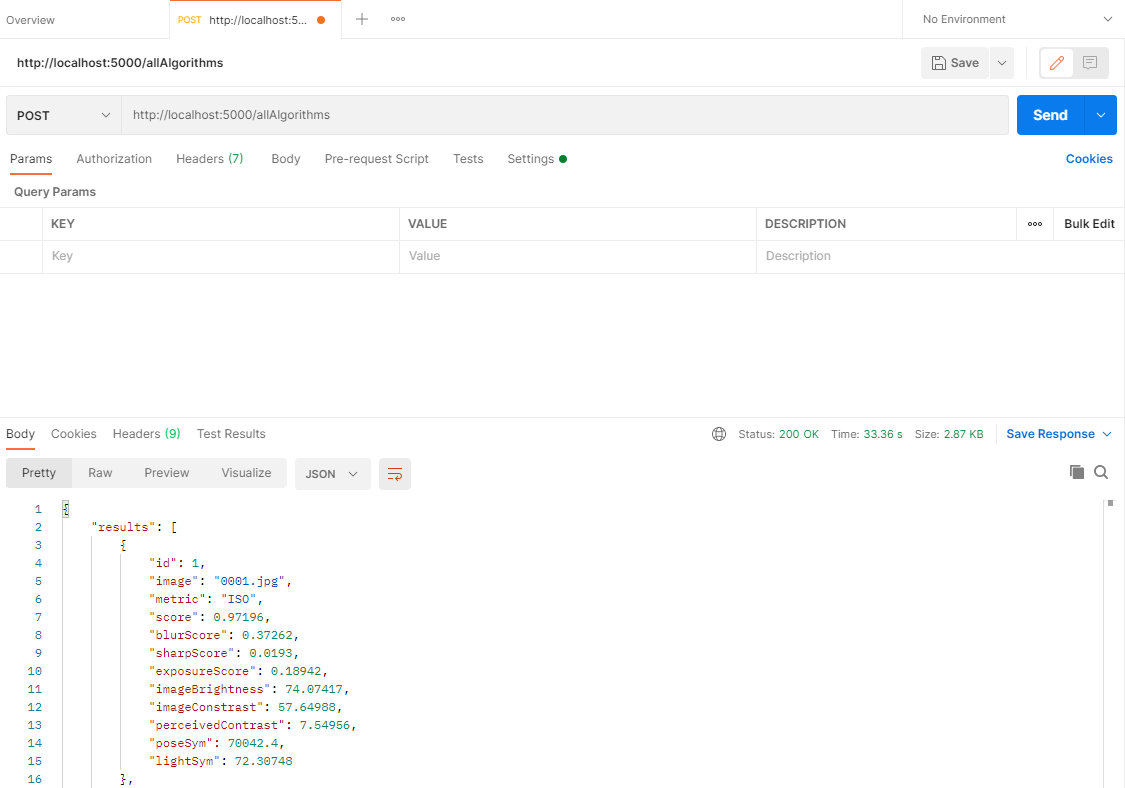
\includegraphics[width=0.9\textwidth]
    {figures/postman_json.PNG}
    \caption{POST request with Postman.}
    \label{fig:postman}
\end{figure}
%api calls implementation, adding more metrics, different routes, write to file, send file to frontend. use 3rd party software to communicate with the backend 

\subsection{Frontend}
Due to Reacts popularity, multiple UI frameworks has been built to simplify the process of building web pages. One of these frameworks are called Material-UI. Material-UI delivers already built components, styles, icons and templates that support the React framework. Most of these components are free and can be used to easily get started with building a web page. When we discussed how to build the web page, we came to a conclusion that using the Material-UI framework would be beneficial to the simplicity, efficiency and design of our frontend. Different Material-UI libraries could be installed using the Node.js command ``npm install''. We also chose to start the development process using a Material-UI pre-built pattern, called ``Album'', that can be found on the Material-UI website \cite{MaterialUI}. 

To build dynamic web pages, React introduced a new addition in version 16.8, called ``React hooks''. This addition provides a way of storing data as a state and the data gets updated automatically once the state is updated. This way we could change text fields, counters and data and display it automatically without refreshing the website, because it is stored in a state. We have used React hooks to store data that we know can be modified during the web applications lifetime. Code listing \ref{lst:hook} is an example of how we have implemented a React hook to store images for the use case ``Upload Images'' showcased in the use case diagram in Figure \ref{fig:UseCase}.

\lstinputlisting[
    caption={React hook implementation.},
    label=lst:hook,
    language=JavaScript,
    numbers=left,
    xleftmargin=2.5em
]{listings/react-hook.js}

The ``imagesSelected'' variable stores the state of what images have been selected from the user, and the ``setImagesSelected'' function updates the state every time a user selects images. If we wanted to display the images selected by the user, setting the variable name in a paragraph would suffice, and React would update the paragraph automatically once the state had been updated.

In order for the frontend functionality to work, the frontend would have to connect to the backend. This is done by sending a \acrshort{http} request in the form of a GET or POST command to the backend. The backend would then execute the specific code in the REST API based on what request was sent. React has different libraries that can send HTTP requests. We have chosen to use Axios to send HTTP request, because it is both compatible with the Node.js framework and can also be installed using the ``npm install'' command. By using Axios, we send HTTP requests from the frontend to the backend. The backend would then return the desired results, either in the form of text or a file. The use case ``Run all metrics'' showcased in the use case diagram in Figure \ref{fig:UseCase} is implemented using Axios.  
Code listing \ref{lst:axios} shows our implementation. 
\newpage
\lstinputlisting[
    caption={Axios HTTP request implementation.},
    label=lst:axios,
    language=JavaScript,
    numbers=left,
    xleftmargin=2.5em
]{listings/axios.js}

Using Axios, we send a POST request defining the port and the route to the backend REST API. The backend then executes all algorithms and returns the results in the form of a JSON file. React saves the results as a state and displays the state dynamically on the webpage. 

%write about material-ui, react hooks,, axios requests

%write about deployment. we dont have to use deployment build, its deployed as a docker container instead, so it can run on port 3000 and 5000 locally. 

\subsection{Deployment}
One of the main requirements given by Mobai was to deploy the application in containers. Containerization \cite{Containerization} provided us with several benefits:
\begin{itemize}
    \item A container is independent of the operating system, making it portable between dissimilar platforms. 
    \item Containers are efficient in terms of allowing applications to quickly be deployed, patched or scaled. 
    \item Containers consume less system overhead than regular hardware or virtual environments owing to the fact that they do not include operating system images. 
    \item Containers provide better application development, production cycles and testing as containers support an agile workflow.
    \item Having the application separated into different containers will improve security. 
\end{itemize}

Once functionality for the application were mostly fulfilled, the task was to package it up into two separate containers - one for the frontend and one for the backend. The basis of containers, images, were created using Dockerfiles. Information that automated the application running process was stored inside the Dockerfiles. This included information such as the base Docker image to run from (i.e., based on Alpine since the application was built in Python), location to project code, dependencies that the application had and which commands to run at start-up. When both Dockerfiles were written, the command ``docker build'' produced two disparate images. To enable both images to run together in a remote environment, we needed to use the Docker Compose tool. We created a Docker Compose file which included the definition of services that built the application. The command ``docker-compose up'' ran the application from our Docker Compose configuration file making the images become containers running on a Docker engine.

\section{Sequence Diagrams}
\label{sec:sequenceDiagram}
In this section, two sequence diagrams, one high level and one low level, will be showcased and discussed. Our web application is simple in design, but behind the scenes several entities are interacting with each other. To firmly understand how the application is constructed, it is essential to acknowledge the interaction between the components. Sequence diagrams are convenient, easy to read tools to visualize a given interaction within a time sequence. Providing both high and low level sequence diagrams will yield a complete picture of our system from a surface to an in-depth level.

%\newpage
\subsection{High Level - ISO Metrics}
Figure \ref{fig:highlevel} is meant as a surface level visualization of what happens the first time the web application is started on a new computer and a metric is executed. After the two Docker images are built, the application is now ready to run. 

\begin{figure}[h]
    \centering
    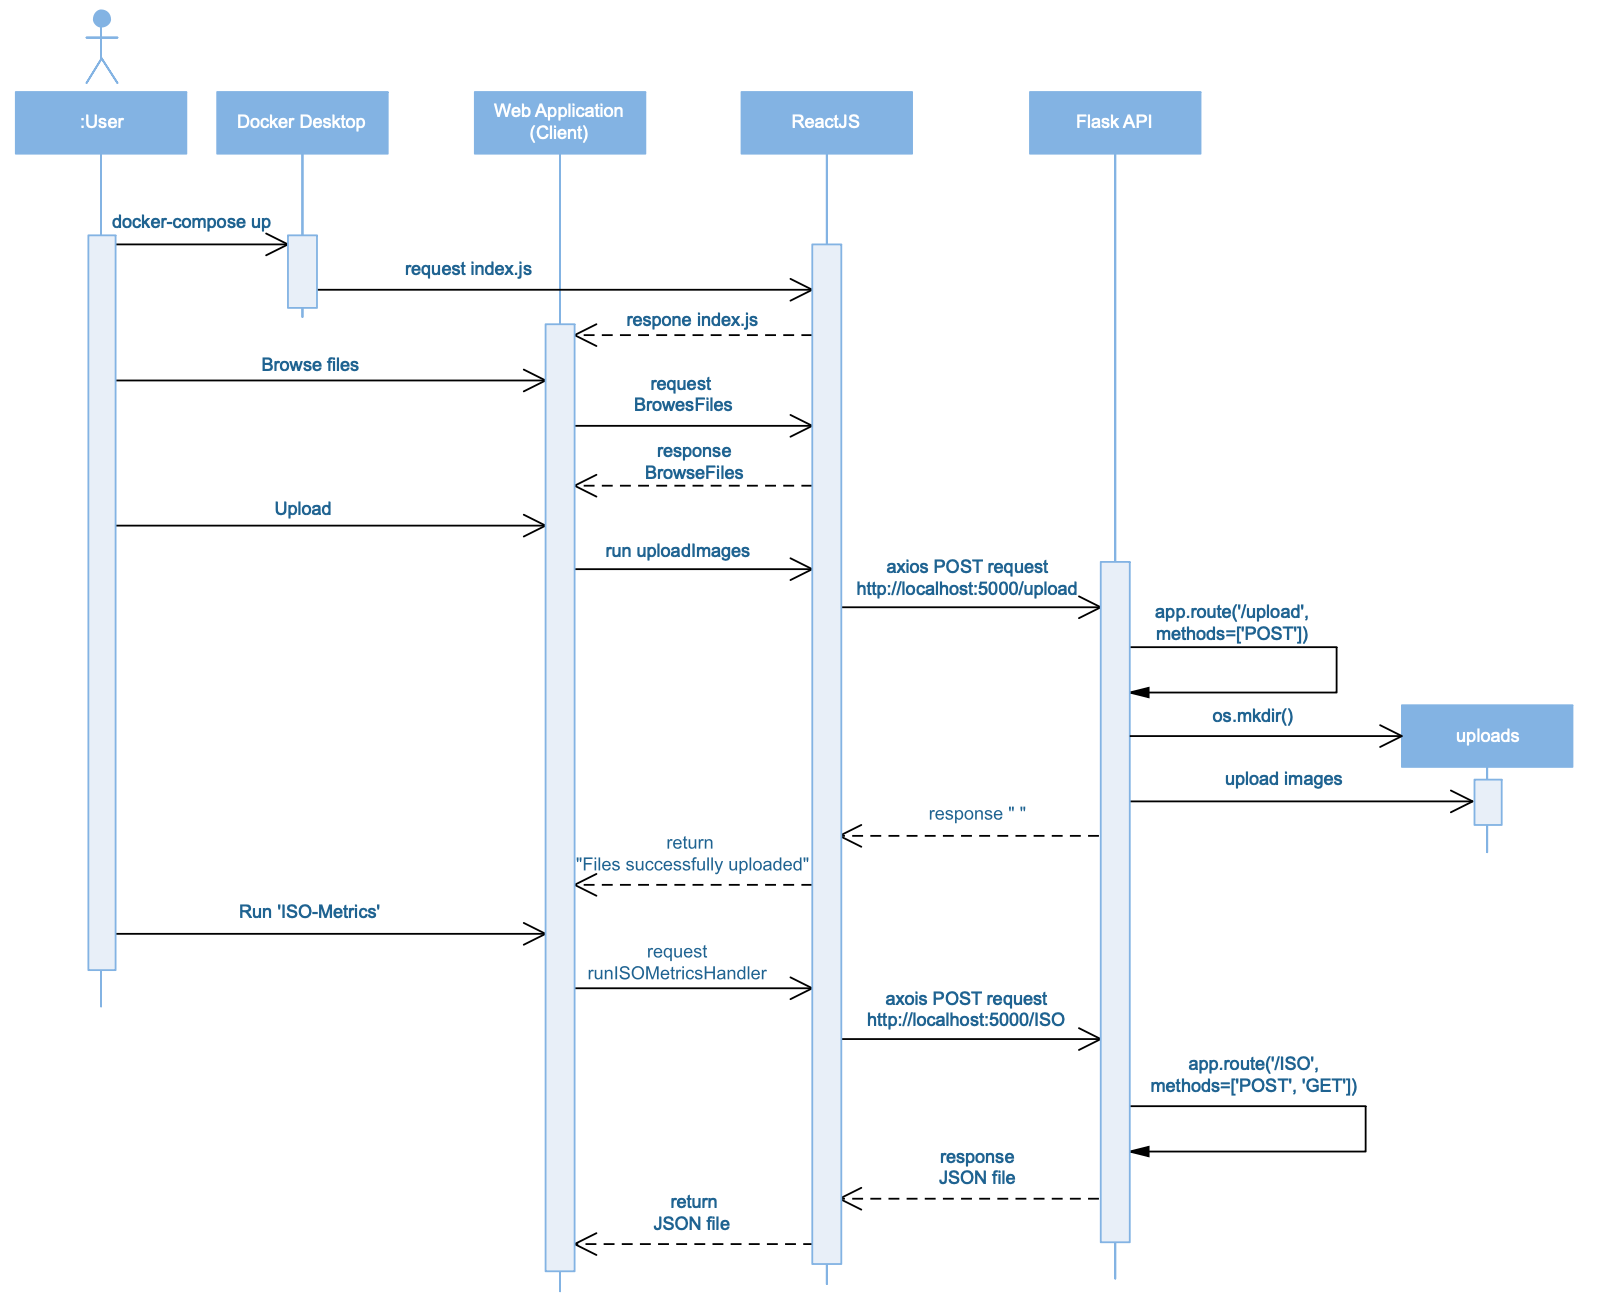
\includegraphics[width=1\textwidth]{figures/HighLevel.png}
    \caption{ISO Metrics: high level sequence diagram.}
    \label{fig:highlevel}
\end{figure}

\raggedbottom

From the terminal window, the command: ``docker-compose up'', will boot up both the React and Flask servers. An immediate request to render the index.js file in the web application is sent to the React server. After the home page is displayed in the web browser, the user can press a button to browse files, which will send a request to the React server to open a window of your local files. Images are now ready to be selected. The selected images are stored in a state that waits for the ``Upload'' button to be pressed. Once the user presses the button, a function called ``uploadImages'' will be executed from the React server that in return redirects an Axios HTTP POST request to the external Flask backend API at port 5000. The POST request contains all the selected images. An API by the name of ``upload'' saves all selected images in a specified ``uploads'' folder in the backend before it is redirected back to the React server that displays a ``Files successfully uploaded'' message to the web application. Since this is the first time the application is executed, the ``uploads'' folder has not yet been created. The upload API therefore has to create it before uploading the images and returning to the web application. 



%\newpage

Once the images are saved in the backend, the web application is now ready to execute any metric. The button ``Run ISO-Metrics'' on the web page is clicked which requests the function runISOMetricsHandler to be executed on the React server. This function will likewise redirect an Axios POST request to port 5000. An API by the name of ISO will receive the request which triggers the API to execute ISO Metrics. Once the metric has generated quality scores on the uploaded images, it returns a single JSON file that contains the scores. This JSON file is returned to the React server which in return displays the scores on the web page. 

\subsection{Low Level - FaceQnet}
Unlike Figure \ref{fig:highlevel}, Figure \ref{fig:lowlevel} is a sequence diagram for how FaceQnet is executed the first time it is ran on a computer. Before the ``Run FaceQnet'' button is clicked, it is given that images have been selected and uploaded to the ``uploads'' folder which is shown in Figure \ref{fig:highlevel}. For that reason, the ``uploads'' folder already exists instead of being created along the way. The first few steps are quite similar to the sequence diagram depicted in Figure \ref{fig:highlevel}, however this time an API called FaceQnet is executed that in return starts the FaceQnet FIQM. 

\begin{figure}[h]
    \centering
    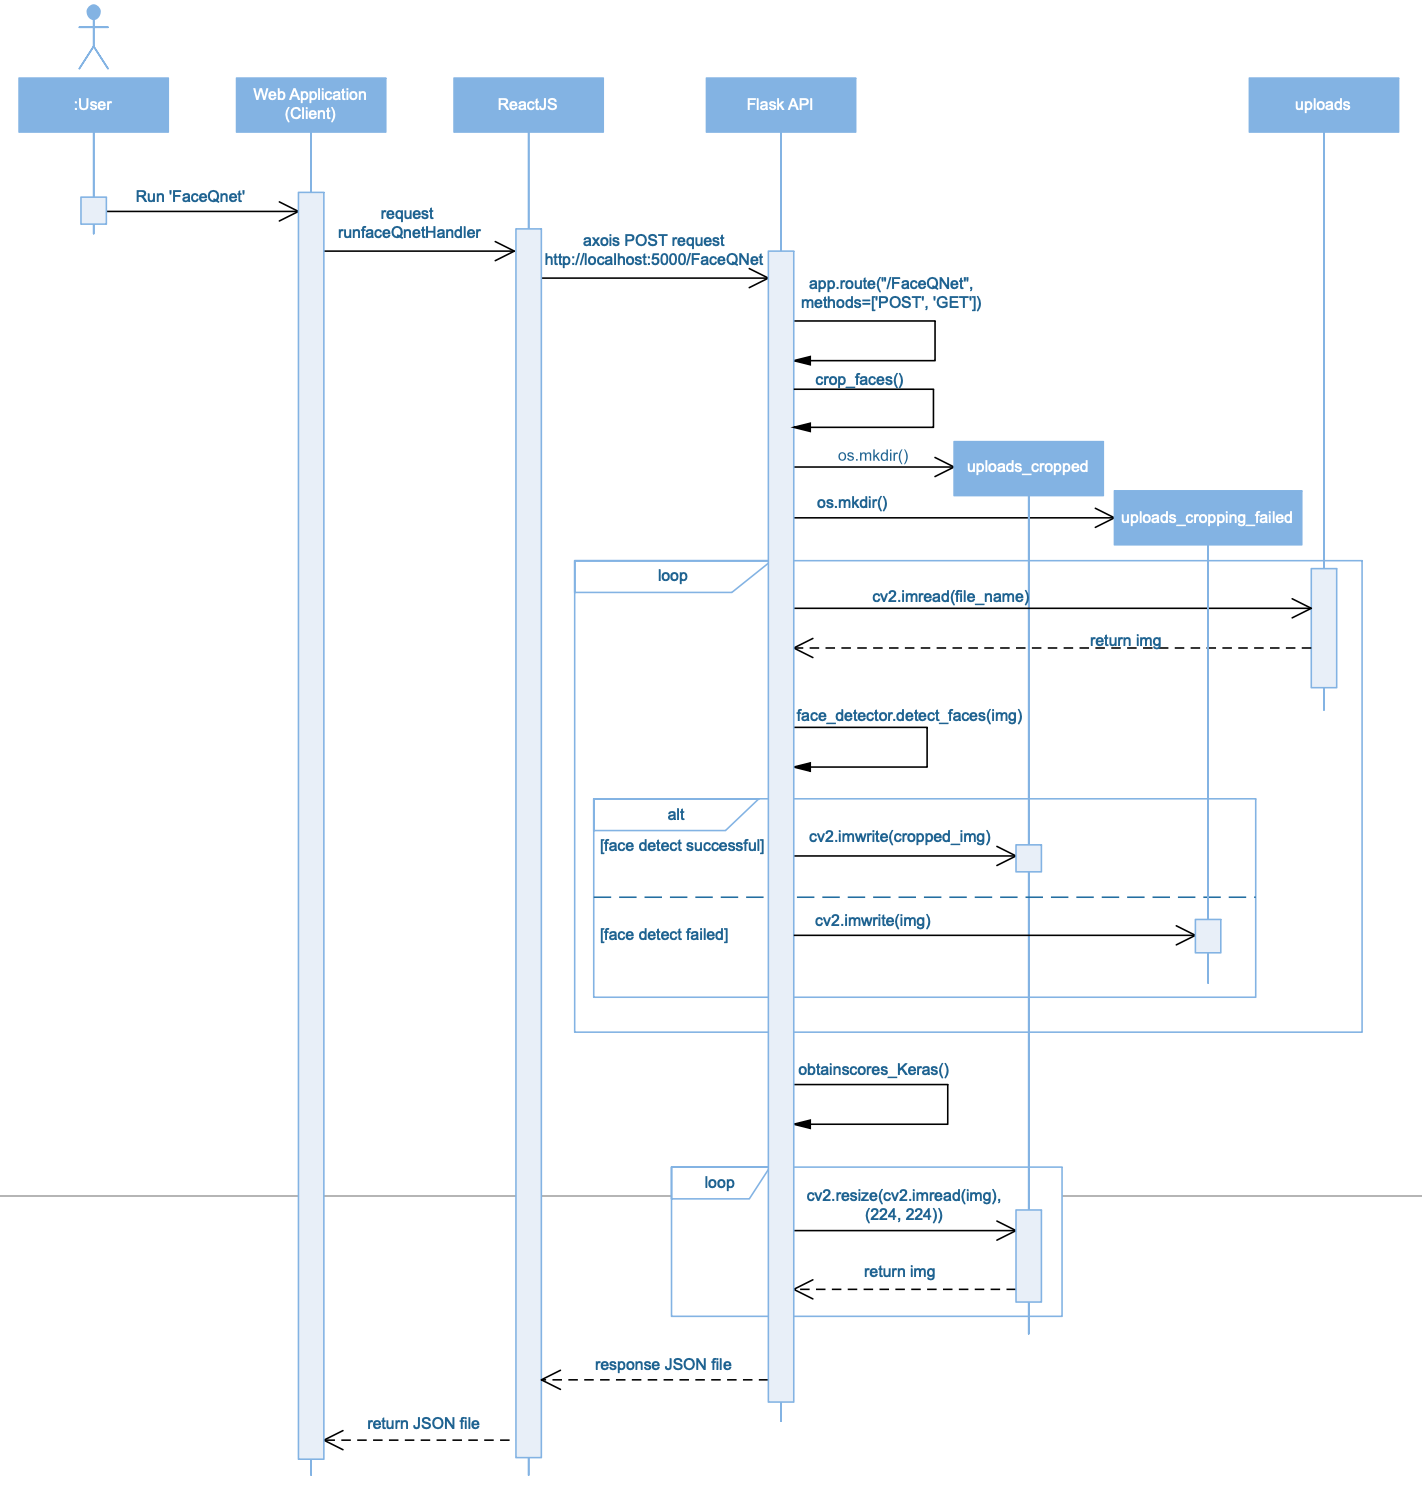
\includegraphics[width=1\textwidth]{figures/FerdigLowLevel.png}
    \caption{FaceQnet: low level sequence diagram.}
    \label{fig:lowlevel}
\end{figure}

The cropping phase of FaceQnet begins, and since this is the first time the API has been called, two folders by the name of ``uploads\_cropped'' and ``uploads\_cropping\_failed'' are created. The function then enters a for-loop that reads all the uploaded images from the original ``uploads'' folder, before they are cropped. Unfortunately, the cropping tool provided by MTCNN sometimes fails to detect the face in the images which results in an empty image. An alternative scenario then occurs, which sends these images to ``uploads\_cropping\_failed'', and they will automatically be provided with the lowest score possible. If no exception happens during the face cropping, the cropped image is saved to the ``uploads\_cropped'' folder. After having finished the cropping, the API starts the scores calculation, which first has to read all images from ``uploads\_cropped'', resize them and then calculates their scores. The metric likewise returns a JSON file with all scores back to the web page.

\section{Testing}
\label{sec:testing}
Before we finalized the development of the web application, it was important to have the users and the product owner test the product and provide their feedback. 

\subsection{User Testing}
We began the user testing at the end of the development process. The user testing was done by the product owner. Since the target group of the web application was a small number of users at Mobai, the product owner was a perfect representation of the group. While this might initially sound limited we have to keep in mind that the application created is targeted for a small number of users at Mobai and the product owner will be a perfect representation of the users of our application. The testing began after the user received an email with a link to the Github repository containing the source code of the web application. The email also included a list of tasks for the user to complete and a few questions about the user experience. The tasks and questions are listed in Table \ref{table:usertesttasks} and \ref{table:usertestquestions}. The user testing was discussed with the product owner during our next meeting to expand upon the feedback we received. If there was no comment on the task or question, the feedback was set as ``satisfactory''. The required changes were implemented as described in Table \ref{table:userTestIssues}.

\begin{table}[h]
%\centering
\caption{Issues and solutions following the user testing.}
\resizebox{\textwidth}{!}{%
\begin{tabular}{|p{7.5cm}|p{7.5cm}|p{1cm}|} 
\hline
\textbf{Issue} & \textbf{Solution} & \textbf{Status}  \\ \hline
Headings in the web application have line breaks.
&
Edit the width of the React component from small to medium.
&
Done
\\ \hline
When the metrics are running in the backend, there is no text telling the user what is going on.
&
Add a text field next in the code next to the loading circle with the current status.
&
Done
\\ \hline
The scores from the metrics have too many decimals. Change this to four decimals.
&
Add the round() function with four decimals to the metric scores.
&
Done
\\ \hline
The ``Delete'' button should be on the right side of the ``Upload'' button
&
Move the code for the ``Delete'' button to the correct position.
&
Done
\\ \hline
The attribute results from FaceQnet should not be set to zero.
&
Fix the code so that the attribute results from FaceQnet are set to -1. Add a text field explaining that -1 means that it does not return a score.
&
Done
\\ \hline
\end{tabular}%
}
\label{table:userTestIssues}
\end{table}


\begin{table}[h]
%\centering
\caption{User testing tasks and feedback.}
\resizebox{\textwidth}{!}{%
\begin{tabular}{|p{11cm}|p{3cm}|} 
\hline
\textbf{Task} & \textbf{Feedback}  \\ \hline
Launch the frontend and the backend on the users' computers using Docker.
&
Satisfactory
\\ \hline
Upload multiple images to the backend from the users' computers using the frontend.
&
Satisfactory
\\ \hline
Run all metrics at the same time with the images uploaded in the second task.
&
Satisfactory
\\ \hline
Run each of the metrics separately with the images uploaded in the second task. 
&
Satisfactory
\\ \hline
Delete the images uploaded to the backend.
&
Satisfactory
\\ \hline
Upload a single image to the backend from the users' computers using the frontend.
&
Satisfactory
\\ \hline
Run all metrics at the same time with the image uploaded in the sixth task.
&
Satisfactory
\\ \hline
Run each of the metrics separately with the image uploaded in the sixth task.
&
Satisfactory
\\ \hline
\end{tabular}%
}
\label{table:usertesttasks}
\end{table}

\begin{table}[H]
%\centering
\caption{User testing questions and feedback.}
\resizebox{\textwidth}{!}{%
\begin{tabular}{|p{5cm}|p{9cm}|} 
\hline
\textbf{Question} & \textbf{Feedback}  \\ \hline
How is the visual design?
&
The design looks good enough. Designers can update it later to make it better.
\\ \hline
Is the user interface intuitive?
&
The user interface is simple and easy to understand.
\\ \hline
Are the metric results displayed in a satisfying way?
&
Cut down the precision of the scores from the metrics down to four decimals.

FaceQnet does not return any attribute scores and instead sets them to the number zero. This can create misunderstandings for the users. Change this to the text ``None''. Another solution is to set the score to the number minus one and add the text ``-1 indicates this approach does not return a score'' to the frontend.    
\\ \hline
Any other feedback about the user experience?
&
A loading circle is shown when the metrics are working in the backend. Add the text ``Processing is ongoing'' to let the user know what is going on.

The ``Delete'' button is located to the left of the ``Browse Files'' button. Move this to the right side of the ``Upload'' button.

Some of the text in the headers of the web application is wrapping to a new line. Keep it on the same row.
\\ \hline
\end{tabular}%
}
\label{table:usertestquestions}
\end{table} 
\chapter{Subjective Experiment}

%- Why do we need ground truth data
%- introduce datasets
%- what is a subjective experiment?
%- Conduct subjective experiment to collect ground truth data

\label{chap:subjective}
This chapter contains the process of designing and conducting our subjective experiments. In Section \ref{sec:groundTruth} we explain how and why collecting ground truth data is important in this project. The next Section \ref{sec:SubjectiveAspects} addresses important aspects when creating a subjective experiment. These sections are followed by the introduction of datasets used in the experiment and application (Section \ref{sec:datasets}) as well as an in-depth description of our subjective experiment in Section \ref{sec:OurSubjectiveExperiment}. At the end of this chapter we introduce the creation of our own dataset in Section \ref{sec:ownData} followed by our second subjective experiment in Section \ref{sec:secondse}.

\section{Why Collect Ground Truth Data?}
\label{sec:groundTruth}
Ground truth data is data based on human assessments. The ground truth data is collected by arranging subjective experiments where human observers are asked to evaluate a set of images according to given criteria \cite{Xphdthesis}. In this project, observers graded facial images. Gathering ground truth data is an essential part of our work, because subjective data is needed to evaluate the performance of the objective assessments. Validation between subjective and objective assessments ensure whether the FIQMs correspond with how human observers rate facial images. 

\section{Subjective Experiment Aspects}
\label{sec:SubjectiveAspects}
As mentioned in Section \ref{section:academic background}, our lack of experience indicated that an introduction to subjective experiments was needed. The research about this topic made us realize the importance and difficulties with this task. There were several assessments to perform in terms of creating a comprehensive subjective experiment such as type of psychophysical experiment, duration of experiment and observer types.

\subsection{Experiment Method}
There were several psychophysical experiment methods to choose. We based our choice on the method that fitted our experiment the best. The options were between category judgment and rank order. Category judgment is a method where the observers rate facial images based on given criteria. These images are allocated to a category \cite{Xphdthesis}. In rank order the observers are shown multiple images simultaneously and asked to rank them according to each other. 

\subsection{Experiment Duration}
The experiment duration is an important factor when conducting a subjective experiment. On the one hand, it is essential to give the observers a high number of facial images to grade for data collecting purposes. On the other hand, having a too long experiment can cause observer fatigue such as eye fatigue or headache. These kinds of disorders will affect the subjective data negatively.

\subsection{Observers}
The subjective experiment was available for everyone to perform, but we invited a specific target group that works in this field. The observers were divided in two groups: experts and non-experts.

\subsubsection*{Experts}
The experts are people who were specially invited to complete the experiment. These observers work either for Mobai with facial recognition systems or at NTNU in the Faculty of Information Technology and Electronics. A point of having experts in the field doing the subjective experiment was to quality assure our creation since they to a larger degree can distinguish between quality issues. In addition to that, we were to compare the results between the two groups. 

\subsubsection*{Non-experts}
Non-experts were people with no experience in the biometric field. They were our friends and family of different ages and educations.

\section{Datasets}
\label{sec:datasets}
The usage of facial images in the application and subjective experiment raised GDPR issues. It would strike against the rules if we photographed people on the streets or collected random images on the web without consent from the subjects. The ground truth data in this project was collected on three different datasets provided by Mobai. Table \ref{table:DatasetInformation} displays all datasets used in the project. Combined passport alike was a high resolution dataset with images from the Tufts Face Database \cite{Tufts-Face-Database} and FEI Face Database \cite{FEI-Face-Database}, which has a similarity to passport or id photos, hence the title. The set consisted of 98 facial images of people with different poses, facial expressions and lighting. All images were taken using a Nikon D3100 with a dark blue or light grey background, as depicted in Figure \ref{fig:combined_passport_alike}. The camera distance was equal in every photo and the camera lens was in an even height with the faces. 

% \begin{figure}[h]
%     \centering
%     \subfloat[\centering]{{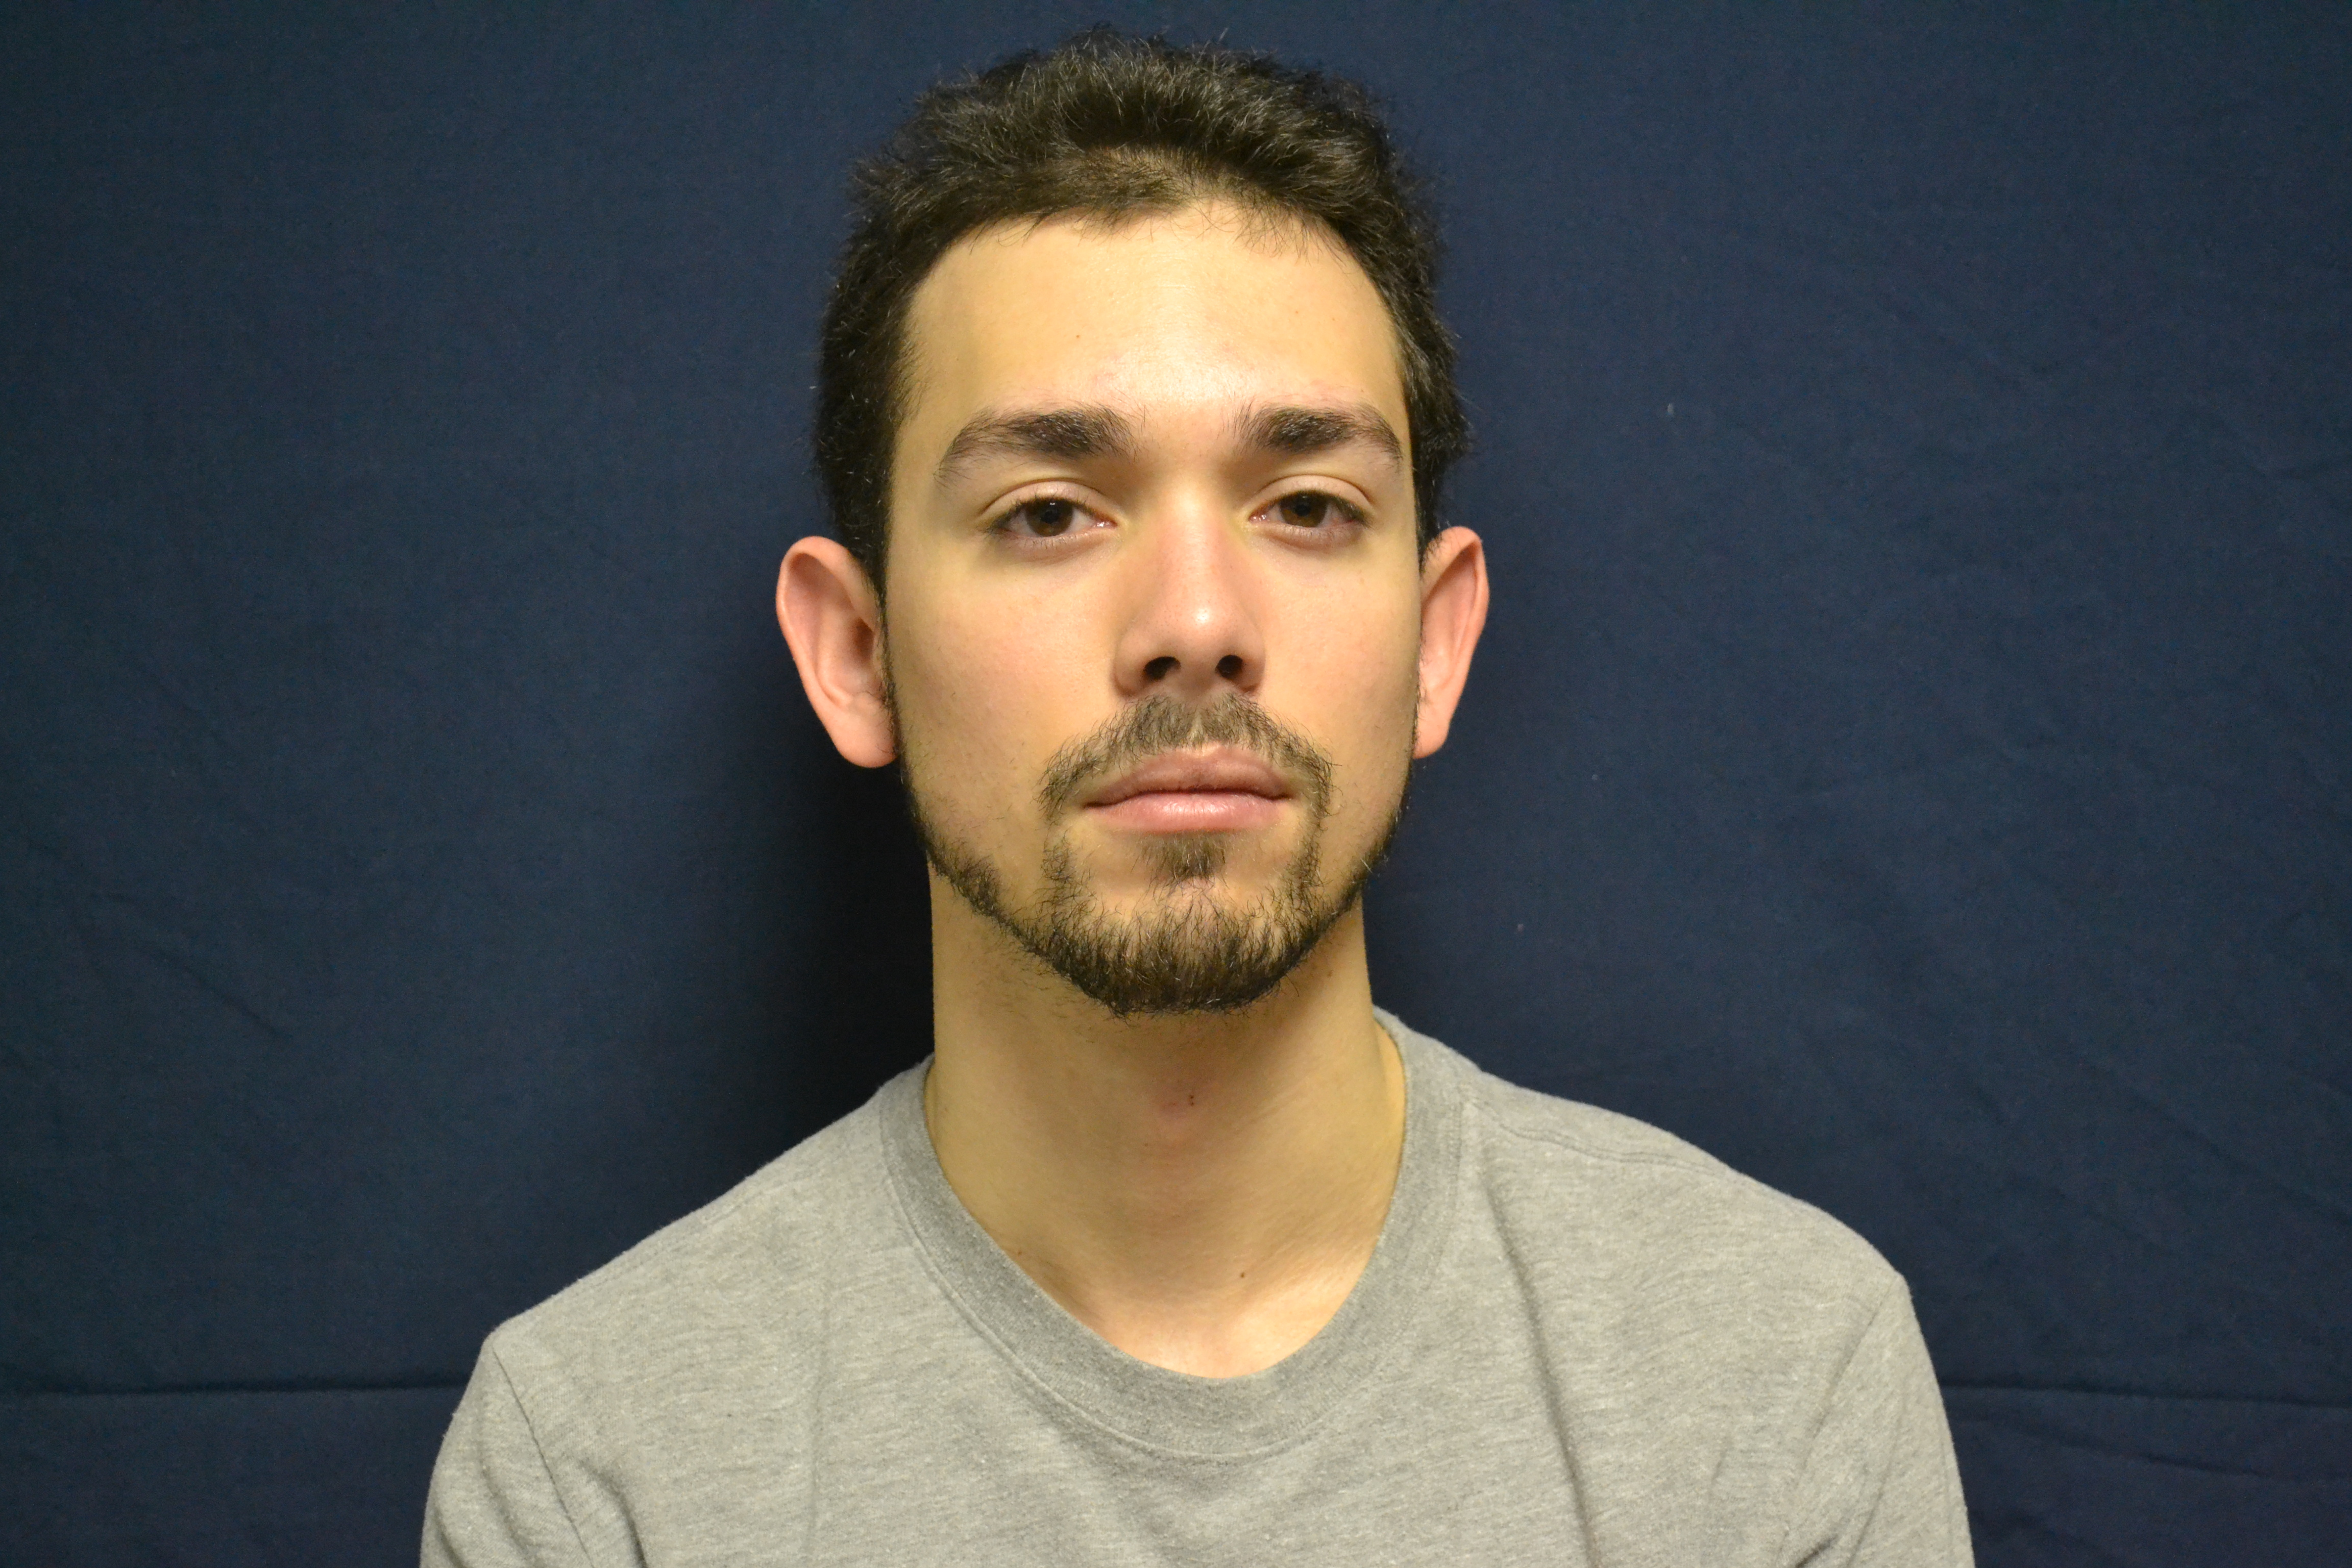
\includegraphics[width=4.1cm]{figures/0.jpg} }}
%     \qquad
%     \subfloat[\centering]{{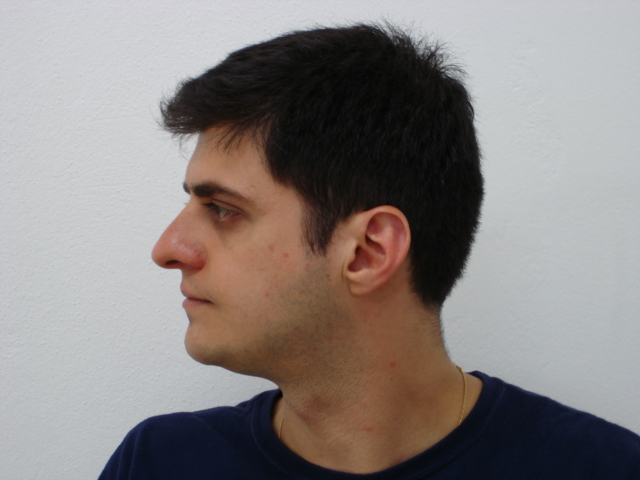
\includegraphics[width=3.65cm]{figures/50.jpg} }}
%     \caption{Facial images from Combined passport alike.}
%     \label{fig:combined_passport_alike}
% \end{figure}
%
\begin{figure}[h]
\centering
    \subfloat
        {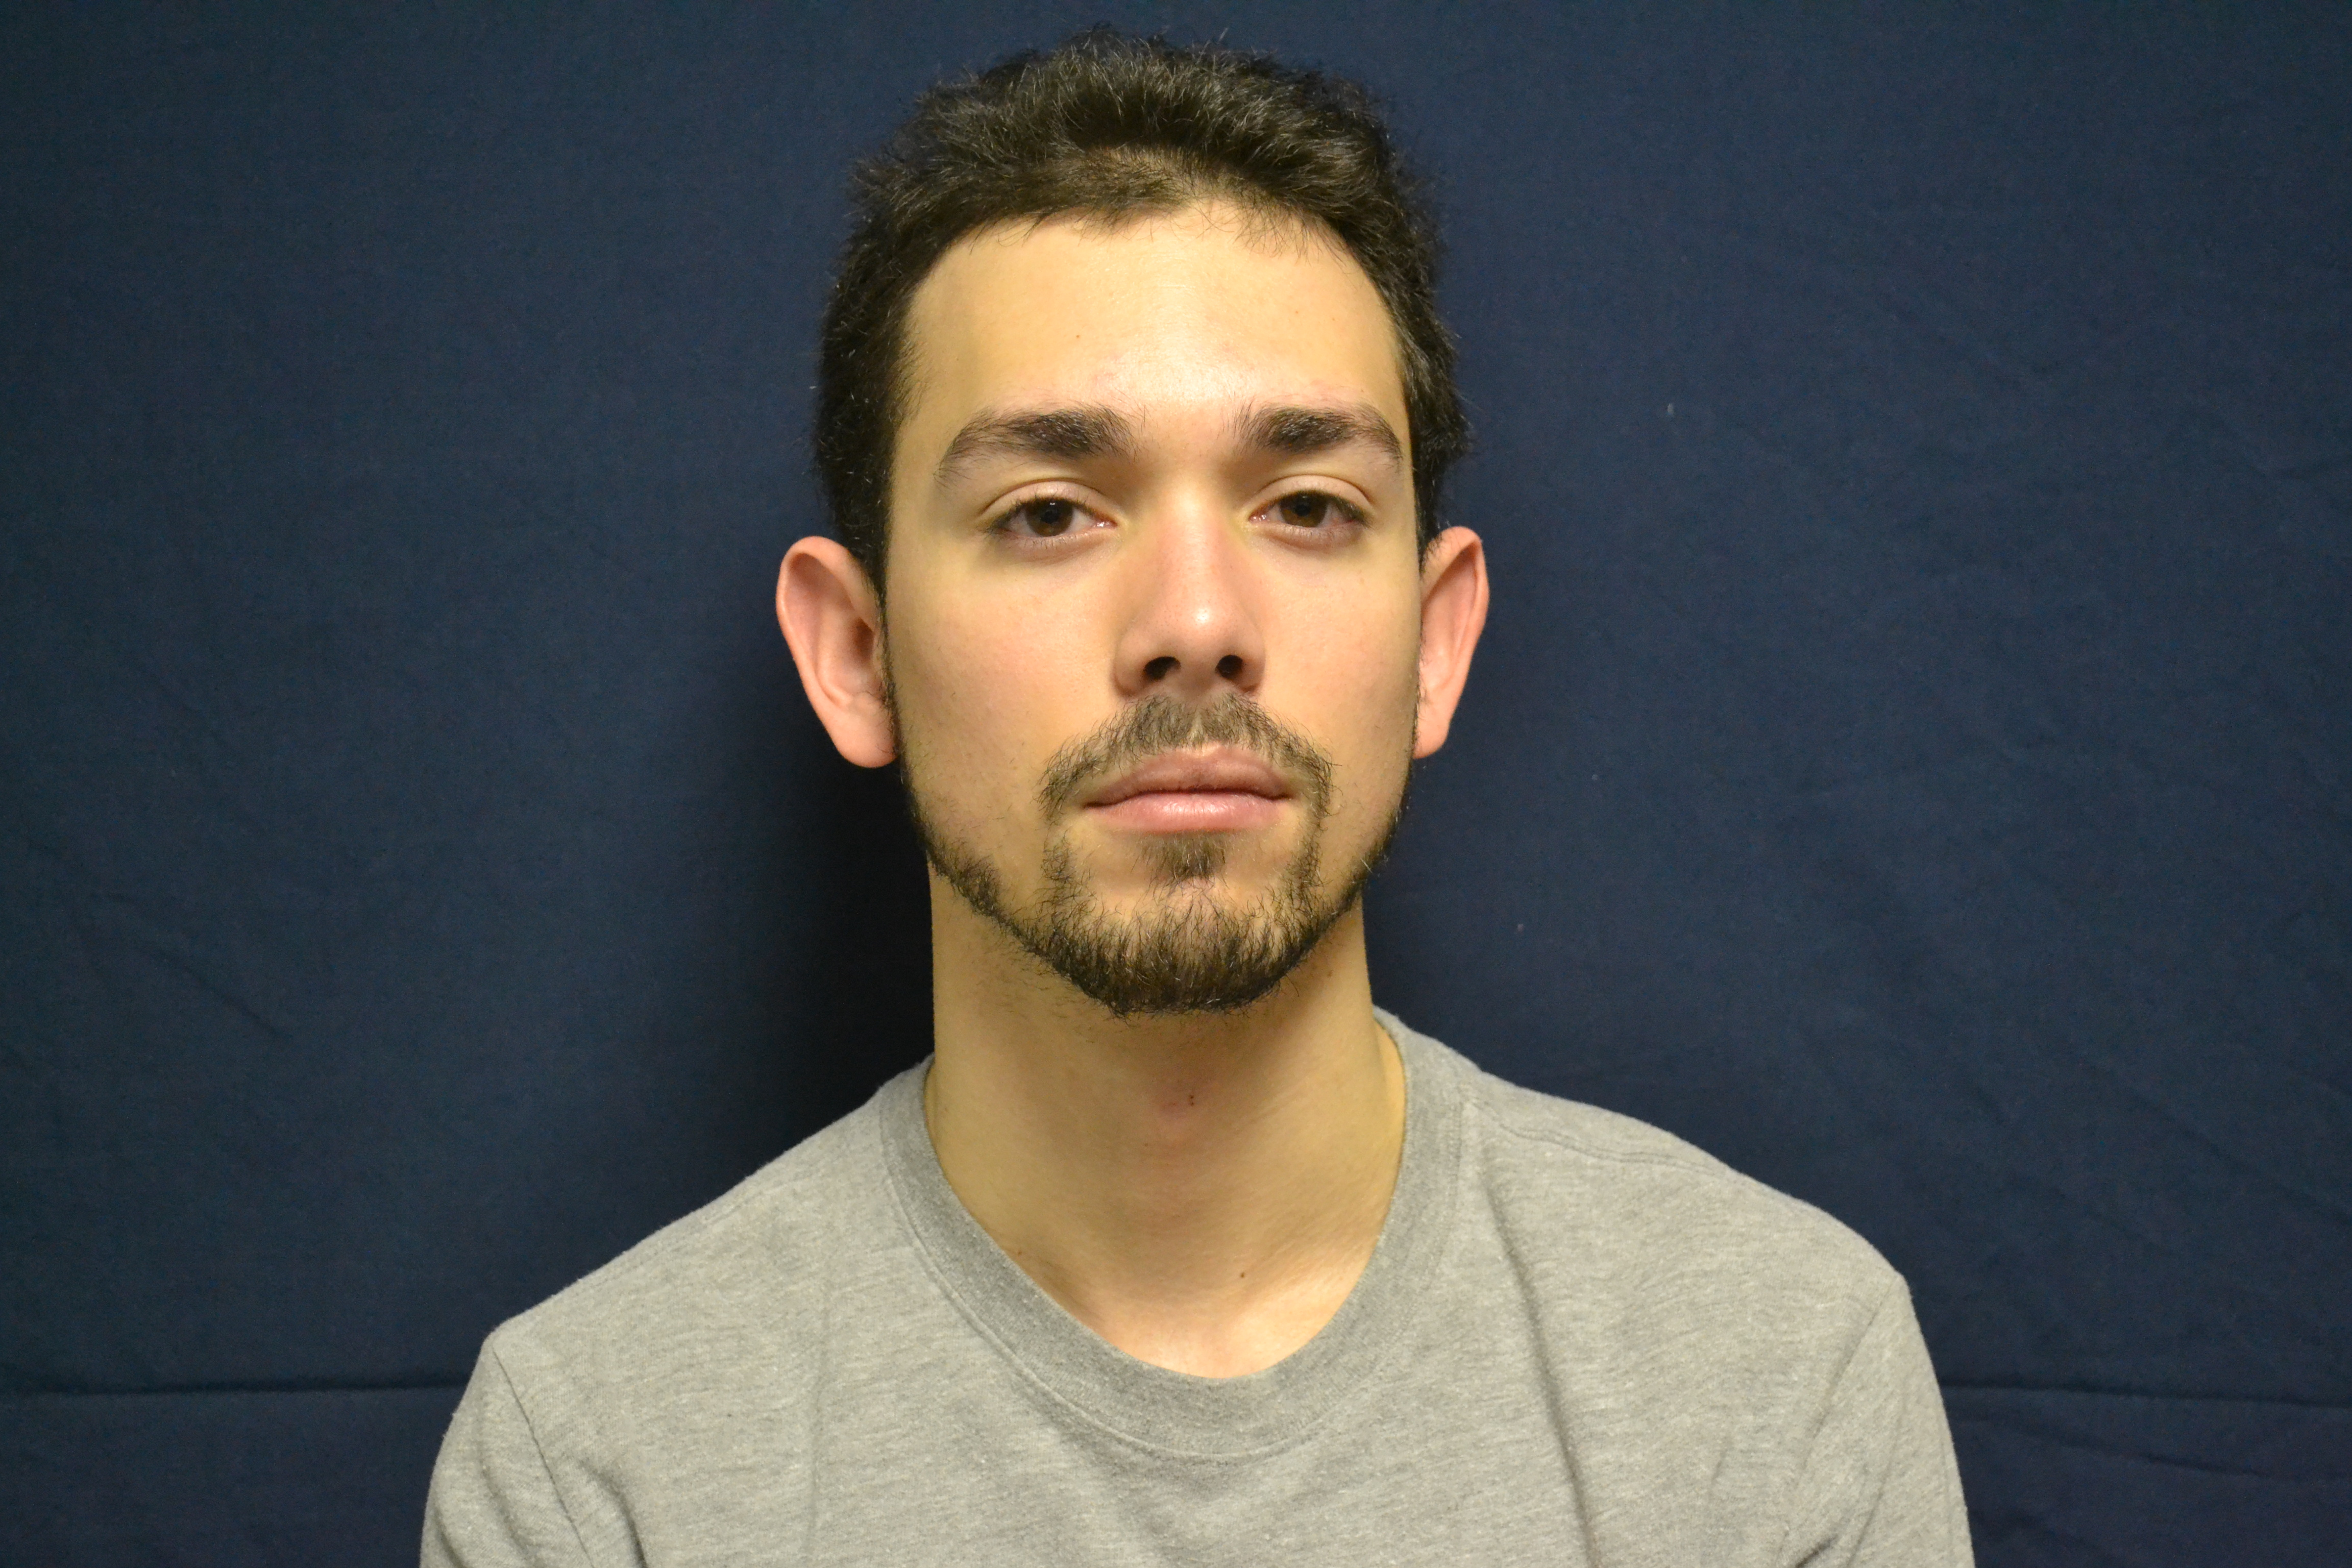
\includegraphics[scale = 0.12]{figures/0.jpg}\hspace{0.42cm}}
    \subfloat
        {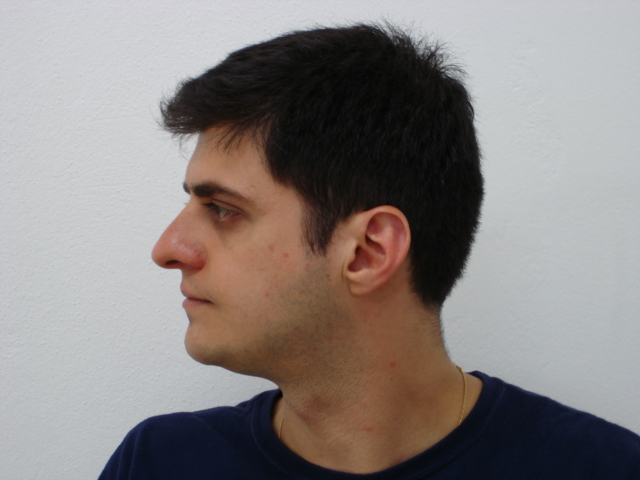
\includegraphics[scale = 0.185]{figures/50.jpg}\hspace{0.42cm}}
    \caption{Facial images from Combined passport alike.}
    \label{fig:combined_passport_alike}
\end{figure}
%
Capture from photo was created by several employees at NTNU and combined with images from the CASIA Face Antispoofing Database \cite{CASIA-FAD}. All 70 images were selfies, taken with different phone cameras. Like Combined passport alike, the people had different poses and facial expressions. However, in this dataset, the images by the NTNU employees were photographed in multiple locations on campus, which made the background and lighting vary considerably. The CASIA images were captured from computer screens that would possibly affect the FIQM's evaluation scores. Due to GDPR issues, only images from CASIA are included in Figure \ref{fig:capture_from_photo}.
%
% \begin{figure}[h]
%     \centering
%     \subfloat[\centering]{{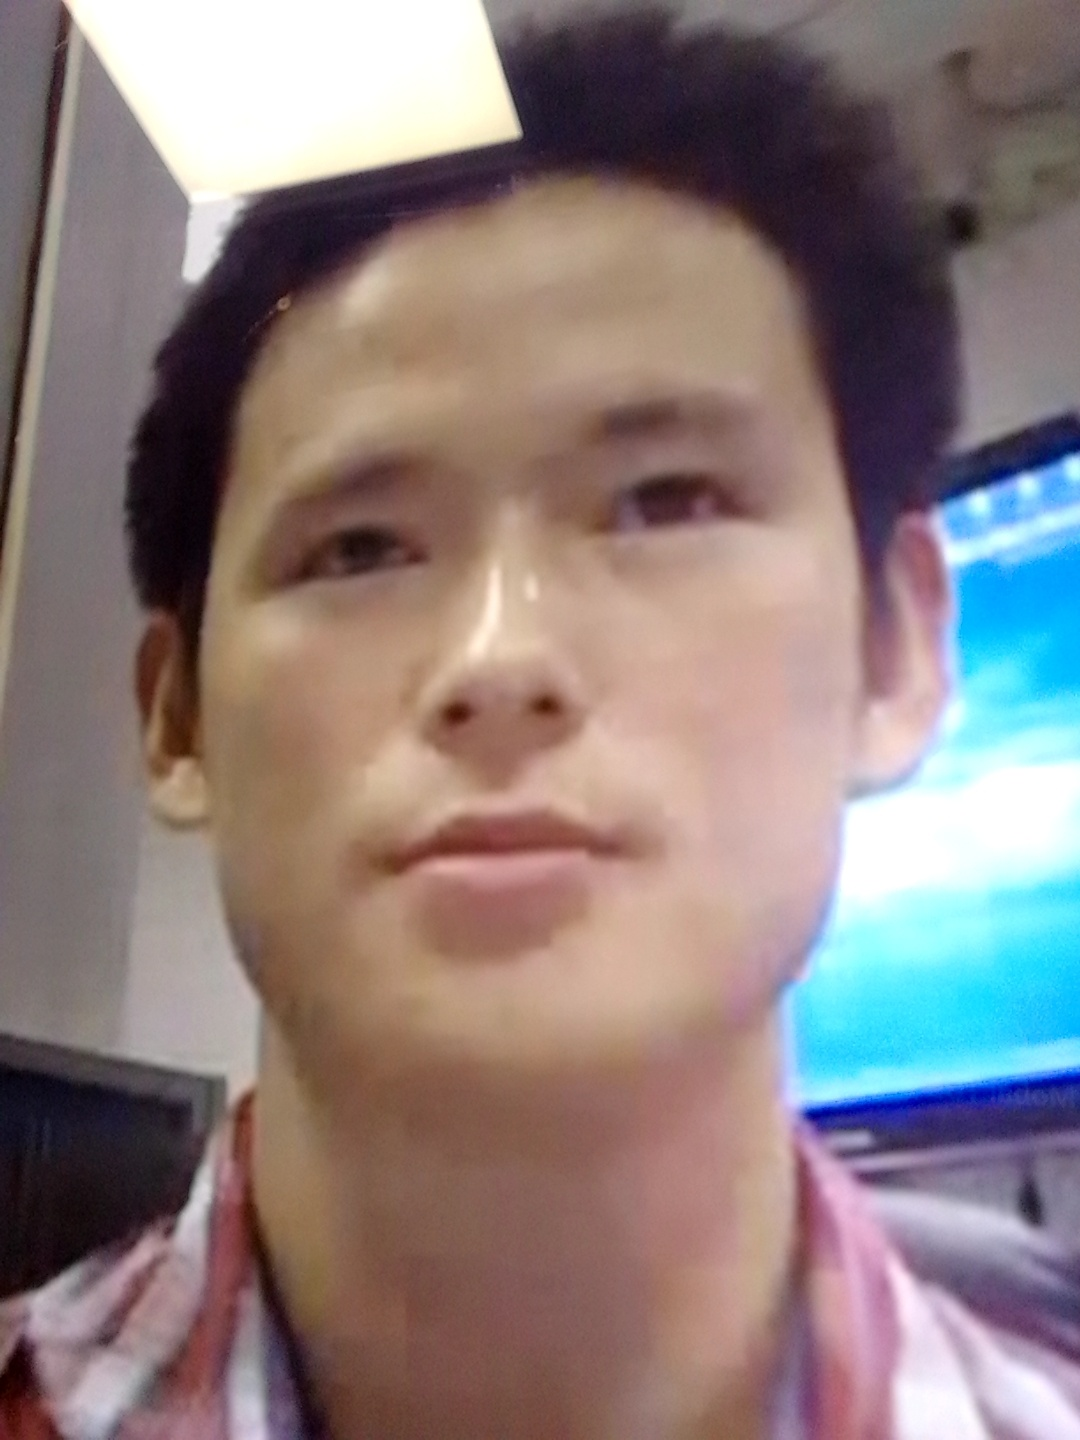
\includegraphics[width=3cm]{figures/1_0.89185.jpg} }}
%     \qquad
%     \subfloat[\centering]{{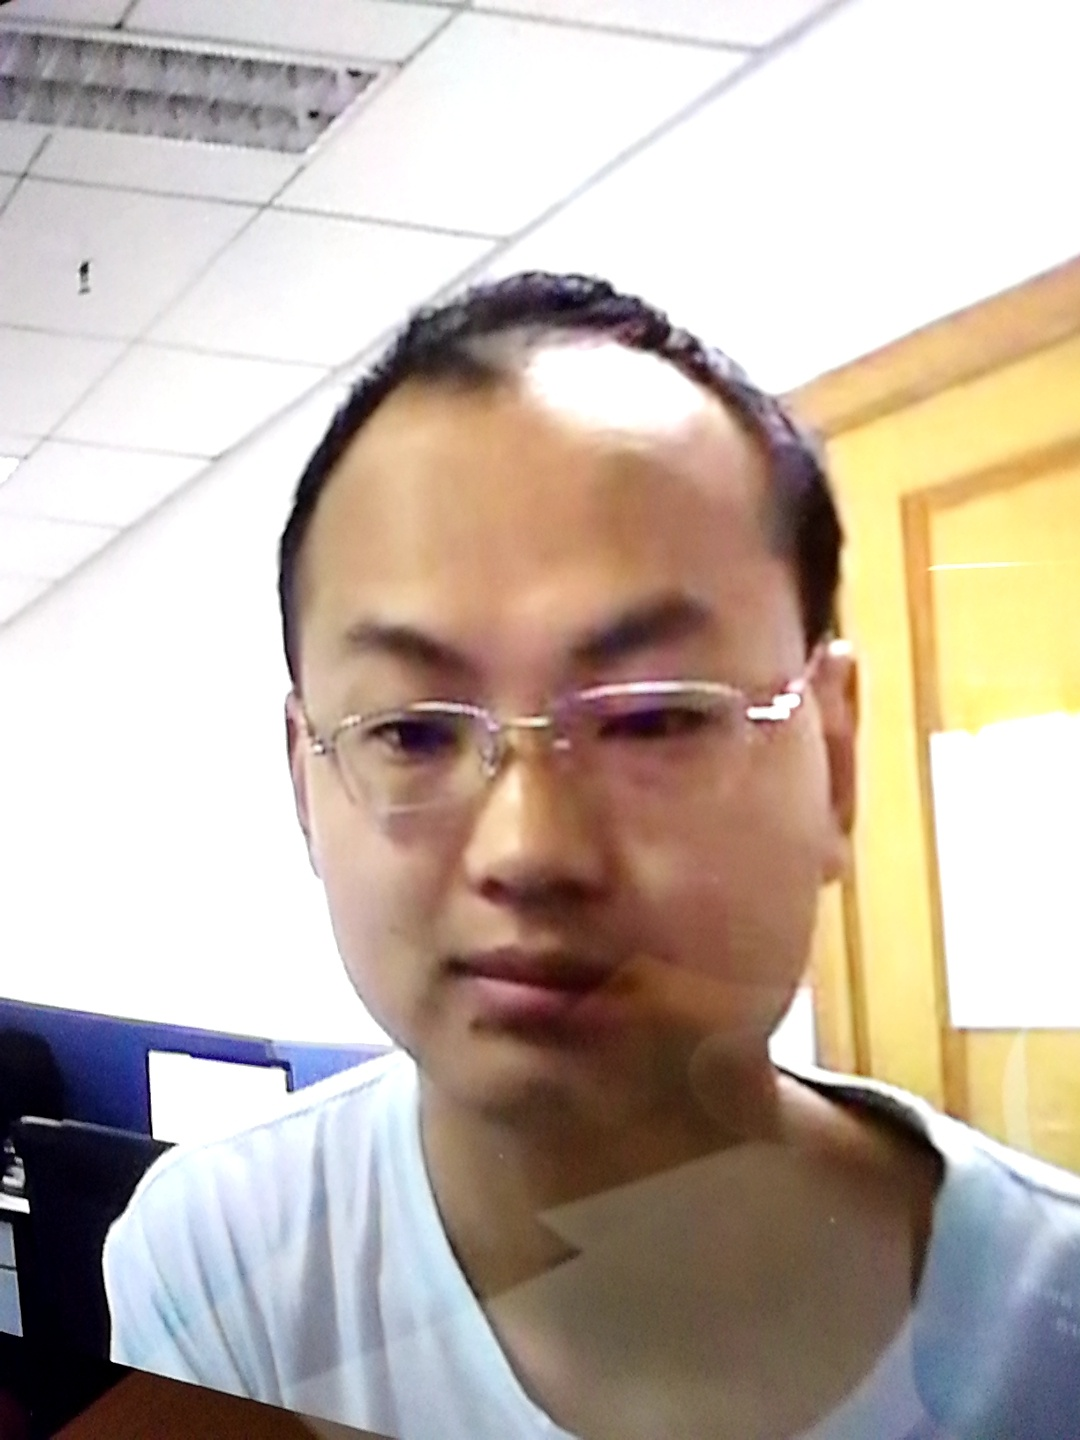
\includegraphics[width=3cm]{figures/5_0.97369.jpg} }}
%     \caption{Facial images from Capture from photo.}
%     \label{fig:capture_from_photo}
% \end{figure}

\begin{figure}[h]
\centering
    \subfloat
        {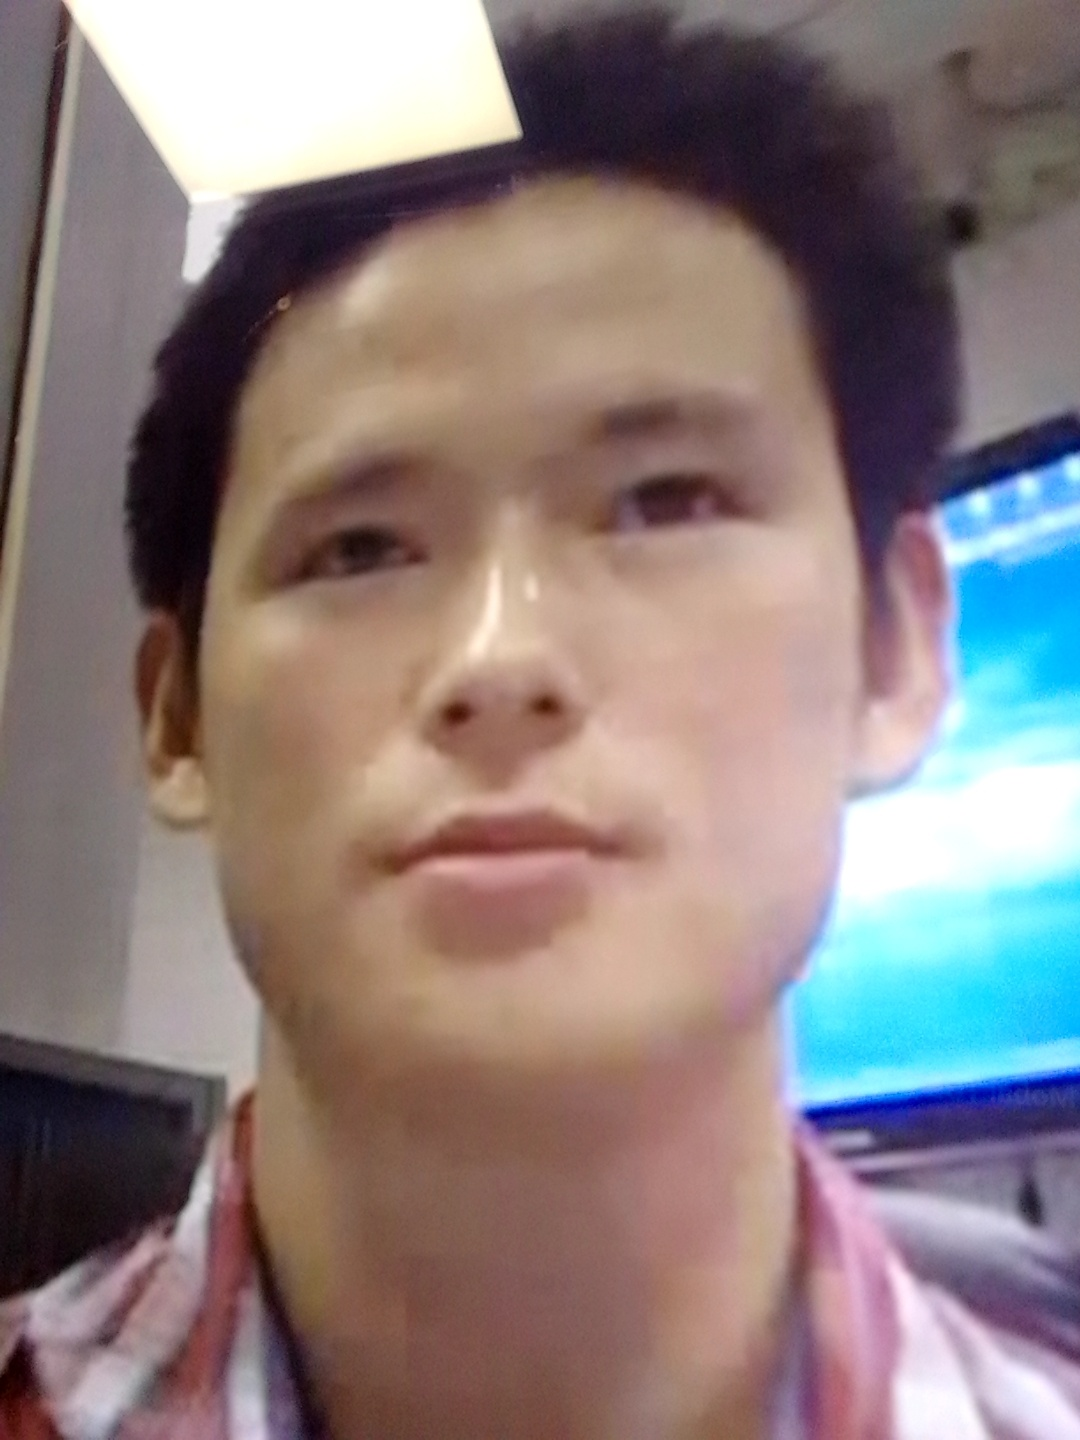
\includegraphics[scale = 0.09]{figures/1_0.89185.jpg}\hspace{0.42cm}}
    \subfloat
        {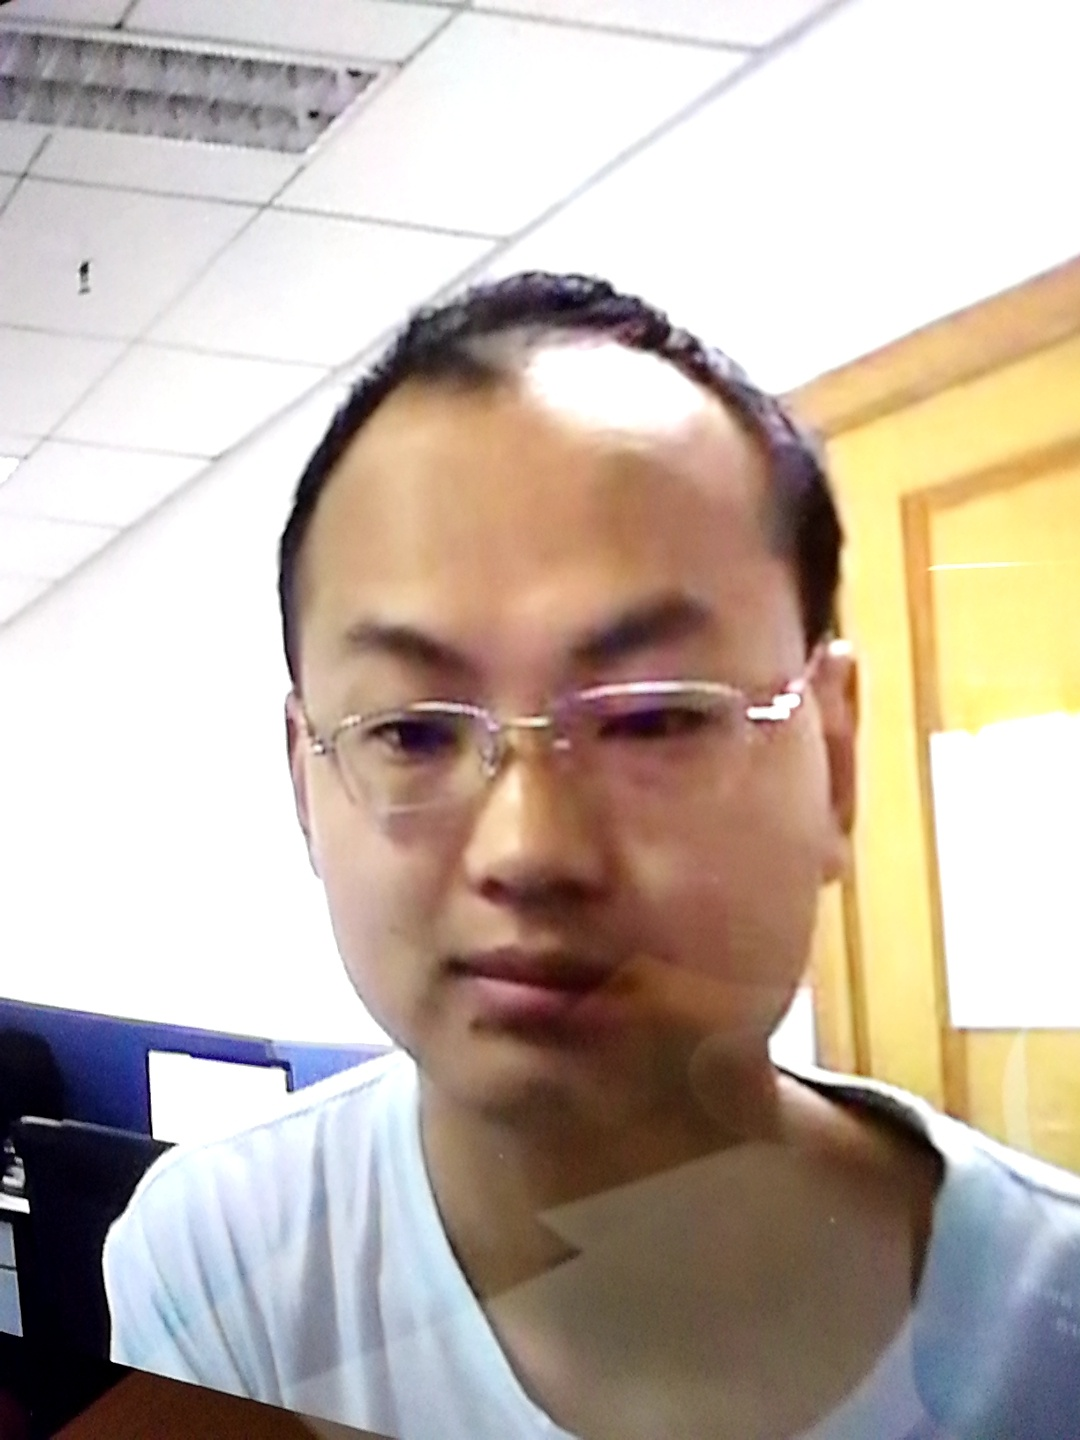
\includegraphics[scale = 0.09]{figures/5_0.97369.jpg}\hspace{0.42cm}}
    \caption{Facial images from Capture from photo.}
    \label{fig:capture_from_photo}
\end{figure}
%
The Selfie dataset was a set of 126 images accessible on the web \cite{selfie-dataset}. The images were selfies of different people at numerous locations: both indoors and outdoors. Given the selfies, the photos were taken with phone cameras and the camera to subject distance was short. A sample from the dataset is shown in Figure \ref{fig:selfie_dataset}. 
%
% \begin{figure}[h]
%     \centering
%     \subfloat[\centering]{{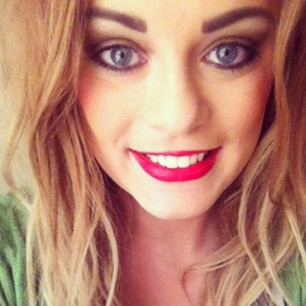
\includegraphics[width=3cm]{figures/10249165_693227110715964_1497214365_a.jpg} }}
%     \qquad
%     \subfloat[\centering]{{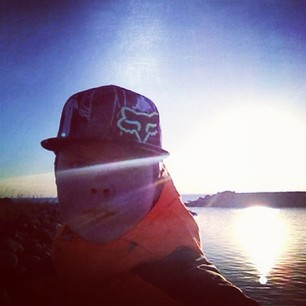
\includegraphics[width=3cm]{figures/10251439_436588196485138_396348425_a.jpg} }}
%     \caption{Facial images from Selfie dataset.}
%     \label{fig:selfie_dataset}
% \end{figure}
\begin{figure}[h]
\centering
    \subfloat
        {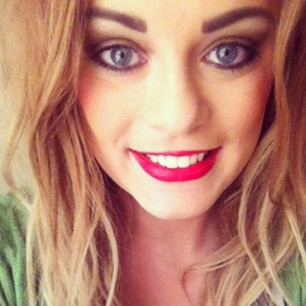
\includegraphics[scale = 0.3]{figures/10249165_693227110715964_1497214365_a.jpg}\hspace{0.42cm}}
    \subfloat
        {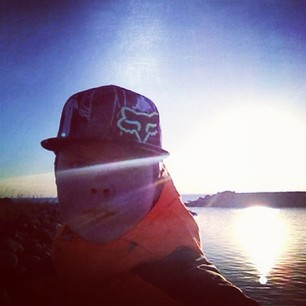
\includegraphics[scale = 0.3]{figures/10251439_436588196485138_396348425_a.jpg}\hspace{0.42cm}}
    \caption{Facial images from Selfie dataset.}
    \label{fig:selfie_dataset}
\end{figure}

%\newpage

\begin{table}[h]
\caption{Information about all datasets used in the project.}
\resizebox{\textwidth}{!}{%
\begin{tabular}{|p{4cm}|p{4cm}|p{4cm}|p{4cm}|} 
\hline
\textbf{Dataset name} & \textbf{Number of images} & \textbf{Captured with} & \textbf{Distortions}  \\ \hline
Combined passport alike & 98 & Nikon D3100 & Exposure \\ \hline
Captured from photo & 70 & Mobile phone & N/A \\ \hline
Selfie dataset & 126 & Mobile phone & N/A \\ \hline
Norwegian Facial Collection (Section \ref{sec:ownData}) & 450 & Apple Iphone 8 \newline Apple Iphone 11 \newline Motorola Moto G5S Plus & Compression \newline Blur  \newline Noise \newline Face mask coverings \newline Oblique angles \\ \hline
\end{tabular}%
}
\label{table:DatasetInformation}
\end{table}

\section{Our Subjective Experiment}
\label{sec:OurSubjectiveExperiment}
In our subjective experiment we used category judgment. The observers were asked to grade facial images according to the criteria described in Section \ref{sec:intromanual}, and assign these images in five categories: poor, bad, fair, good and excellent. We did not chose the rank order system, because comparing multiple images would be challenging and time consuming for the observers. The experiment was separated into three sessions with a five-minute time break between each session. The duration of the subjective experiment was estimated to take approximately 45 minutes. Each session included images from the three datasets which were equally distributed among the sessions. For us, it was important to randomize the facial images to prevent observers getting biased towards one face. The subjective scores were collected from 15 observers - both experts and non-experts. Due to the GDPR, we only asked the observers' gender and if they were experts or not in this field. Out of the 15, 13 were men and two were women. Seven observers were experts, and eight were non-experts. Six experts were men, and one woman. Seven non-experts were men, and one non-expert was a woman. 
%
\subsection{Instruction Manual}
\label{sec:intromanual}
When conducting the subjective experiment and collecting the ground truth data, we first needed to provide a detailed instruction to the observers. This was especially important in the case of non-experts who were not familiar with the task. Such an instruction manual will also allow us to provide a uniform understanding for the observers on how they should perform the subjective experiment. Thus, an experiment instruction manual was created. The instruction manual is included in Appendix \ref{app:survey-instructions} 

The first clarification we had to convey to the participants, was the meaning of face image quality. Both experts and non-experts would have different perceptions in terms of face image quality and we had to clarify all factors affecting the quality. The most clear and effective way to train the observers was to visualize examples of rated images like they would do in the subjective experiment. We created five example lineups with selfies of ourselves. Those lineups included most issues affecting the quality of an image. 

\begin{figure}[h]
\centering
    \subfloat[Poor]
        {
\includegraphics[scale = 0.0825]{figures/lineup1.png}}
    \subfloat[Bad]
        {
\includegraphics[scale = 0.0901]{figures/lineup2.png}}
    \subfloat[Fair]
        {
\includegraphics[scale = 0.0825]{figures/lineup3.png}}
    \subfloat[Good]
        {
\includegraphics[scale = 0.09]{figures/lineup4 - Copy.png}}
    \subfloat[Excellent]
        {
\includegraphics[scale = 0.0825]{figures/lineup5.png}}
    \caption{A lineup from the experiment instruction manual and their quality ratings.}
    \label{fig:example-manual}
\end{figure}

The images in Figure \ref{fig:example-manual} is a sample lineup provided to the observers to guide them on how to rate the images. In the experiment however, some participants found it harder to rate the experiment images, because they included several image properties to take into account.

\subsection{Choice of Subjective Experiment Platform}
\label{subsection:choicesoftware}
A decision we thought would be easy, but ended up being challenging and time consuming was selecting the platform in which we would run our subjective experiment. There were a number of possible platforms for conducting the subjective experiment. However, we had to bare in mind the factors described in Section \ref{sec:SubjectiveAspects} in our selection. One experiment platform we found interesting was Survey Monkey. The main reason we abstained from Survey Monkey was their demand of creating a yearly subscription to use functions such as displaying questions in random order. We even asked for a four month subscription without luck. Another platform we found appropriate was Survey Legend, a subjective experiment platform perfectly suitable for images. It included many functions we needed, except enabling questions to be ordered randomly for each observer. Therefore, we unfortunately had to abort Survey Legend as well. 

After consulting with our supervisor, we ended up arranging the subjective experiment in QuickEval \cite{QuickEval} - an experiment platform developed by NTNU. The platform provided all functionality we needed such as category judgment and random order of questions. Each image was positioned in the center of the screen on a neutral background, we also took care that every image in the datasets were similar in size. QuickEval displayed statistics in the application gradually as people responded to the experiment. The statistics data was also downloadable as a CSV, HTML or Excel file. Using QuickEval as a experiment platform ended up being a good choice because it was created by NTNU and we had a close relationship with the developers. When an issue occurred, we submitted that issue and communicated directly with a developer, resulting in the issue to be fixed quickly. 

\section{COVID-19 Pandemic Implications}
Due to the ongoing COVID-19 pandemic, limitations with the subjective experiment occurred. For example, we did not have the opportunity to create a controlled environment and invite the participants to complete the subjective experiment there. Ideally, such a controlled environment would be a well-lit room with good air quality, timed breaks between the sessions and a computer with specific screen settings for all participants to complete the experiment on. The Norwegian Colour and Visual Computing Laboratory in NTNU Gjøvik would be a perfect environment that could be standardized according to \acrfull{cie} publications, but unfortunately this was not achievable given the COVID-19 restrictions. For that reason, all the participants completed the subjective experiments in an uncontrolled environment using their own computers with their custom screen resolution and lighting conditions. While factors such as the monitor brightness and color temperature and even the participants distance from the monitor as well as the illuminance of the room, plays an important role. We believe that due to the nature of our experiment (collecting ground truth data) the results collected in our work would be reliable and scientifically accurate. We should point out that while when it comes to evaluating the general quality of the image parameters such as the viewing condition and/or emotions of the observers play an important role this is normally not the case in the type of subjective data we were collecting. 

\raggedbottom %Fikser problemer med white space

\section{What Went Wrong?}
Despite conducting the subjective experiment in uncontrolled environments, the accomplishment of the experiment was successful. Due to the targeted invitation we sent to observers, a reasonable number of participant provided us with their subjective evaluation in a short time which resulted in us having more time analyzing the data. Since it was our first time creating this kind of experiment, some experiment aspects were left out of the consideration that could be important. The main flaw with this experiment was the lack of information about observes' characteristics, especially color blindness. Research show that \acrfull{cvd} affects eight percent of men and 0.5 percent of women in the world \cite{colorblindness}. Given that 87 percent of the observers participating in our experiment were men, there was a possibility that color blindness existed among the observers. People with a type of color blindness have the ability to discern colors to a lesser degree than people with normal color vision. Therefore, this will affect the way they assess the facial images, which is the reason why they are not contemplated as optimal observers \cite{Xphdthesis}. A good solution would be to test all participants with standardized color vision tests like an Ishihara test \cite{Ishihara} or a Cambridge color test \cite{CambridgeColorTest}.   

Another experimental aspect we systematically excluded was to provide the observers with a question during the experiment. We had initially planned for the experiment to consist of a precise question to minimize any doubt the observers could have. A criterion we had in mind was: ``How well is the face recognizable?''. We felt this question could confuse the observers given that the word recognize often refers to knowing a person in advance. Since most participants would not know any of the subjects in the datasets in advance, we dropped that question. However, since we created an instruction manual with aspects that affected the face quality, we figured the observers would have a clear understanding of what was to be rated. But looking back, a question like: ``How visible is the face according to the criteria described in the instruction manual?'', could have been beneficial to clear up any misunderstandings.   

\section{Creating Our Own Dataset}
\label{sec:ownData}
When working with machine learning and AI in the context of face recognition, the probability of using one of the famous pre-curated Labeled Faces in the Wild (LFW) datasets are highly likely. Conditions such as poor lighting, extreme poses and face coverings are somewhat lacking in LFW and these are all important aspects for Mobai´s face recognition system. This provided us with the opportunity to collect a specialized dataset designed to fit Mobai´s needs which led to the proposal of a new dataset. This initiative was positively received by Mobai.

The idea to collect a new dataset came about when the team was discussing flaws with the Selfie dataset. Mobai´s definition of face quality is, as mentioned in Section \ref{sec:setup}, originally based on ISO 29794-5 and ICAO Doc 9303 Part 3. Based on those definitions, one could argue that the images in the Selfie dataset did not fulfill the criteria. A significant part of the images in the Selfie dataset are of faces that either are way off-centered, too zoomed in or a combination of both. We figured it could be valuable for Mobai to have a new dataset aligned with certain criteria they valued. 

\subsection{Creation Process}
We had initially taken a few images of ourselves which were used for the instruction manual, illustrated in Figure \ref{fig:example-manual}, to the subjective experiment. These were included when we started collecting images for the dataset. We came to the conclusion that each day, starting 1. March and ending 15. April, we would capture at least five selfies of ourselves every day. This would result in a total of 250 images of each member. We ended up capturing 1172 images. With this amount of images, there were a lot of repetitive facial images. Therefore, we selected 250 images from the collection. In addition, we selected 50 of these images and added different distortions (described in detail in Section \ref{sec:secondse}) on them. The whole dataset ended up consisting of 450 images. Our dataset is relatively large in size in comparison to the datasets used in our experiment. Some of the images are similar to the Combined passport alike dataset in regards to pose, but our dataset includes several varieties and specialized conditions. We chose to name our data set Norwegian Facial Collection (NFC).

All images were captured using both the front and back camera of our mobile phones. This lead to our dataset containing images of varying resolution, given that our phones were not of the same type. The phones used for the dataset collection were:
\begin{itemize}
    \item Apple iPhone 8 
    \item Apple iPhone 11 (2 units)
    \item Motorola Moto G5S Plus 
\end{itemize}
%
These had different camera specifications with the front cameras ranging from seven to 12 megapixels and the back cameras ranging from 12 to 13 megapixels. While the difference in image resolution was very minor making it barely noticeable to the user, it still is able to simulate what FIQMs will need to address in real life applications. 

\subsection{Distortions}
Our dataset was inspired by the three datasets introduced in Section \ref{sec:datasets}, but was unique because elements like oblique angled images and face masks were represented. During our image collection, we gathered examples of our faces with: 
%
\begin{itemize}
    \item Different lighting conditions.
    \item Different facial expressions and head poses.
    \item Different face and head coverings. 
    \item Different camera angles and camera tilts.
    \item Different backgrounds.
    \item Different distortions such as compression, blur and noise.
\end{itemize}

A crucial consideration was to gather a high number of images that cover a wide range of varying qualities. Facial images of bad quality were equally as important as excellent quality facial images, because machine learning algorithms such as FIQMs rely on diversified images to learn.  

\subsubsection*{Face Masks}
One of the two significant aspects of our dataset was the inclusion of face mask images. The usage of face masks has drastically changed people's everyday lives across the globe. This is especially true in western society, since face masks were almost non-existent in public areas before the corona pandemic. Seeing that face masks became a normal part of peoples lives, we figured Mobai´s face recognition system would have limited images with face masks to test their FIQMs. 
To achieve a variety of face mask images, we altered the coverage of the face masks. The common way to wear a face mask is for it to cover your mouth and nose. Some of the images were captured with those aspects taken into consideration, but a significant number were captured with the masks covering less of the face, as shown in Figure \ref{fig:masks}. These images were expected to receive noteworthy different scores by ISO Metrics and FaceQnet because the visibility of the faces were dissimilar.  
\begin{figure}[h]
\centering
    \subfloat
        {
\includegraphics[scale = 0.18]{figures/1133.png}\hspace{0.42cm}}
    \subfloat
        {
\includegraphics[scale = 0.18]{figures/940.png}\hspace{0.42cm}}
    \subfloat
        {
\includegraphics[scale = 0.18]{figures/1110.png}\hspace{0.42cm}}
    \subfloat
        {
\includegraphics[scale = 0.18]{figures/1152.png}\hspace{0.0cm}}
    \caption{Different face masks usage.}
    \label{fig:masks}
\end{figure}

\subsubsection*{Camera Angles}
The other important contribution to our dataset, was that we experimented with different camera angles, also known as ``oblique angles'' or ``Dutch angle''. These types of images involves tilting the camera at an oblique angle on its roll axis, which produces images where the viewpoint is similar to tilting one´s head to the side. Images like these create a form of disorientation because the camera has been rotated relative to the horizon of an image. This type of disorientation can be perceived by humans, but whether the FIQMs react differently towards these type of images is yet to be seen. For that reason, we wanted to look into oblique angle facial images and see if the FIQMs produce significantly different scores solely based on the camera angle. 

\begin{figure}[h]
\centering
    \subfloat
        {
\includegraphics[scale = 0.2]{figures/0368.png}\hspace{0.4cm}}
    \subfloat
        {
\includegraphics[scale = 0.2]{figures/0367.png}\hspace{0.4cm}}
    \subfloat
        {
\includegraphics[scale = 0.2]{figures/0129.png}\hspace{0.4cm}}
    \subfloat
        {
\includegraphics[scale = 0.295]{figures/0699.png}\hspace{0.4cm}}
    \caption{Different oblique angle camera shots.}
    \label{fig:tilt}
\end{figure}

As briefly mentioned in Section \ref{sec:delimit}, finding datasets that addressed and included facial images taken from oblique angles were hard to come by. The closest datasets we came by, only included facial images where the subjects had their heads tilted and not the camera which does not correspond to the same. Not only are the inclusion of the oblique angle facial image quite new, but our dataset furthermore mixed these images with face masks, which created an even more distinct dataset. 

\section{Second Subjective Experiment}
\label{sec:secondse}
A key part we wanted to achieve while conducting the second subjective experiment was to make it as straightforward and understandable as possible. One should not have to be trained once more in order to understand and perform the subjective experiment. Therefore, we designed the second experiment as similar to our first one, and invited no new participants. The ground truth data was collected by running the experiment with six participants who were the bachelor team, our supervisor and the product owner. The key elements of the experiment were: 
\begin{itemize}
    \item Randomizing the order of the images.
    \item Splitting the experiment into two phases. 
    \item Using a category judgement.
\end{itemize}

The second experiment consisted of two phases. The first phase included the 250 undistorted images from NFC dataset without splitting it into several connected experiment sessions as we did in our first experiment. Experience from our first experiment showed that the average duration to finish a session with 100 images was shorter than expected. We had initially planned for 100 images to be included in each session with an estimated duration time of around 15 minutes, but feedback from our participants showed that in most cases the experiments was finished in six to eight minutes. Based on those results, a subjective experiment with 250 images should not take longer than 25 minutes which is below the maximum limit of 30 minutes suggested by International Telecommunication Union \cite{methodologySubjective}. Although the experiment was 2.5 times larger than the sessions of the first experiment, only people directly involved with the project were expected to participate and so creating several sessions felt like unnecessary overhead. 

Even though our subjective experiment had new ways and aspects of testing the two FIQMs, we wanted to test them even further in phase two. The FIQMs' ways of giving quality scores are based on how well they perceive faces, explained in Chapter \ref{chap:FQA}, but the facial images' overall quality have an impact. We wanted to see how the two FIQMs would assess if we added distortions to the images. Based on this, we decided to extend our dataset by introducing different distortions to a number of images in our own dataset. Based on the results from the 250 images used in phase one of our second subjective experiment, we selected 10 images from each quality category and added distortions to them. This gave us 50 images to add each distortion on. We chose to add four different distortions, giving us 200 distorted images. From there, we conducted another subjective experiment, identical in design from phase one and with the same number of subjects which we referred to as the second phase of the subjective experiments. This subjective experiment consisted of the 200 distorted images, as well as the 50 original images selected from each quality category to be used as control images. In total, giving us 250 images to evaluate.

The type of distortions we added had to be reproducible, that way future research could add the same distortions and expect similar results. We added the following distortions: 
%
\begin{itemize}
    \item Compression with Telegram messaging application \footnote{\url{https://telegram.org/}}: The compression was done by messaging the images, resulting in change of the images' resolution and size.
    \item Compression with Adobe Photoshop (version 22.4): All images were compressed on compression level one.
    \item Noise with Adobe Photoshop: The images were added with noise of seven percent. 
    \item Blur with Adobe Photoshop: The images were added a blur level of two. 
\end{itemize}
%
Having two phases in the second subjective experiment, gave us a considerable amount of data to test the two FIQMs on. Based on phase one and phase two, we could compare the subjective results from both phases and see how the subject's scores differ with distortions added to the images. Ideally, both the FIQMs and the subjective results should not differ in the two phases as long as the faces are visible in the images.


%The main purpose of the second subjective experiment was to label our dataset of 250 images and test the FIQMs, but we felt it lacked a clear difference from the first subjective experiment, and we figured including distorted images would make the difference. The second phase of the experiment was therefore made of 50 images, consisting of all subjects selected from the first dataset, but with distortions added to them. The point of the second phase was to see whether the participants would evaluate the face image quality of an undistorted and distorted image the same, and whether the FIQMs followed that statement. If the participants valued the images the same and the FIQMs did not, then the FIQMs would not provide the right scores, given that the scores are based on human assessment.   
\chapter{Results and Discussion}
\label{chap:Results}
In this chapter we provide the reader with a detailed evaluation of the FIQMs and their correlation with the subjective scores collected in our subjective experiments. Since a large part of our bachelor project consisted of face image quality research, this chapter is of great importance. After conducting the experiments in Chapter \ref{chap:subjective}, we gathered a large amount of data, which we had to process (Appendix \ref{app:results}). This data will be presented in the form of statistical calculations, such as standard deviation graphs, correlation graphs, histograms and spider charts. The main goal of the chapter is to tie together the results we achieved in the objective and subjective face quality assessment, discuss them and present an in-depth look into the performance of the FIQMs relative to our collected ground truth data. The results we achieved are split into two sections. Section \ref{sec:mainExperiment} covers the results from the first subjective experiment based on the three datasets provided by Mobai, while Section \ref{sec:secondExperiment} covers the results from our own dataset. 

\section{Main Experiment}
\label{sec:mainExperiment}
In this first section the results of our first subjective experiment and the objective assessment will be presented and discussed. Both assessment categories are based on the three datasets provided by Mobai, which were described in Chapter \ref{chap:subjective}. 
%Utfylle mer her senere om hvordan seksjonen er oppbygd.


\subsection{Results of the Subjective Evaluation}
\label{sec:SubAssessment}
% Since the experiment sessions consisted of images from all datasets, the data gathered from each session had to be organized and matched with the images of the corresponding dataset. That way the ground truth data could be analyzed on the original datasets and not on the datasets used for each session.

As a first step in analyzing the subjective scores collected in our experiment, we calculated the mean opinion score (\acrshort{mos}) for the facial images in each dataset. Figure \ref{fig:MobaiHistogram} shows the histogram of the MOS results in each dataset. The score distribution for Combined passport alike and Capture from photo were quite similar which was expected given that the images in the datasets were similar in context. This was not the case in the Selfie dataset where unlike the other two datasets, images were selfies taken by the people depicted in the image. The standard deviation was calculated for every image, but also for each dataset and all datasets together. The total average standard deviation ($\overline{\sigma}$) for both experts and non-experts on all three datasets together was calculated to $\overline{\sigma} = 0.7488$. This confirmed that the participants had an equal understanding of what defined a good or bad facial image. The instruction manual likely affected the quality perception of the participants as anticipated. Given that we were collecting ground truth data, it was expected that the deviation should be low.   

\begin{figure}[h]
    \centering
    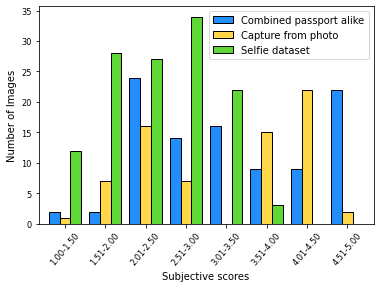
\includegraphics[width=0.65\textwidth]{figures/MobaiDS_Histogram.png}
    \caption{Histogram of MOS values calculated  for the images in each dataset. There is a clear difference between the quality of the Selfie dataset and the two others.}
    \label{fig:MobaiHistogram}
\end{figure}

Figure \ref{fig:MobaiDS} depicts three line plots of the standard deviation of the subjective scores on all images in each dataset. The plots show the subjective score distribution and they take into consideration the total standard deviation and the deviation of each participant group. Whenever the three lines have a low spread between each other it indicates that the deviation of the participant groups were similar. The lower the deviation the more the majority of the participants agreed upon a similar score. This was especially apparent in the Combined passport alike dataset (Figure \ref{fig:combinedpassportalikeSD}) which also generated the lowest total standard deviation of $\sigma = 0.6707$. The two remaining datasets (Figure \ref{fig:capturefromphotoSD} and \ref{fig:selfiedatasetSD}) received a similar total standard deviation of $\sigma = 0.7891$ and $\sigma = 0.7872$ respectively. Some images had greater variety than others. The Selfie dataset contained some of those, but all in all the general participants rated images alike. Even between the experts and non-experts, the evaluation was more or less equal. In fact non-experts had a slightly better standard deviation of $\sigma = 0.6908$, than the experts of $\sigma = 0.7608$ on the three datasets. 

Four images were chosen and previewed from each dataset. The first plot, Figure \ref{fig:combinedpassportalikeSD}, which showcases Combined passport alike, the first and second images would be considered excellent facial images. The experts rated these images very similarly which is apparent by the low deviation scores. The spread amongst non-experts were greater with deviations around 1.0. The two remaining images were of lower face quality, but the deviations were not affected by that.  


\begin{figure}[H]
 \centering 
    \subfloat
        {\hspace{1cm}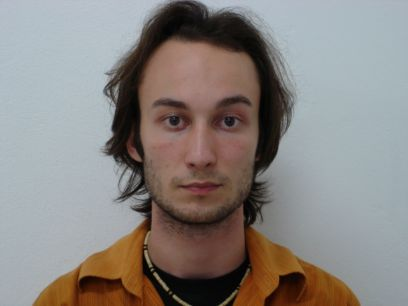
\includegraphics[scale = 0.1]{figures/042.jpg}\hspace{1.3cm}}
    \subfloat
        {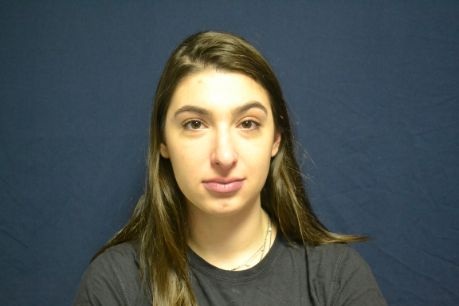
\includegraphics[scale = 0.1]{figures/132.jpg}\hspace{0.3cm}}
    \subfloat
        {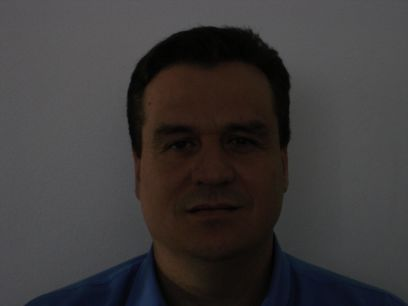
\includegraphics[scale = 0.1]{figures/145.jpg}\hspace{1.1cm}}
    \subfloat
        {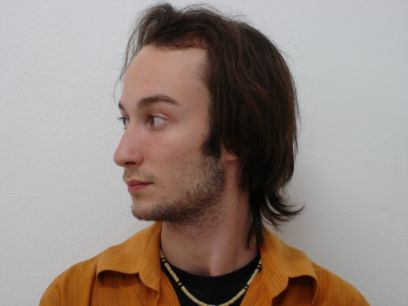
\includegraphics[scale = 0.1]{figures/234.jpg}\hspace{0.3cm}}
    \quad
    \addtocounter{subfigure}{-4}
    \subfloat[Combined passport alike dataset]
        {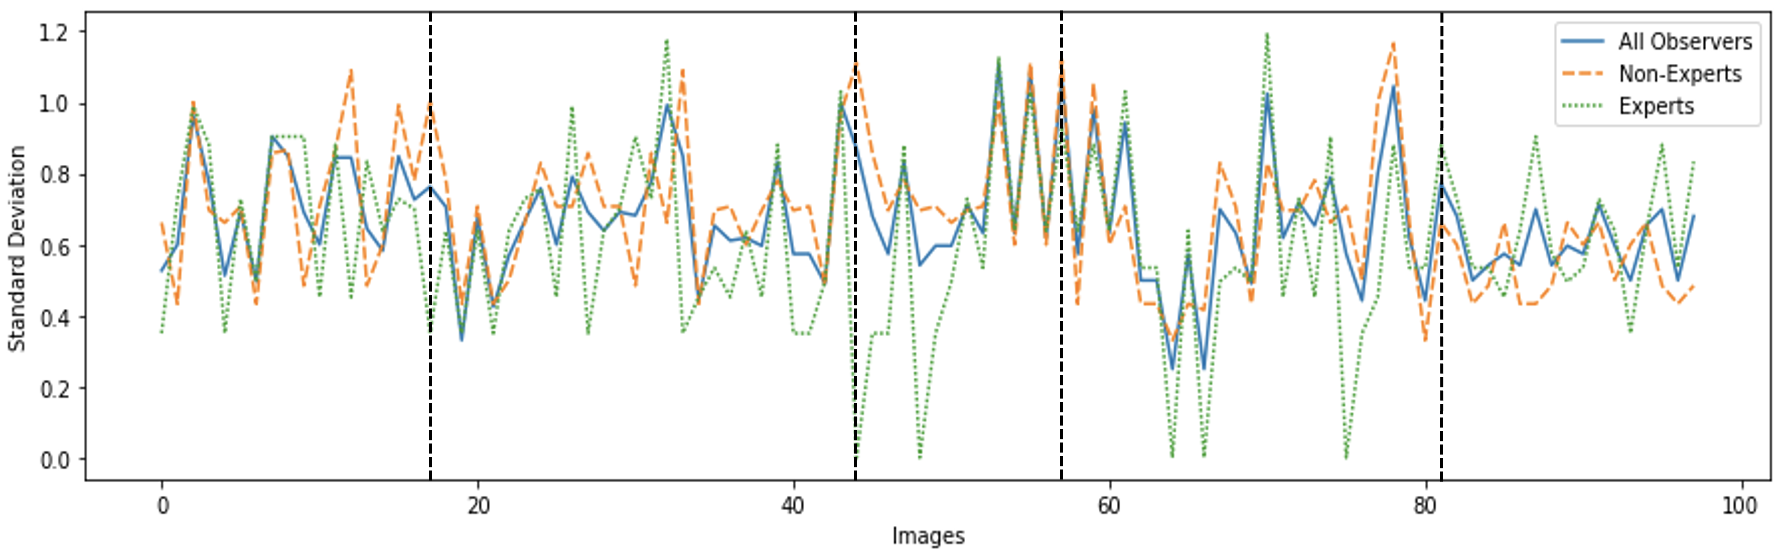
\includegraphics[width=1.0\textwidth]{figures/STD.png}\label{fig:combinedpassportalikeSD}}
        \quad
        \vspace{1cm}
    
    \subfloat
        {\hspace{0.7cm}
\includegraphics[scale = 0.12]{figures/004.jpg}\hspace{1.5cm}}
    \subfloat
        {
\includegraphics[scale = 0.12]{figures/101.jpg}\hspace{4.3cm}}
    \subfloat
        {
\includegraphics[scale = 0.12]{figures/198.jpg}\hspace{0.1cm}}
    \subfloat
        {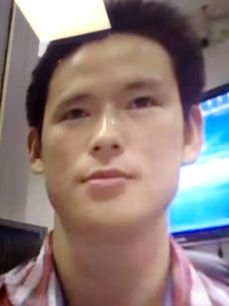
\includegraphics[scale = 0.12]{figures/204.jpg}\hspace{2.4cm}}
    \quad
    \addtocounter{subfigure}{-4}
    \subfloat[Capture from photo dataset]
         {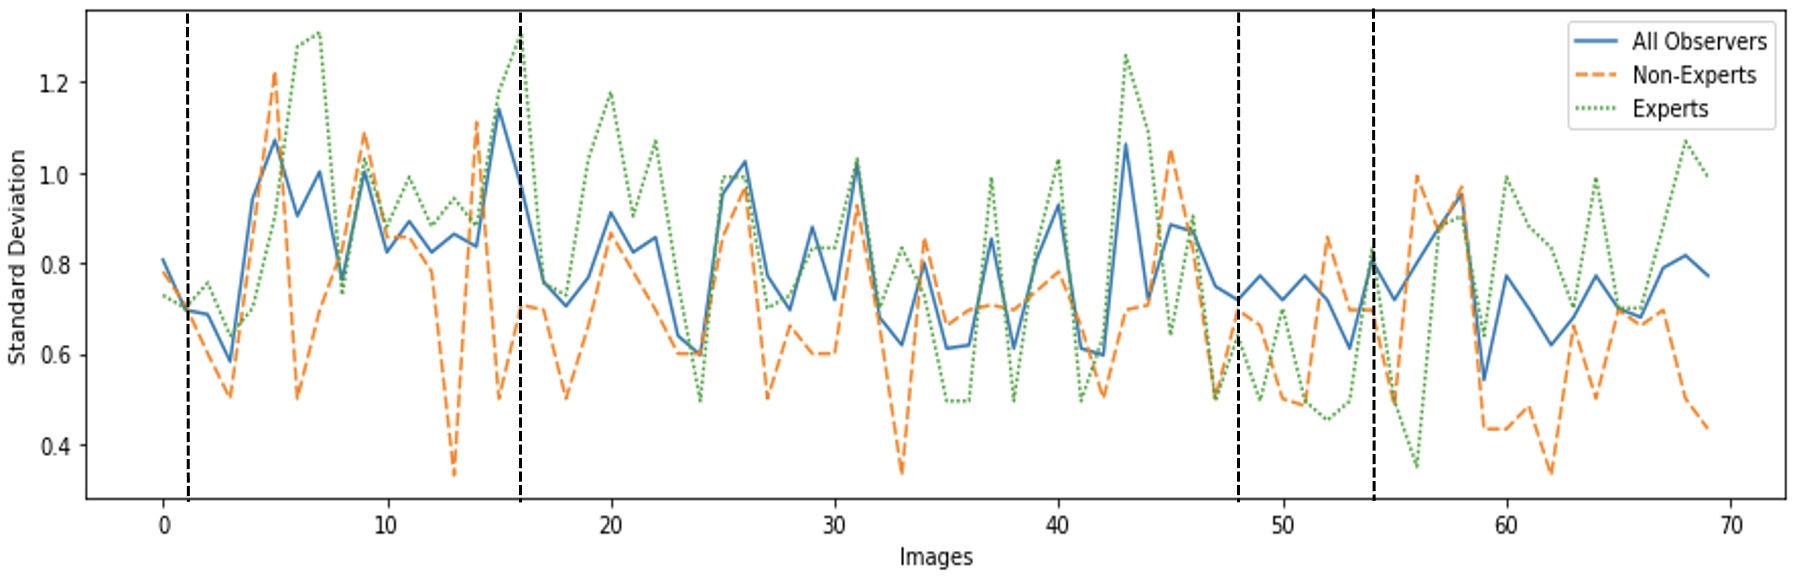
\includegraphics[width=1.0\textwidth]{figures/STD2.png}\label{fig:capturefromphotoSD}}
        \quad
        \vspace{1cm}
        
    \subfloat
        {\hspace{1.7cm}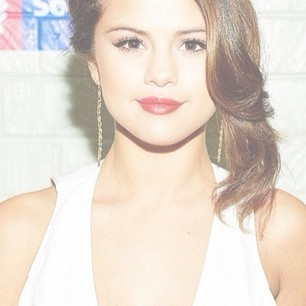
\includegraphics[scale = 0.1]{figures/086.jpg}\hspace{0.2cm}}
    \subfloat
        {
\includegraphics[scale = 0.1]{figures/098.jpg}\hspace{1.8cm}}
    \subfloat
        {
\includegraphics[scale = 0.1]{figures/187.jpg}\hspace{1.6cm}}
    \subfloat
        {\includegraphics[scale = 0.1]{figures/271.jpg}\hspace{1cm}}
    \quad
    \addtocounter{subfigure}{-4}
    \subfloat[Selfie dataset]
         {\includegraphics[width=1.0\textwidth]{figures/STD3.png}\label{fig:selfiedatasetSD}}
     \caption{Standard deviation values of the subjective scores given to each image in the three datasets. Sample images from each dataset are shown as examples.}
     \label{fig:MobaiDS}
\end{figure}

The four next facial images of Capture from photo in Figure \ref{fig:capturefromphotoSD} shows an overall equal standard deviation between the non-experts and experts. However, the second image had notable differences in the subjective scores between non-experts and experts. The standard deviation amongst experts were close to 1.2, which was the highest of the dataset. The great distribution of scores was likely due to the nature of the facial image. On one side the face is visible, but on the other side the image is taken from a computer screen which has heavily reduced the appearance of the face. This also applies to the last two images, however the standard deviation was lower and more even between the experts and non-experts.

The last four previewed facial images belong to the Selfie dataset (Figure \ref{fig:selfiedatasetSD}). The first image had an total deviation of 0.90. It was highly likely that the deviation of 0.90 was because the face was off-centered and not fully shown, which was the case for a large portion of the Selfie dataset images. However the second image had considerably lower standard deviation values. The face was barely visible which both participant groups assessed similarly. The scores of the experts on the last two images were more spread than the non-experts. 

\subsection{Evaluating the Performance of FIQMs}
The FIQMs presented in Chapter \ref{chap:FQA} use different approaches to predict the perceived face quality. Their predicted perception of quality is supposed to correlate with human assessment, which is the whole purpose of FIQMs. The objective predictions produced by the FIQMs were measured against human assessment to evaluate the accuracy of the proposed approaches. This evaluation was carried out by calculating the correlation coefficients. The sample Pearson correlation coefficient ($r$) was calculated as: 
\begin{equation}
    {\displaystyle r={\frac {\sum _{i=1}^{n}(x_{i}-{\bar {x}})(y_{i}-{\bar {y}})}{{\sqrt {\sum _{i=1}^{n}(x_{i}-{\bar {x}})^{2}}}{\sqrt {\sum _{i=1}^{n}(y_{i}-{\bar {y}})^{2}}}}}}
\end{equation}
where $n$ is the sample size, $x_{i}$ and $y_{i}$ denotes the individual sample scores from the objective and the subjective assessment respectively, while ${\bar {x}}={\frac {1}{n}}\sum _{i=1}^{n}x_{i}$ and ${\bar {y}}={\frac {1}{n}}\sum _{i=1}^{n}y_{i}$ represents the sample means from the objective and the subjective scores. Another type of correlation coefficient, the Spearman rank correlation coefficient ($\rho$) \cite{wiki:spearman} was also calculated because it does not assume that both variables are normally distributed.

The subjective scores were normalized in order to achieve the same ranking scale when being compared with the objective scores. Our subjective experiment initially had a categorical judgment with a scale from one to five, which was converted to scores between zero and one. It is easy to think that the MOS for each image should be divided by the number of score alternatives in the subjective experiment, which in this case was five. However it is worth noting that had we only divided the subjective scores by five, the lowest subjective scores achievable would be 0.2. This means that the FIQMs could provide scores from zero to one, while the subjective scores were from 0.2 to one. Dividing by five would therefore provide us with an uneven scoring scale where a score of five equals 100\% while the lowest score of one equals 20\% instead of 0\%. We needed a five-point scale that would increment the score alternatives with 25\% starting from 0\%. To properly convert a five-point scale to percentages we used the following equation (\ref{eqn:MOS}) on every image:

\begin{equation}
    MOS_{Normalized} = \frac{MOS - 1}{4}
    \label{eqn:MOS}
\end{equation}

\subsubsection{ISO Metrics}
\begin{figure}[h]
\centering
    \subfloat[Combined passport alike]
        {\includegraphics[scale = 0.31]{figures/ISO_Subjective1.png}\label{fig:iso_SUB1}}
    \subfloat[Capture from photo]
        {\includegraphics[scale = 0.31]{figures/ISO_Subjective2.png}\label{fig:iso_SUB2}}
    \subfloat[Selfie dataset]
        {\includegraphics[scale = 0.31]{figures/ISO_Subjective3.png}\label{fig:iso_SUB3}}
    \caption{2D scatter plots of the objective and subjective scores on the three datasets with objective scores along the x-axis and the subjective scores along the y-axis. The Spearman and Pearson correlation coefficients are shown above each plot.}
    \label{fig:corrISOsvsSub}
\end{figure}
\noindent 
As a first step in analyzing the performance of FIQMs, we calculate the correlation between the subjective scores and the objective scores calculated by the metrics. Figure \ref{fig:corrISOsvsSub} provides different plots of subjective against objective scores for the three introduced datasets. The correlation coefficients on Combined passport alike and Capture from photo were just shy of 0.5 which indicated a low to moderate association, whereas the correlation on the Selfie dataset was non-existent. The performance of ISO Metrics was clearly worse on the Selfie dataset relative to the two others. The FIQM was challenged by the dataset which was not surprising given that the images were of mediocre face quality which ISO Metrics often tends to over evaluate. In other words ISO Metrics was not suited for the Selfie dataset.  

\subsubsection{FaceQnet}
\begin{figure}[h]
\centering
    \subfloat[Combined passport alike]
        {\includegraphics[scale = 0.31]{figures/FaceQNet_Subjective1.png}\label{fig:face_SUB1}}
    \subfloat[Capture from photo]
        {\includegraphics[scale = 0.31]{figures/FaceQNet_Subjective2.png}\label{fig:face_SUB2}}
    \subfloat[Selfie dataset]
        {\includegraphics[scale = 0.31]{figures/FaceQNet_Subjective3.png}\label{fig:face_SUB3}}
    \caption{2D scatter plots of the objective and subjective scores on the three datasets with objective scores along the x-axis and the subjective scores along the y-axis. The Spearman and Pearson correlation coefficients are shown above each plot.}
    \label{fig:corrFACEQNETsvsSub}
\end{figure}
\noindent
The correlation between FaceQnet and the subjective scores regressed with each dataset the same way as ISO Metrics and the subjective scores did, shown in Figure \ref{fig:corrFACEQNETsvsSub}. The performance of the two FIQMs was comparable on all the datasets. Combined passport alike achieved the highest correlation of the datasets, with Spearman and Pearson values similar to the ones in Figure \ref{fig:iso_SUB1}. Like ISO Metrics, the performance of FaceQnet on Capture from photo was worse than Combined passport alike, but this time FaceQnet performed slightly worse than ISO Metrics. The performance on the Selfie dataset was even worse with a non-existing negligible correlation. A large part of the Selfie dataset images were rated zero. The facial images rated zero were mostly because the cropping part of FaceQnet failed. This happened when the cropping part failed to detect the face of the images. The images were therefore manually provided a score of zero. In other words, FaceQnet is not a suitable FIQM for the Selfie dataset. 

\subsubsection{Could We Use Different FIQMs Simultaneously?}
An interesting idea the team came up with, was if the correlation between the FIQMs and the subjective scores could be improved if a weighted average of the two FIQMs were used as the final FIQM. As a first step in such an approach, we simply gave the same weight to both FIQMs and tested the idea on the Combined passport alike and Capture from photo datasets. Since FaceQnet did not work for over 50\% of the images in the Selfie dataset, we found no reason to test this approach on that dataset. 

Figure \ref{fig:corrAVGvsSub} shows the correlation coefficients and the linear regression line calculated on the two datasets. The plot depicted in Figure \ref{fig:avg_SUB1} shows the highest correlation coefficients we ever achieved during our experiments. The $r$-value of 0.6045 and the $\rho$-value of 0.5942 were considerably higher than the correlation coefficients of the FIQMs individually. A value around 0.6 would indicate a moderate to strong correlation between the two data types. Even Capture from photo showed an increase in the correlation value. Initially, ISO Metrics performed better on the dataset than FaceQnet, but after the weighted average approach, the combined scores performed slightly better than ISO Metrics. Nevertheless, the correlation was still considered low to moderate. 
\begin{figure}[h]
\centering
    \subfloat[Combined passport alike]
        {\includegraphics[scale = 0.45]{figures/FIQMAVGSubjective1.png}\label{fig:avg_SUB1}}
    \subfloat[Capture from photo]
        {\includegraphics[scale = 0.45]{figures/FIQMAVGSubjective2.png}\label{fig:avg_SUB2}}
    \caption{2D scatter plots of the scores provided by using a weighted average of the FIQMs (with the same weight) on Combined passport alike and Capture from photo. The average FIQMs scores are displayed along the x-axis and subjective scores along the y-axis. The Spearman and Pearson correlation coefficients are presented above the plots.}
    \label{fig:corrAVGvsSub}
\end{figure}

\subsubsection{Error Method}
Plotting the results of the FIQMs against the subjective scores was not enough to assess the performance of the FIQMs on the datasets. Although the correlation coefficients on the datasets mostly were below 0.5 and indicated low to moderate correlation, error methods such as Root Mean Square Error (\acrshort{rmse}) can be used to track both the efficiency and accuracy of our FIQMs. The RMSE values were calculated by the following general formula: 
\begin{equation}
    RMSE = \sqrt{\frac{1}{N}\sum _{i=1}^{N}(Predicted_{i} - Actual_{i})^2}
    \label{eqn:RMSE}
\end{equation}
%
In Equation \ref{eqn:RMSE} $N$ corresponds to the number of samples, and in our case these were images. The predicted values denoted the objective scores by the FIQMs while the actual values were the corresponding subjective scores. This calculation gave us the standard deviation of the prediction errors. In other words, RMSE measured how far from the linear regression line the predicted values were. The closer to zero the scores were, the better the FIQMs predicted the right scores.

\begin{table}[h]
\caption{The calculated RMSE values of the FIQMs on the datasets relative to the subjective scores. The RMSE value was not calculated for the Selfie dataset with a weighted average of the FIQMs. The `X' symbolises this.}
\resizebox{\textwidth}{!}{%
\begin{tabular}{|
>{\columncolor[HTML]{EFEFEF}}c |
>{\columncolor[HTML]{FFFFFF}}c |
>{\columncolor[HTML]{FFFFFF}}c |
>{\columncolor[HTML]{FFFFFF}}c |}
\hline
\multicolumn{1}{|c|}{\cellcolor[HTML]{C0C0C0}\textbf{RMSE values}} &
  \multicolumn{1}{c|}{\cellcolor[HTML]{EFEFEF}ISO Metrics} &
  \cellcolor[HTML]{EFEFEF}FaceQnet &
  \multicolumn{1}{c|}{\cellcolor[HTML]{EFEFEF}FIQMs Weighted AVG} \\ \hline
Combined passport alike & 0.3675 & 0.3031 & 0.2262 \\ \hline
Capture from photo      & 0.3551 & 0.2887 & 0.2309 \\ \hline
Selfie dataset          & 0.4342 & 0.3253 & X \\ \hline
\end{tabular}%
}
\label{tab:RMSE}
\end{table}
%\noindent
The highest correlation coefficient, without using the weighted average approach on the FIQMs, was achieved on the Combined passport alike dataset with ISO Metrics as shown in Figure \ref{fig:iso_SUB1}. Although the correlation was around 0.5, the RMSE value was around 0.36, shown in Table \ref{tab:RMSE}. This meant that on average, the perceived quality predicted by ISO Metrics was off by $\pm$0.36 points compared to the actual subjective scores. Since our scale was from zero to one, 0.36 points off equaled an error of $\pm$36\% which was remarkably high. Even worse was the RMSE value on the Selfie dataset with ISO Metrics with a staggering error of 43\%. Despite having a lower correlation with the subjective scores on average, FaceQnet outperformed ISO Metrics on all datasets with its RMSE values. On average, FaceQnet´s errors were 0.8 points lower than ISO Metrics which equaled an error decrease of 20\%. 

The interesting results were those of the weighted average FIQMs. They ach-
ieved considerably better values than the FIQMs individually. Although an error of $\pm$0.22 and $\pm$0.23 in our case would be considered mediocre, the decrease could not be overlooked. Weighted average FIQMs had a decreased error rate of $\pm$0.14 points on Combined passport alike and $\pm$0.08, relative to ISO Metrics and FaceQnet. This equaled a decrease of 38.5\% and 25.4\% respectively. The accuracy of weighted average FIQMs was similar on the Capture from photo dataset. 

\subsection{Significance of Our Results}
Our results without any kind of validation were of little value. A validation had to be done in order to conclude whether our results were statistical significant. We had to be confident that our results could be replicated and that they did not occur by coincidence. 

The plots depicted in Figure \ref{fig:corrISOsvsSub} and Figure \ref{fig:corrFACEQNETsvsSub} showed for the most part, except for the Selfie dataset, a low to moderate correlation between the objective and subjective scores. The correlation coefficients were calculated with a 95\% confidence interval, which gave us a significance level of 0.05. The p-values of the correlation coefficients were calculated and the lower the p-value the more statistical significant our results were. Anything above a value of $p = 0.05$ was considered insignificant, because it meant that the likelihood of an uncorrelated system providing those exact coefficients randomly would be 5\%. 

Table \ref{tab:corrcoeff} show only the correlation coefficients that were considered statistically significant, i.e. we were 95\% confident the correlation coefficients did not occur by coincidence. The coefficients were replaced by an `X' symbol where the p-values were greater than the significance level and should therefore be taken with a grain of salt. All results regarding whether the FIQMs were correlated with the subjective scores on the Selfie dataset were confirmed to be uncorrelated with the high p-values. With a combination of high p-values and low correlation coefficients, it is highly likely that the objective and subjective scores were uncorrelated. The results gathered from the remaining datasets were within the significance level and were considered accurate.  


\begin{table}[h]
\caption{All correlation coefficients on the three datasets between ISO Metrics, FaceQnet, FIQMs Weighted AVG and the subjective scores. The `X'-symbol indicated the correlation coefficients that had a p-value higher than 0.05 and were therefore ignored. The coefficients were not calculated where the `-' symbol is placed.}
\resizebox{\textwidth}{!}{%
\begin{tabular}{l|
>{\columncolor[HTML]{FFFFFF}}c |
>{\columncolor[HTML]{FFFFFF}}c |
>{\columncolor[HTML]{FFFFFF}}c |
>{\columncolor[HTML]{FFFFFF}}c |
>{\columncolor[HTML]{FFFFFF}}c |
>{\columncolor[HTML]{FFFFFF}}c |}
\cline{2-7}
 &
  \multicolumn{2}{c|}{\cellcolor[HTML]{C0C0C0}\textbf{ISO Metrics}} &
  \multicolumn{2}{c|}{\cellcolor[HTML]{C0C0C0}\textbf{FaceQnet}} &
  \multicolumn{2}{c|}{\cellcolor[HTML]{C0C0C0}\textbf{FIQMs Weighted AVG}} \\ \cline{2-7} 
\textbf{} &
  Spearman $\rho$ &
  Pearson $r$ &
  Spearman $\rho$ &
  Pearson $r$ &
  Spearman $\rho$ &
  Person $r$ \\ \hline
\multicolumn{1}{|l|}{\cellcolor[HTML]{C0C0C0}Combined passport alike} &
  0.4425 &
  0.4721 &
  0.4885 &
  0.4525 &
  0.5942 &
  0.6045 \\ \hline
\multicolumn{1}{|l|}{\cellcolor[HTML]{C0C0C0}Capture from photo} &
  0.3704 &
  0.4330 &
  X &
  0.2843 &
  0.4398 &
  0.4550 \\ \hline
\multicolumn{1}{|l|}{\cellcolor[HTML]{C0C0C0}Selfie dataset} &
  X &
  X &
  X &
  X &
  - &
  - \\ \hline
\end{tabular}%
}
\label{tab:corrcoeff}
\end{table}
%\noindent


\section{Second Experiment}
\label{sec:secondExperiment}
This section is about the second experiment we conducted based on our own NFC dataset of 450 images, and the results we achieved. A key goal the team considered was having the NFC dataset consist of varying face quality to achieve a balanced dataset. A histogram of the MOS values calculated in the second subjective experiment on the NFC dataset is depicted in Figure \ref{fig:NFCHistogram}. One can see how the different quality categories are represented to an acceptable level. Images of specific quality were not over represented relative to the other quality categories and there exist a nice distribution in the dataset with images of varying quality which was the goal of the group. 

\begin{figure}[h]
    \centering
    \includegraphics[width=0.5\textwidth]{figures/NFC_Histogram.png}
    \caption{Histogram of the subjective scores on the NFC dataset.}
    \label{fig:NFCHistogram}
\end{figure}

\subsection{Results of the Subjective Evaluation}
The MOS of each image was calculated as we did in the first subjective experiment in Section \ref{sec:SubAssessment}. The subjective scores of the NFC dataset provided by the participants correlated closely. The average standard deviation of the subjective scores was calculated to be $\overline{\sigma} = 0.53$ which was substantially lower than those of the datasets in the first subjective experiment mentioned in Section \ref{sec:SubAssessment}. This time the experiment was not split into several sessions to prevent fatigue even though it consisted of several times the facial images of the first subjective experiment. With that in mind the average standard deviation was lower, which goes to show how the subjective experiment aspects mentioned in Section \ref{sec:SubjectiveAspects} mattered to a lesser degree since we were collecting ground truth data. Provided that six subjects participated in the subjective experiment and only two of those were experts we found no reason to compare the standard deviations between those types of participants.


\subsection{Results of the Objective Evaluation}
An important metric we voluntary wanted to measure was how the FIQMs performed on distorted images relative to their corresponding undistorted ones. This was tested on a subset of the NFC dataset which consisted of the 200 distorted images and their 50 corresponding original images. In order to assess how the FIQMs performed we first had to analyze how the subjective scores were distributed. A histogram of the MOS values for different types of distortions are shown in Figure \ref{fig:NFC2HistogramSUB}. From Figure \ref{fig:NFC2HistogramSUB} it is clear that the distortions we added to the images did not have a considerable affect on the subjective scores. It is interesting to investigate how such distortions can affect the performance of FIQMs.

\begin{figure}[h]
    \centering
    \includegraphics[width=0.5\textwidth]{figures/NFC_HistogramSUB.png}
    \caption{Histogram of the subjective scores of the original images and their corresponding distorted images in the NFC dataset.}
    \label{fig:NFC2HistogramSUB}
\end{figure}

\begin{figure}[h]
\centering
    \subfloat[ISO Metrics scores]
        {\includegraphics[ width=0.47\textwidth]{figures/NFC_HistogramISO.png}\label{fig:HistogramISO}}
    \subfloat[FaceQnet scores]
        {\includegraphics[width=0.47\textwidth]{figures/NFC_HistogramFaceQnet.png}\label{fig:HistogramFACE}}
    \caption{Histogram of the objective scores of the original images and their corresponding distorted images in the NFC dataset.}
    \label{fig:NFC2Histogram}
\end{figure}

Figure \ref{fig:NFC2Histogram} showcases how the FIQMs performed on the original and distorted images. Even though the scores provided vastly differed from the subjective scores, one can see how the objective scores highly correlated between the different distortions. Among the FIQMs, FaceQnet had an overall better performance on the types of distortions we added relative to ISO Metrics. Its scores correlated close to perfect which is shown in Figure \ref{fig:NFCFaceCorr}. Three out of four distortions had correlation coefficients above 0.8, which is considered a very strong positive correlation. Only the Telegram compression on FaceQnet performed slightly worse with a moderate to high correlation. ISO Metrics performed likewise, however the scores were more spread as shown in Figure \ref{fig:HistogramISO}. The scores of facial images with noise differed noticeably from its original ones. Facial images with noise also had a significantly lower correlation than the other distortions, shown in Figure \ref{fig:NFCISOCorr}. The FIQM struggled with facial images with noise which is clear by the moderate correlation coefficients close to 0.5, relative to the other distortions which are considered strongly correlated. Not only did the correlation coefficients confirm that FaceQnet performed better on the distortions, but the FIQM had considerably lower RMSE values on $\frac{3}{4}$ distortions than ISO Metrics. Only by looking at the RMSE values mentioned above each plot depicted in Figure \ref{fig:NFCFaceCorr} and Figure \ref{fig:NFCISOCorr}, it is clear that ISO Metrics is less consistent than FaceQnet when assessing distorted images. 

\begin{figure}[H]
\centering
    \subfloat
        {\includegraphics[width=0.37\textwidth]{figures/FaceQnetBlur.png}}
    \subfloat
        {\includegraphics[width=0.37\textwidth]{figures/FaceQnetNoise.png}}
        \quad
    \subfloat
        {\includegraphics[width=0.37\textwidth]{figures/FaceQnetPhotoshop.png}}
    \subfloat
        {\includegraphics[width=0.37\textwidth]{figures/FaceQnetTelegram.png}}
    \caption{2D scatter plots of FaceQnet scores on the original images along the x-axis and the distorted images along the y-axis. All correlation coefficients are given with a 95\% confidence interval. RMSE values are included above the plots.}
    \label{fig:NFCFaceCorr}
\end{figure}

\begin{figure}[h]
\centering
    \subfloat
        {\includegraphics[width=0.365\textwidth]{figures/ISOBlur.png}}
    \subfloat
        {\includegraphics[width=0.365\textwidth]{figures/ISONoise.png}}
        \quad
    \subfloat
        {\includegraphics[ width=0.365\textwidth]{figures/ISOPhotoshop.png}}
    \subfloat
        {\includegraphics[width=0.365\textwidth]{figures/ISOTelegram.png}}
    \caption{2D scatter plots of ISO Metrics scores on the original images along the x-axis and the distorted images along the y-axis. All correlation coefficients are given with a 95\% confidence interval. RMSE values are included above the plots.}
    \label{fig:NFCISOCorr}
\end{figure}

\subsection{Evaluating the Performance of FIQMs}
The correlation between the FIQMs and the collected subjective scores was calculated and plotted in Figure \ref{fig:ourDS1corr}. A 0.05 significance level was used when calculating the correlation coefficients. The coefficients ranged between 0.32 to 0.42 which meant there was a weak association between the objective and subjective scores. Using a weighted average of the two FIQMs did not show a significant difference. There were no clear difference between the performance of either FIQM on our dataset. Even though the correlation was weak, the result were not entirely negative. Our dataset was supposed to challenge the FIQMs by introducing new measures they had not been exposed to or created to assess, which was the case. 

\begin{figure}[H]
\centering
    \subfloat[ISO Metrics]
        {\includegraphics[scale = 0.31]{figures/NFCISOSUB.png}\label{fig:our1_ISO}}
    \subfloat[FaceQnet]
        {\includegraphics[scale = 0.31]{figures/NFCFACESUB.png}\label{fig:our1_FACE}}
    \subfloat[FIQMs Weighted AVG]
        {\includegraphics[scale = 0.31]{figures/NFCWeightedAVG.png}\label{fig:our1_AVG}}
    \caption{2D scatter plots of the scores on the NFC dataset with objective scores along the x-axis and subjective scores along the y-axis. The Spearman and Pearson correlation coefficients are shown above the plots.}
    \label{fig:ourDS1corr}
\end{figure}

\subsubsection{Score Distribution on Distorted Images} 

The spider chart in Figure \ref{fig:spiderMask} takes a closer look into how the FIQMs reacted to the different face mask usages. The subjective scores for 0940.jpg and 1133.jpg were lower than the two other face mask images because the face is more covered and therefore less visible. ISO Metrics did not react to that whatsoever, but Face-Qnet did provide slightly lower scores, but the change was very minor. Regarding the spider plot of the oblique angled images depicted in Figure \ref{fig:spiderTilted}, both FIQMs provided lower scores than the subjective, but the ISO Metrics scores were consistent where as FaceQnet had larger differences between the facial images.

The two spider plots depicted in Figure \ref{fig:SpiderDist1} and Figure \ref{fig:spiderDist2} are used to show the score distribution of the previewed distorted facial images. On image 0329.jpg in Figure \ref{fig:SpiderDist1} we can see how ISO Metrics predicted equal scores, but the facial image with noise had a major effect on the score. This is consistent with the histogram in Figure \ref{fig:HistogramISO}. Even the Photoshop compression received double the score of its original image. FaceQnet had an overall more consistent quality perception close to the subjective scores. Image 0718.jpg in Figure \ref{fig:spiderDist2} again showed how FaceQnet was not affected by adding any of our distortions. The plot reinforces the claim that the distribution of objective scores on distorted images were negligible with FaceQnet, which is shown in Figure \ref{fig:HistogramFACE}. The FaceQnet scores were quality wise closely related to the subjective scores, whereas the quality perception by ISO Metrics was off. This time, the FIQM gave much more consistent scores with no large spikes, which goes to show its inconsistency.


\begin{figure}[H]
\centering
    \subfloat[Different use of face masks.]
        {\includegraphics[width=0.42\textwidth]{figures/SpiderMask.png}} \\
    \subfloat[0926.jpg]
        {\includegraphics[scale = 0.09]{figures/926.png}\hspace{0.4cm}}
    \subfloat[0940.jpg]
        {\includegraphics[scale = 0.09]{figures/940.png}\hspace{0.4cm}}
    \subfloat[1133.jpg]
        {\includegraphics[scale = 0.09]{figures/1133.png}\hspace{0.4cm}}
    \subfloat[1152.jpg]
        {\includegraphics[scale = 0.09]{figures/1152.png}\hspace{0.4cm}}
    \caption{Spider chart of the objective and subjective scores on different face mask images.}
    \label{fig:spiderMask}
\end{figure}
\newpage

\begin{figure}[H]
\centering
    \subfloat[Different oblique angles.]
        {\includegraphics[width=0.4\textwidth]{figures/SpiderTilted.png}} \\
    \subfloat[0035.jpg]
        {\includegraphics[scale = 0.12]{figures/0035.jpg}\hspace{0.4cm}}
    \subfloat[0143.jpg]
        {\includegraphics[scale = 0.12]{figures/0143.jpg}\hspace{0.4cm}}
    \subfloat[0151.jpg]
        {\includegraphics[scale = 0.12]{figures/0151.jpg}\hspace{0.4cm}}
    \subfloat[0151.jpg]
        {\includegraphics[scale = 0.12]{figures/0172.jpg}\hspace{0.4cm}}
    \subfloat[0246.jpg]
        {\includegraphics[scale = 0.12]{figures/0246.jpg}\hspace{0.4cm}}
    \caption{Spider chart of the objective and subjective scores on images with different oblique angles.}
    \label{fig:spiderTilted}
\end{figure}

\raggedbottom

\begin{figure}[H]
    \centering
    \subfloat[0329.jpg distorted.]
        {\includegraphics[width=0.4\textwidth]{figures/SpiderDistortions.png}} \\
    \subfloat[Original.]
        {\includegraphics[scale = 0.09]{figures/0329.jpg}\hspace{0.7cm}}
    \subfloat[Blur.]
        {\includegraphics[scale = 0.09]{figures/0329blur.jpg}\hspace{0.7cm}}
    \subfloat[Noise.]
        {\includegraphics[scale = 0.09]{figures/0329noise.jpg}\hspace{0.7cm}}
    \subfloat[Photoshop\\ compression.]
        {\includegraphics[scale = 0.09]{figures/0329photoshop_compression.jpg}\hspace{0.7cm}}
    \subfloat[Telegram\\ compression.]
        {\includegraphics[scale = 0.09]{figures/0329telegram_compression.png}\hspace{0.7cm}}
    \caption{Spider chart of the objective and subjective scores on original and distorted facial images.}
    \label{fig:SpiderDist1}
\end{figure}

\newpage

\begin{figure}[H]
\centering
    \subfloat[0718.jpg distorted.]
        {\includegraphics[width=0.42\textwidth]{figures/SpiderDistortions2.png}
        \label{fig:dist2}} \\
     \subfloat[Original.]
        {\includegraphics[scale = 0.09]{figures/0718.jpg}\hspace{0.7cm}}
    \subfloat[Blur.]
        {\includegraphics[scale = 0.09]{figures/0718blur.jpg}\hspace{0.7cm}}
    \subfloat[Noise.]
        {\includegraphics[scale = 0.09]{figures/0718noise.jpg}\hspace{0.7cm}}
    \subfloat[Photoshop\\ compression.]
        {\includegraphics[scale = 0.09]{figures/0718photoshop_compression.jpg}\hspace{0.7cm}}
    \subfloat[Telegram\\ compression.]
        {\includegraphics[scale = 0.09]{figures/0718.jpg}\hspace{0.7cm}}
    \caption{Spider chart of the objective and subjective scores on original and distorted facial images.}
    \label{fig:spiderDist2}
\end{figure}
\chapter{Conclusion}
\label{chap:Conclusion}
 Now that we have looked at the various aspects that went into the development of the web application and the subjective experiment, it is time to reflect on the journey our group has gone through the last months. In Section \ref{sec:objective} we discuss how the application turned out and how the user test supported that the requirements were fulfilled. Further in Section \ref{sec:subjectiveevaluation}, we reflect upon our subjective experiments. In Section \ref{sec:resultsevaluation} we summarize our results. To end the chapter, we evaluate the group work (Section \ref{sec:groupworkevaluation}), learning outcome (Section \ref{sec:learningoutcome}) and introduce future work (Section \ref{sec:futurework}).

\section{Objective Assessment Evaluation}
\label{sec:objective}
To evaluate our work done in the objective assessment, we have looked at how well we managed to complete the task Mobai gave us. Based on the requirements stated in Section \ref{sec:requirements} and the use cases showcased in Figure \ref{fig:UseCase}, we can see that we have managed to build and complete all the main functionality and requirements that Mobai had given us in the objective assessment. Given the feedback from the user testing showcased in Table \ref{table:usertesttasks}, all functionality worked and was set to ``Satisfactory'' by the Product Owner. From the user testing questions in Table \ref{table:usertestquestions}, we got some feedback regarding doing some minor design changes to the frontend. Overall we have done what Mobai asked us and according to their feedback, they were satisfied. 

\section{Subjective Experiment Evaluation}
\label{sec:subjectiveevaluation}
As introduced in Section \ref{sec:SubjectiveAspects}, there were several aspects to take into account when conducting a subjective experiment. We spent much time in researching and analyzing different aspects and platforms when deciding the structure of the experiment. Collecting observers was more difficult with the ongoing COVID-19 restrictions. Ideally we wanted to invite observers to perform the subjective experiment in a controlled environment which was not possible. However, conducting a subjective experiment on the web ended up being surprisingly less complicated than we thought. 

\section{Evaluation of the Results}
\label{sec:resultsevaluation}
When it comes to the two FIQMs, we can conclude that they had a non-existent correlation between each other on Combined passport alike and the Selfie dataset, and a positive weak correlation on Capture from photo, as shown by the scatter plot depicted in Figure \ref{fig:corrFIQMs}. However, on the same datasets, the correlations were remarkably higher when comparing the objective scores to the subjective scores. Both ISO Metrics and FaceQnet performed similar as well on the Combined passport alike dataset with a moderate correlation shy of 0.5, as shown in Figure \ref{fig:corrISOsvsSub} and Figure \ref{fig:corrFACEQNETsvsSub}. On the Capture from photo dataset, ISO Metrics outperformed FaceQnet by having a moderate correlation, while FaceQnet´s correlation coefficients were considered weak. The dataset in which the FIQMs performed crucially poor, were the Selfie dataset. Both FIQMs had a non-existent association with the ground truth data. With regards to FaceQnet, the FIQM did not work for that particular dataset, because the faces in the images were not detected and therefore the cropping phase became defective. ISO Metrics on the other hand, struggled with estimating the correct quality because the facial images of the Selfie dataset greatly differed in quality relative to the two other datasets. The facial images were either off-centered, too zoomed in or a combination of both, which ISO Metrics did not react accordingly to. The strongest association achieved was done by combining the scores from ISO Metrics and FaceQnet on Combined passport alike. With Pearson and Spearman values around 0.6, we can conclude that combining the FIQMs can be a reliable choice for datasets where the facial images checks several of the bullet points in what defines a good facial image listed in Section \ref{item:passport}.

The performance of the FIQMs with regards to face masks were subpar. The perceived quality by ISO Metrics did not change with different face masks coverings, whereas FaceQnet had very minor differences. The two FIQMs can not be considered reliable when assessing face masks. The same can not be said for oblique angled facial images. The FIQMs showed minor differences when assessing those types of facial images. 

Assessing the quality of distorted facial images did affect the perceived quality for ISO Metrics, but not for FaceQnet. The last mentioned FIQM perceived the quality consistently with close to perfect association with the original images shown in Figure \ref{fig:kernelFACE} and Figure \ref{fig:SpiderDistortions}. The FIQM should be considered accurate when predicting the perceived quality on the distortions we added, which was not entirely the case for ISO Metrics. The FIQM had trouble assessing facial images with noise and was less accurate than FaceQnet when assessing blur and compression done in Photoshop shown in Figure \ref{fig:kernelISO}. 

\section{Group Work Evaluation}
\label{sec:groupworkevaluation}
Although only working from home and communicating on digital platforms, the collaboration between the group members has been great. We have worked mostly together and all agreements and deadlines were met. The workflow throughout the project was consistent which ended up in great quality work. Toggl, as mentioned in the project plan, was a great tool for following each members working tasks. The group members have helped each other with reviewing their work. The thesis writing started early and we are satisfied with the outcome. 

\section{Learning Outcome}
\label{sec:learningoutcome}
By working closely together the past months, we have learned the importance of having a strict schedule and expectations among the members to ensure everyone keep their morale and the good work throughout the project. We experienced that not having clear deadlines resulted in incompletion of working tasks. These types of lacks required more time spending on reviewing the code and report. On the programming side, the group has learned new programming languages, tools, libraries and how these interact. We may not have come up with the best approach, however the requirements were met and the web application is working. No one in the team had developed a web application before, resulting in a new experience for all members. Coding wise, it was manageable to create the backend in Python and a frontend UI in React.js. However, no one had experience in making them interact with each other, so the APIs could be developed in a more well-designed way. In terms of research, the members have developed new abilities throughout the project by retrieving information and using it in our work. This project has also helped us getting better to write English and presenting our work in a more scientific way. We have learned the importance of how to conduct subjective experiments. With this foundation and all the supplied aspects to bare in mind, we can now create comprehensive subjective experiments to collect subjective scores. 

\section{Future Work}
\label{sec:futurework}
We managed to include everything specified in Chapter \ref{chap:objective}. Since one of the requirements was to easy facilitate new FIQMs to be added into the web application, using the application in further work was a reality. Mobai has stated that this application will be a part of their face recognition system, where the web application works as a sieve to filter out low-quality images. Chapter \ref{chap:objective} can be used as documentation to describe the different technologies used to develop the web application.

The two FIQMs utilized in this project, can be studied further. Whereas both provide quality scores to facial images, they act differently. To give a better evaluation of facial images, studying the weighted average between the two FIQMs can provide improved accuracy of the quality scores. 

Our dataset, described in Section \ref{sec:ownData}, was outperforming the datasets provided by Mobai. It consisted of more facial images, distortions and new aspects. The new aspects consisting of camera angels and wearing face masks tested the FIQMs in a new way. Mobai is able to use the NFC dataset in their further work of testing new FIQMs and face recognition systems. 


\chapter*{\bibname}
\printbibliography[heading=none]


\appendix
%\chapter{Project Plan}
\label{app:project-plan}

\cleardoublepage

\includepdf[pages=-]{appendices/a-projectPlan/Prosjektplan.pdf}


%\chapter{Project Assignment}
\label{app:project-assignment}

\cleardoublepage
\includepdf[pages=-]{appendices/b-assignment/OppgaveBeskrivelse.pdf}
%\chapter{Project agreements}

\cleardoublepage
\includepdf[pages=-]{appendices/c-agreements/NTNUAgreement}
\cleardoublepage
\includepdf[pages=-]{appendices/c-agreements/MobaiAgreement}
%\chapter{Results}
\label{app:results}

\includepdf[pages=-]{appendices/d-results/Combined_passport_alike_scores.pdf}
\includepdf[pages=-]{appendices/d-results/Capture_from_photo_scores.pdf}
\includepdf[pages=-]{appendices/d-results/Selfie_dataset_scores.pdf}
%\chapter{Meeting reports}

% TODO: add table of contents for meeting reports?

%\dominitoc% Initialization
%\tableofcontents
\chapter{Meetings With Project Supervisor}
\label{appendix:supervisor}

We had regular meetings with our project supervisor Ali on Mondays at 12:00. There were also some extraordinary meetings during the project.

% TODO: add the latest meeting reports, after the 10th of May.

\section*{Meeting with project supervisor 11.01.2021}
\subsection*{Planned agenda}
\begin{itemize}
    \item Getting started.
\end{itemize}

\subsection*{Summaries}
\begin{itemize}
    \item Think about how we will run the user tests?
    \item Where will we get face images? From Mobai?
    \item About the project report: potential for a publication?
\end{itemize}

\subsection*{Agenda for the next week}
\begin{itemize}
    \item Prepare a time plan.
    \item Should we write everything in English?
\end{itemize}



\section*{Meeting with project supervisor 18.01.2021}
\subsection*{Planned agenda}
\begin{itemize}
    \item Explain the project further to the supervisor.
    \item Show the time plan to the supervisor.
        \begin{itemize}
            \item The subjective experiment will take more than a month. Probably one and a half months.
    \end{itemize}
    \item Discuss further work
    \begin{itemize}
        \item The final product: local application or web application?
        \item Time requirements for the subjective assessment (manual observations). How long will it take? Probably many weeks.
    \end{itemize}
    \item Show and discuss the group rules.
\end{itemize}

\subsection*{Summaries}
\begin{itemize}
    \item How should we conduct the subjective experiment?
    \begin{itemize}
        \item Evaluate which platform we want to use and why we decide to use it. We can use QuickEval, SurveyMonkey, LimeSurvey, or some other platform.
        \item The images should be shown in a random order.
        \item What can we include in our dataset/subjective experiments that are unique?
    \end{itemize}
    \item Create a structure of the thesis, with names of the chapters and sections. Include the number of pages. 
\end{itemize}

\subsection*{Agenda for the next week}
\begin{itemize}
    \item Send research papers and group rules to Ali.
    \item Write the first draft for the structure of the thesis. Write down the chapter names and number of pages.
\end{itemize}



\section*{Meeting with project supervisor 27.01.2021}
\subsection*{Planned agenda}
\begin{itemize}
\item Show our project plan
\item Show our draft of the project structure with chapter headings and number of pages.
\item Subjective assessment: 
    \begin{itemize}
    \item Which score range is the best one to use? 1-5, 1-20?
    \item How should we do the survey? Score one and one image? Put multiple images in order of quality score?
    \end{itemize}
\item In the report, can we use different tenses (past, present, future) in the same paragraph?
\end{itemize}

\subsection*{Summaries}
\begin{itemize}
    \item Draft of the project structure:
    \begin{itemize}
        \item Add numbers to the chapters.
        \item Add the number of pages (and required time) to sections.
        \item The sections we have written down look good.
        \item Maybe move the subjective assessment to a separate chapter (if it’s long and makes sense to put it in a separate section). 
        \item Excessive theory that is not used in the report will affect the grading of the report.
    \end{itemize}
    \item Creating the subjective assessment:
    \begin{itemize}
        \item Check a few datasets that are out there, see what they do and how they do it.
        \item Display the images in random order.
    \end{itemize}
    \item About the thesis writing.
    \begin{itemize}
        \item Don’t jump between tenses. Use Past tense.
        \item In the results, use past or present tense.
        \item Do a shift to present in the end.
        \end{itemize}
\end{itemize}

\subsection*{Agenda for the next week}
\begin{itemize}
    \item Send the project plan to Ali.
    \item Look into one or two data sets.
    \item Finalize our time plan.
\end{itemize}



\section*{Meeting with project supervisor 01.02.2021}
\subsection*{Planned agenda}
\begin{itemize}
    \item Go through our project plan and the comments from Ali.
    \item Show the supplementary agreement from Mobai. Any thoughts?
    \item What is a data set? A collection of images?
    \item Our goal with the application. How should it work?
\end{itemize}

\subsection*{Summaries}
\begin{itemize}
    \item We went through the project plan and wrote down the comments from Ali.
    \item Speak to Tom about the supplementary agreement.
    \item Speak with Mobai about how the application should work. 
    \item Dataset:
    \begin{itemize}
        \item It’s called a dataset or datasets (one word). \item Dataset: a collection of images.
        \item We evaluate the quality of an image.
        \item The quality of the dataset: how we present and run the test decides the quality of the dataset. The higher the quality, the more reliability.
    \end{itemize}
\end{itemize}

\subsection*{Agenda for the next week}
\begin{itemize}
    \item Create a pilot test for the subjective experiment. Be prepared for comments and changes. Have a finished test by the 15th of February.
\end{itemize}



\section*{Meeting with project supervisor 08.02.2021}
\subsection*{Planned agenda}
\begin{itemize}
    \item Show our pilot of the subjective experiment.
    \item Mobai’s and Ali’s definition of a quality image are two different things? 
    \item We will use SurveyMonkey/QuickEval for the subjective experiment, with random image order. 
    \item Our dataset consists of 280 images. Mobai wants all participants in the subjective experiment to rate all of the 280 images in the dataset.
    \item How do we perform the subjective experiment?
    \item How do we pick the best 100 images from the “Faces in the wild” dataset?
    \item Invite Ali to join a meeting with Mobai.
\end{itemize}

\subsection*{Summaries}
\begin{itemize}
    \item Use the same rating system for the experiment.
    \item Can we split the images in the subjective experiment into three sets? Ask Mobai.
    \item How do we perform the subjective experiment?
    \begin{itemize}
        \item Suggestion for the subjective experiment: split the experiment into 3 sessions. One session for each image folder in the dataset. Should the sessions be split over multiple days or the same day with breaks between sessions?
        \item Remember: if we split into multiple sessions we need to track the sessions of the participants so we can connect the different sessions to the same participant.
        \item Have a training set first to train the participants for the experiment?
        \item Don’t mention “quality” (or, define clearly what we mean by quality.
        \item We want to test the face recognition quality.
        \item Define who we want to ask to take the subjective experiment.
    \end{itemize}
    \item How do we pick the best 100 images from the “Faces in the wild” dataset?
    \begin{itemize}
        \item Variant image quality matters. I.e., pick a variety of images where the faces are covered or less visible in some way, e.g. with sunglasses, different poses, different perspectives and so on.
        \item Also pick images where the faces are clearly visible (“passport-like”).
    \end{itemize}
    \item There are three kinds of metrics:
    \begin{itemize}
        \item Full access metrics
        \item Reduced reference
        \item No reference
    \end{itemize}
    \item Ali will join our next meeting with Mobai on Tuesday.
\end{itemize}

\subsection*{Agenda for the next week}
\begin{itemize}
    \item Create clear instructions for the users of the subjective experiment. What do we want the users to evaluate? 
    \item Test the datasets with the IQMs and check out the results.
\end{itemize}



\section*{Meeting with project supervisor 11.02.2021}
\subsection*{Planned agenda}
\begin{itemize}
    \item Talk about our meeting with Mobai on Tuesday.
    \item Use face image quality score from 1-10?
\end{itemize}

\subsection*{Summaries}
\begin{itemize}
    \item Find the smallest of all of the images in the datasets. Downsize all the images to the same size (and keep the aspect ratio).
    \item Use the  face image quality scores 1-5, or maybe 1-7?
\end{itemize}



\section*{Meeting with project supervisor 15.02.2021}
\subsection*{Planned agenda}
\begin{itemize}
    \item Go through the comments on the survey instructions
    \item Should all of the images be of the same size?
    \item Dataset 3, “Faces in the wild” is not good enough.
\end{itemize}

\subsection*{Summaries}
\begin{itemize}
    \item We went through the survey instructions and made the necessary adjustments:
    \begin{itemize}
        \item We can create a control dataset. We can use images of ourselves.
        \item We will create image lineups from the control dataset.
        \item Have Mobai rate the images in the survey instruction.
    \end{itemize}
\end{itemize}



\section*{Meeting with project supervisor 22.02.2021}
\subsection*{Planned agenda}
\begin{itemize}
    \item Update on our current status:
    \begin{itemize}
        \item Currently working on the frontend and backend for the web application.
    \end{itemize}
\end{itemize}

\subsection*{Summaries}
\begin{itemize}
    \item We will continue working on the web application.
\end{itemize}



\section*{Meeting with project supervisor 01.03.2021}
\subsection*{Planned agenda}
\begin{itemize}
    \item Show experiment instructions:
    \begin{itemize}
        \item At the beginning of the instructions, include “a very brief intro about the face recognition system”?
        \item Delete the slides at the end?
    \end{itemize}
\end{itemize}

\subsection*{Summaries}
\begin{itemize}
    \item Survey instructions:
    \begin{itemize}
        \item Send 15 images each to Mobai and have them rate all of them. Ask Guoqiang to have them rated by Wednesday.
        \item In the image lineups: image with the lowest score on the left.
        \item Random is good. In a lineup, we include different pictures of each of the members. Have a 1-5 rating for each member.
    \end{itemize}
    \item Write about our dataset in the thesis.
    \item Before sending out the subjective experiment:
    \begin{itemize}
        \item Test the experiment ourselves first.
        \item Get approval of the experiment by sending it to Ali and Guoqiang.
        \item Then send it out to a few people, not all of them.
    \end{itemize}
    \item Start writing about things in the thesis that will not change.
\end{itemize}

\subsection*{Agenda for the next week}
\begin{itemize}
    \item Send 15 images each to Mobai and have them rate all of them. Ask Guoqiang to have them rated by Wednesday.
    \item Ask mobai if they want us to create our own dataset.
\end{itemize}



\section*{Meeting with project supervisor 08.03.2021}
\subsection*{Planned agenda}
\begin{itemize}
    \item About the subjective experiment on QuickEval.
\end{itemize}

\subsection*{Summaries}
\begin{itemize}
    \item About sending out the subjective experiment to the participants:
    \begin{itemize}
        \item Do not ask the users for any personal information in the survey.
        \item Add “Mobai” in the title of the email. The title of the email is important. We need to engage people.
        \item Use Blind carbon copy (BCC) when sending the email to survey participants.
    \end{itemize}
\end{itemize}

\subsection*{Agenda for the next week}
\begin{itemize}
    \item Send the mail to Ali and Guoqiang first.
    \item Send the mail to the participants.
\end{itemize}



\section*{Meeting with project supervisor 15.03.2021}
\subsection*{Planned agenda}
\begin{itemize}
    \item About the dataset we are creating. How do we create a “wow factor”?
\end{itemize}

\subsection*{Summaries}
\begin{itemize}
    \item Suggestions for the dataset we are creating:
    \begin{itemize}
        \item Make it a bit challenging. 
        \item Have other people in the background. 
        \item Painting of someone in the background.
        \item Partial faces (like the selfie dataset).
        \item Test images with the metrics.
    \end{itemize}
    \item We discussed different ways to display the data from the experiments:
    \begin{itemize}
        \item Calculate the different correlation values. Which metric is performing better?
        \item 3D-plot, Spider chart, Rose chart.
        \item How we present it is important. It will stick in the mind of the reviewer. 
        \item What do we want to present to the user?
    \end{itemize}
\end{itemize}



\section*{Meeting with project supervisor 22.03.2021}
\subsection*{Planned agenda}
\begin{itemize}
    \item Is Ali gone next Monday?
    \item Delimitation (avgrensning?)
\end{itemize}

\subsection*{Summaries}
\begin{itemize}
    \item There will be a meeting next Monday as usual.
    \item We talked about the structure of the thesis:
    \begin{itemize}
        \item Why we made the decisions we did.
        \item Write about why we went for a web platform. Pros and cons.
        \item Write the skeleton for the whole thesis.
        \item Write the sections so we easily can move them around.
        \item Add flow between the sections.
    \end{itemize}
\end{itemize}



\section*{Meeting with project supervisor 29.03.2021}
\subsection*{Planned agenda}
\begin{itemize}
    \item Thesis structure.
\end{itemize}

\subsection*{Summaries}
\begin{itemize}
    \item We discussed how we should structure the thesis (details not included).
\end{itemize}

\subsection*{Agenda for the next week}
\begin{itemize}
    \item Send thesis chapter 1 to Ali.
\end{itemize}



\section*{Meeting with project supervisor 06.04.2021}
\subsection*{Planned agenda}
\begin{itemize}
    \item Talk about the thesis.
\end{itemize}

\subsection*{Summaries}
\begin{itemize}
    \item Ali will look at the final draft of our chapters: 
    \begin{itemize}
        \item Send him the final draft of a chapter when we finish it. 
        \item He will go through the whole report in the end.
    \end{itemize}
    \item Some other people will join our meeting on the 19th.
    \item Find a name for our dataset.
\end{itemize}



\section*{Meeting with project supervisor 12.04.2021}
\subsection*{Planned agenda}
\begin{itemize}
    \item Review thesis chapter 1.
    \item Will Ali join our meeting with Mobai tomorrow?
\end{itemize}

\subsection*{Summaries}
\begin{itemize}
    \item We reviewed chapter 1:
    \begin{itemize}
        \item Be more strict about using paragraphs. The language is good, just present it in a better way.
    \end{itemize}
    \item Run the matrices on our own dataset. 
\end{itemize}



\section*{Meeting with project supervisor 19.04.2021}
\subsection*{Planned agenda}
\begin{itemize}
    \item Discuss thesis chapter 2.
    \item Creating our own dataset is completed.
\end{itemize}

\subsection*{Summaries}
\begin{itemize}
    \item We discussed thesis chapter 2 and the comments from Ali. (Comments are not added).
    \item We will create a second subjective experiment with our own dataset:
    \begin{itemize}
        \item Select 250 images from the dataset.
        \item Add effects like blurring, noise etc. to the images and test them with the metrics. Will the scores change?
    \end{itemize}
\end{itemize}



\section*{Meeting with project supervisor 26.04.2021}
\subsection*{Planned agenda}
\begin{itemize}
    \item Discuss user testing.
    \item Split the second subjective experiment into two parts? 125 images in each part.
    \item Can Ali edit 50 of the images? How should we edit the images? Blurring, noise, exposure.
    \item Talk about the results from the subjective experiment.
    \item Plotting the results from the experiments.
\end{itemize}

\subsection*{Summaries}
\begin{itemize}
    \item User tests should be done by people at Mobai.
    \item We discussed the second subjective experiment. 
    \item We will create a third subjective experiment based on the second subjective experiment:
    \begin{itemize}
        \item Select 50 images from the second subjective experiment. 10 images from each rating category (10 images rated 1 - poor, 10 images rated 2 - bad, and so on).
        \item Edit the images in different ways and create the new experiment with these images.
        \item We can add “untypical” distortions.
    \end{itemize}
    \item We talked about the thesis and the metrics. (Notes not included).
    \item Plotting the results:
    \begin{itemize}
        \item Box plot. Shows the distribution of the scores.
        \item Show experts, non-experts, and both of them together.
        \item Subjective and objective scores should be separate.
    \end{itemize}
    \item Our dataset:
    \begin{itemize}
        \item All images in the dataset should be portrait. Fix landscape images to portrait images. 
    \end{itemize}
\end{itemize}



\section*{Meeting with project supervisor 03.05.2021}
\subsection*{Planned agenda}
\begin{itemize}
    \item All invited participants have completed the second subjective experiment.
    \item How should we distort the images for the final experiment?
    \item Discuss thesis chapter 3.
\end{itemize}

\subsection*{Summaries}
\begin{itemize}
    \item We discussed thesis chapter 3. (Notes not included).
    \item Create the third and final subjective experiment:
    \begin{itemize}
        \item Select 50 images, 10 images from each rating category.
        \item The image should be as diverse as possible.
        \item Add four distortions to each image:
        \begin{itemize}
            \item Two types of compression, e.g., Facebook Messenger.
            \item Two types of image edits, e.g., noise, blur or exposure.
            \item The distortions should be reproducible, i.e., something that other people can do. Use e.g., Photoshop or IrfanView.
        \end{itemize}
    \item Include the unedited version of the images.
    \item Summary: 200 (50 x 4) distorted + 50 non-distorted. In total, 250 images.
    \item Use these 250 images and create the final experiment.
    \end{itemize}
\end{itemize}


\section*{Meeting with project supervisor 06.05.2021}
\subsection*{Planned agenda}
\begin{itemize}
    \item Talk about the third subjective experiment.
\end{itemize}

\subsection*{Summaries}
\begin{itemize}
    \item We discussed the third subjective experiment:
    \begin{itemize}
        \item The dataset should be challenging for the metrics.
        \item The changes should not change the subjective scores.
        \item Use Telegram compression. Telegram changes the images.
        \item The editing we have done is too dramatic. Tune it down.
        \item When we add noise or blur to the images, find a value that works for about 30-35 of the images.
    \end{itemize}
\end{itemize}


\section*{Meeting with project supervisor 10.05.2021}
\subsection*{Planned agenda}
\begin{itemize}
    \item Discuss the thesis and the future bachelor presentation.
\end{itemize}

\subsection*{Summaries}
\begin{itemize}
    \item We discussed finishing the thesis.
    \item We talked about the future bachelor presentation.
    \item Send the chapters we discussed to Ali by Thursday.
    \item We will have a meeting Friday afternoon the 14th of May.
    \item We will have a meeting on Tuesday at 11:00 the 18th of May.
\end{itemize}


\section*{Meeting with project supervisor 14.05.2021}

\subsection*{Planned agenda}
\begin{itemize}
    \item Discuss chapter 4 of the thesis.
    \item Discuss chapter 5 of the thesis.
    \item Discuss the conclusion of the thesis.
    \item Discuss the abstract.
    \item Should we keep the list of acronyms?
    \item Should we include a glossary?
    \item How do we properly include photo credits for the images used in the figures?
    \item Prepare a final schedule for the project.
\end{itemize}

\subsection*{Summaries}
\begin{itemize}
    \item We will edit chapter 4 and 5, based on the feedback from Ali.
    \item We are currently finishing the work on chapters 6 and 7. We will send the draft to Ali.
    \item We will keep the list of acronyms.
    \item We will not include a glossary.
    \item We will send Ali our thesis on the 16th of May.
    \item We have prepared a final schedule for the project.
\end{itemize}


\section*{Meeting with project supervisor 18.05.2021}
\subsection*{Planned agenda}
\begin{itemize}
    \item Discuss the feedback on the thesis.
    \item What to include as appendices?
    \item What is a fitting name for the thesis?
\end{itemize}

\subsection*{Summaries}
\begin{itemize}
    \item We will review the thesis based on the feedback from Ali.
    \item We will further discuss what to include in the appendices.
    \item "Face Image Quality Assessment" can be a fitting name for the thesis.
\end{itemize}


\section*{Meeting with project supervisor 19.05.2021}
\subsection*{Planned agenda}
\begin{itemize}
    \item Discuss our review of chapter 6.
    \item Discuss the abstract.
\end{itemize}

\subsection*{Summaries}
\begin{itemize}
    \item We will do some more changes to chapter 6.
    \item We will have a few meetings with Ali again before the project presentation.
\end{itemize}
\chapter{Meetings with Mobai}

Unless stated otherwise, the planned agenda is written by the bachelor group.



%%\dominitoc% Initialization
%\tableofcontents
\chapter{Meetings With Project Supervisor}
\label{appendix:supervisor}

We had regular meetings with our project supervisor Ali on Mondays at 12:00. There were also some extraordinary meetings during the project.

% TODO: add the latest meeting reports, after the 10th of May.

\section*{Meeting with project supervisor 11.01.2021}
\subsection*{Planned agenda}
\begin{itemize}
    \item Getting started.
\end{itemize}

\subsection*{Summaries}
\begin{itemize}
    \item Think about how we will run the user tests?
    \item Where will we get face images? From Mobai?
    \item About the project report: potential for a publication?
\end{itemize}

\subsection*{Agenda for the next week}
\begin{itemize}
    \item Prepare a time plan.
    \item Should we write everything in English?
\end{itemize}



\section*{Meeting with project supervisor 18.01.2021}
\subsection*{Planned agenda}
\begin{itemize}
    \item Explain the project further to the supervisor.
    \item Show the time plan to the supervisor.
        \begin{itemize}
            \item The subjective experiment will take more than a month. Probably one and a half months.
    \end{itemize}
    \item Discuss further work
    \begin{itemize}
        \item The final product: local application or web application?
        \item Time requirements for the subjective assessment (manual observations). How long will it take? Probably many weeks.
    \end{itemize}
    \item Show and discuss the group rules.
\end{itemize}

\subsection*{Summaries}
\begin{itemize}
    \item How should we conduct the subjective experiment?
    \begin{itemize}
        \item Evaluate which platform we want to use and why we decide to use it. We can use QuickEval, SurveyMonkey, LimeSurvey, or some other platform.
        \item The images should be shown in a random order.
        \item What can we include in our dataset/subjective experiments that are unique?
    \end{itemize}
    \item Create a structure of the thesis, with names of the chapters and sections. Include the number of pages. 
\end{itemize}

\subsection*{Agenda for the next week}
\begin{itemize}
    \item Send research papers and group rules to Ali.
    \item Write the first draft for the structure of the thesis. Write down the chapter names and number of pages.
\end{itemize}



\section*{Meeting with project supervisor 27.01.2021}
\subsection*{Planned agenda}
\begin{itemize}
\item Show our project plan
\item Show our draft of the project structure with chapter headings and number of pages.
\item Subjective assessment: 
    \begin{itemize}
    \item Which score range is the best one to use? 1-5, 1-20?
    \item How should we do the survey? Score one and one image? Put multiple images in order of quality score?
    \end{itemize}
\item In the report, can we use different tenses (past, present, future) in the same paragraph?
\end{itemize}

\subsection*{Summaries}
\begin{itemize}
    \item Draft of the project structure:
    \begin{itemize}
        \item Add numbers to the chapters.
        \item Add the number of pages (and required time) to sections.
        \item The sections we have written down look good.
        \item Maybe move the subjective assessment to a separate chapter (if it’s long and makes sense to put it in a separate section). 
        \item Excessive theory that is not used in the report will affect the grading of the report.
    \end{itemize}
    \item Creating the subjective assessment:
    \begin{itemize}
        \item Check a few datasets that are out there, see what they do and how they do it.
        \item Display the images in random order.
    \end{itemize}
    \item About the thesis writing.
    \begin{itemize}
        \item Don’t jump between tenses. Use Past tense.
        \item In the results, use past or present tense.
        \item Do a shift to present in the end.
        \end{itemize}
\end{itemize}

\subsection*{Agenda for the next week}
\begin{itemize}
    \item Send the project plan to Ali.
    \item Look into one or two data sets.
    \item Finalize our time plan.
\end{itemize}



\section*{Meeting with project supervisor 01.02.2021}
\subsection*{Planned agenda}
\begin{itemize}
    \item Go through our project plan and the comments from Ali.
    \item Show the supplementary agreement from Mobai. Any thoughts?
    \item What is a data set? A collection of images?
    \item Our goal with the application. How should it work?
\end{itemize}

\subsection*{Summaries}
\begin{itemize}
    \item We went through the project plan and wrote down the comments from Ali.
    \item Speak to Tom about the supplementary agreement.
    \item Speak with Mobai about how the application should work. 
    \item Dataset:
    \begin{itemize}
        \item It’s called a dataset or datasets (one word). \item Dataset: a collection of images.
        \item We evaluate the quality of an image.
        \item The quality of the dataset: how we present and run the test decides the quality of the dataset. The higher the quality, the more reliability.
    \end{itemize}
\end{itemize}

\subsection*{Agenda for the next week}
\begin{itemize}
    \item Create a pilot test for the subjective experiment. Be prepared for comments and changes. Have a finished test by the 15th of February.
\end{itemize}



\section*{Meeting with project supervisor 08.02.2021}
\subsection*{Planned agenda}
\begin{itemize}
    \item Show our pilot of the subjective experiment.
    \item Mobai’s and Ali’s definition of a quality image are two different things? 
    \item We will use SurveyMonkey/QuickEval for the subjective experiment, with random image order. 
    \item Our dataset consists of 280 images. Mobai wants all participants in the subjective experiment to rate all of the 280 images in the dataset.
    \item How do we perform the subjective experiment?
    \item How do we pick the best 100 images from the “Faces in the wild” dataset?
    \item Invite Ali to join a meeting with Mobai.
\end{itemize}

\subsection*{Summaries}
\begin{itemize}
    \item Use the same rating system for the experiment.
    \item Can we split the images in the subjective experiment into three sets? Ask Mobai.
    \item How do we perform the subjective experiment?
    \begin{itemize}
        \item Suggestion for the subjective experiment: split the experiment into 3 sessions. One session for each image folder in the dataset. Should the sessions be split over multiple days or the same day with breaks between sessions?
        \item Remember: if we split into multiple sessions we need to track the sessions of the participants so we can connect the different sessions to the same participant.
        \item Have a training set first to train the participants for the experiment?
        \item Don’t mention “quality” (or, define clearly what we mean by quality.
        \item We want to test the face recognition quality.
        \item Define who we want to ask to take the subjective experiment.
    \end{itemize}
    \item How do we pick the best 100 images from the “Faces in the wild” dataset?
    \begin{itemize}
        \item Variant image quality matters. I.e., pick a variety of images where the faces are covered or less visible in some way, e.g. with sunglasses, different poses, different perspectives and so on.
        \item Also pick images where the faces are clearly visible (“passport-like”).
    \end{itemize}
    \item There are three kinds of metrics:
    \begin{itemize}
        \item Full access metrics
        \item Reduced reference
        \item No reference
    \end{itemize}
    \item Ali will join our next meeting with Mobai on Tuesday.
\end{itemize}

\subsection*{Agenda for the next week}
\begin{itemize}
    \item Create clear instructions for the users of the subjective experiment. What do we want the users to evaluate? 
    \item Test the datasets with the IQMs and check out the results.
\end{itemize}



\section*{Meeting with project supervisor 11.02.2021}
\subsection*{Planned agenda}
\begin{itemize}
    \item Talk about our meeting with Mobai on Tuesday.
    \item Use face image quality score from 1-10?
\end{itemize}

\subsection*{Summaries}
\begin{itemize}
    \item Find the smallest of all of the images in the datasets. Downsize all the images to the same size (and keep the aspect ratio).
    \item Use the  face image quality scores 1-5, or maybe 1-7?
\end{itemize}



\section*{Meeting with project supervisor 15.02.2021}
\subsection*{Planned agenda}
\begin{itemize}
    \item Go through the comments on the survey instructions
    \item Should all of the images be of the same size?
    \item Dataset 3, “Faces in the wild” is not good enough.
\end{itemize}

\subsection*{Summaries}
\begin{itemize}
    \item We went through the survey instructions and made the necessary adjustments:
    \begin{itemize}
        \item We can create a control dataset. We can use images of ourselves.
        \item We will create image lineups from the control dataset.
        \item Have Mobai rate the images in the survey instruction.
    \end{itemize}
\end{itemize}



\section*{Meeting with project supervisor 22.02.2021}
\subsection*{Planned agenda}
\begin{itemize}
    \item Update on our current status:
    \begin{itemize}
        \item Currently working on the frontend and backend for the web application.
    \end{itemize}
\end{itemize}

\subsection*{Summaries}
\begin{itemize}
    \item We will continue working on the web application.
\end{itemize}



\section*{Meeting with project supervisor 01.03.2021}
\subsection*{Planned agenda}
\begin{itemize}
    \item Show experiment instructions:
    \begin{itemize}
        \item At the beginning of the instructions, include “a very brief intro about the face recognition system”?
        \item Delete the slides at the end?
    \end{itemize}
\end{itemize}

\subsection*{Summaries}
\begin{itemize}
    \item Survey instructions:
    \begin{itemize}
        \item Send 15 images each to Mobai and have them rate all of them. Ask Guoqiang to have them rated by Wednesday.
        \item In the image lineups: image with the lowest score on the left.
        \item Random is good. In a lineup, we include different pictures of each of the members. Have a 1-5 rating for each member.
    \end{itemize}
    \item Write about our dataset in the thesis.
    \item Before sending out the subjective experiment:
    \begin{itemize}
        \item Test the experiment ourselves first.
        \item Get approval of the experiment by sending it to Ali and Guoqiang.
        \item Then send it out to a few people, not all of them.
    \end{itemize}
    \item Start writing about things in the thesis that will not change.
\end{itemize}

\subsection*{Agenda for the next week}
\begin{itemize}
    \item Send 15 images each to Mobai and have them rate all of them. Ask Guoqiang to have them rated by Wednesday.
    \item Ask mobai if they want us to create our own dataset.
\end{itemize}



\section*{Meeting with project supervisor 08.03.2021}
\subsection*{Planned agenda}
\begin{itemize}
    \item About the subjective experiment on QuickEval.
\end{itemize}

\subsection*{Summaries}
\begin{itemize}
    \item About sending out the subjective experiment to the participants:
    \begin{itemize}
        \item Do not ask the users for any personal information in the survey.
        \item Add “Mobai” in the title of the email. The title of the email is important. We need to engage people.
        \item Use Blind carbon copy (BCC) when sending the email to survey participants.
    \end{itemize}
\end{itemize}

\subsection*{Agenda for the next week}
\begin{itemize}
    \item Send the mail to Ali and Guoqiang first.
    \item Send the mail to the participants.
\end{itemize}



\section*{Meeting with project supervisor 15.03.2021}
\subsection*{Planned agenda}
\begin{itemize}
    \item About the dataset we are creating. How do we create a “wow factor”?
\end{itemize}

\subsection*{Summaries}
\begin{itemize}
    \item Suggestions for the dataset we are creating:
    \begin{itemize}
        \item Make it a bit challenging. 
        \item Have other people in the background. 
        \item Painting of someone in the background.
        \item Partial faces (like the selfie dataset).
        \item Test images with the metrics.
    \end{itemize}
    \item We discussed different ways to display the data from the experiments:
    \begin{itemize}
        \item Calculate the different correlation values. Which metric is performing better?
        \item 3D-plot, Spider chart, Rose chart.
        \item How we present it is important. It will stick in the mind of the reviewer. 
        \item What do we want to present to the user?
    \end{itemize}
\end{itemize}



\section*{Meeting with project supervisor 22.03.2021}
\subsection*{Planned agenda}
\begin{itemize}
    \item Is Ali gone next Monday?
    \item Delimitation (avgrensning?)
\end{itemize}

\subsection*{Summaries}
\begin{itemize}
    \item There will be a meeting next Monday as usual.
    \item We talked about the structure of the thesis:
    \begin{itemize}
        \item Why we made the decisions we did.
        \item Write about why we went for a web platform. Pros and cons.
        \item Write the skeleton for the whole thesis.
        \item Write the sections so we easily can move them around.
        \item Add flow between the sections.
    \end{itemize}
\end{itemize}



\section*{Meeting with project supervisor 29.03.2021}
\subsection*{Planned agenda}
\begin{itemize}
    \item Thesis structure.
\end{itemize}

\subsection*{Summaries}
\begin{itemize}
    \item We discussed how we should structure the thesis (details not included).
\end{itemize}

\subsection*{Agenda for the next week}
\begin{itemize}
    \item Send thesis chapter 1 to Ali.
\end{itemize}



\section*{Meeting with project supervisor 06.04.2021}
\subsection*{Planned agenda}
\begin{itemize}
    \item Talk about the thesis.
\end{itemize}

\subsection*{Summaries}
\begin{itemize}
    \item Ali will look at the final draft of our chapters: 
    \begin{itemize}
        \item Send him the final draft of a chapter when we finish it. 
        \item He will go through the whole report in the end.
    \end{itemize}
    \item Some other people will join our meeting on the 19th.
    \item Find a name for our dataset.
\end{itemize}



\section*{Meeting with project supervisor 12.04.2021}
\subsection*{Planned agenda}
\begin{itemize}
    \item Review thesis chapter 1.
    \item Will Ali join our meeting with Mobai tomorrow?
\end{itemize}

\subsection*{Summaries}
\begin{itemize}
    \item We reviewed chapter 1:
    \begin{itemize}
        \item Be more strict about using paragraphs. The language is good, just present it in a better way.
    \end{itemize}
    \item Run the matrices on our own dataset. 
\end{itemize}



\section*{Meeting with project supervisor 19.04.2021}
\subsection*{Planned agenda}
\begin{itemize}
    \item Discuss thesis chapter 2.
    \item Creating our own dataset is completed.
\end{itemize}

\subsection*{Summaries}
\begin{itemize}
    \item We discussed thesis chapter 2 and the comments from Ali. (Comments are not added).
    \item We will create a second subjective experiment with our own dataset:
    \begin{itemize}
        \item Select 250 images from the dataset.
        \item Add effects like blurring, noise etc. to the images and test them with the metrics. Will the scores change?
    \end{itemize}
\end{itemize}



\section*{Meeting with project supervisor 26.04.2021}
\subsection*{Planned agenda}
\begin{itemize}
    \item Discuss user testing.
    \item Split the second subjective experiment into two parts? 125 images in each part.
    \item Can Ali edit 50 of the images? How should we edit the images? Blurring, noise, exposure.
    \item Talk about the results from the subjective experiment.
    \item Plotting the results from the experiments.
\end{itemize}

\subsection*{Summaries}
\begin{itemize}
    \item User tests should be done by people at Mobai.
    \item We discussed the second subjective experiment. 
    \item We will create a third subjective experiment based on the second subjective experiment:
    \begin{itemize}
        \item Select 50 images from the second subjective experiment. 10 images from each rating category (10 images rated 1 - poor, 10 images rated 2 - bad, and so on).
        \item Edit the images in different ways and create the new experiment with these images.
        \item We can add “untypical” distortions.
    \end{itemize}
    \item We talked about the thesis and the metrics. (Notes not included).
    \item Plotting the results:
    \begin{itemize}
        \item Box plot. Shows the distribution of the scores.
        \item Show experts, non-experts, and both of them together.
        \item Subjective and objective scores should be separate.
    \end{itemize}
    \item Our dataset:
    \begin{itemize}
        \item All images in the dataset should be portrait. Fix landscape images to portrait images. 
    \end{itemize}
\end{itemize}



\section*{Meeting with project supervisor 03.05.2021}
\subsection*{Planned agenda}
\begin{itemize}
    \item All invited participants have completed the second subjective experiment.
    \item How should we distort the images for the final experiment?
    \item Discuss thesis chapter 3.
\end{itemize}

\subsection*{Summaries}
\begin{itemize}
    \item We discussed thesis chapter 3. (Notes not included).
    \item Create the third and final subjective experiment:
    \begin{itemize}
        \item Select 50 images, 10 images from each rating category.
        \item The image should be as diverse as possible.
        \item Add four distortions to each image:
        \begin{itemize}
            \item Two types of compression, e.g., Facebook Messenger.
            \item Two types of image edits, e.g., noise, blur or exposure.
            \item The distortions should be reproducible, i.e., something that other people can do. Use e.g., Photoshop or IrfanView.
        \end{itemize}
    \item Include the unedited version of the images.
    \item Summary: 200 (50 x 4) distorted + 50 non-distorted. In total, 250 images.
    \item Use these 250 images and create the final experiment.
    \end{itemize}
\end{itemize}


\section*{Meeting with project supervisor 06.05.2021}
\subsection*{Planned agenda}
\begin{itemize}
    \item Talk about the third subjective experiment.
\end{itemize}

\subsection*{Summaries}
\begin{itemize}
    \item We discussed the third subjective experiment:
    \begin{itemize}
        \item The dataset should be challenging for the metrics.
        \item The changes should not change the subjective scores.
        \item Use Telegram compression. Telegram changes the images.
        \item The editing we have done is too dramatic. Tune it down.
        \item When we add noise or blur to the images, find a value that works for about 30-35 of the images.
    \end{itemize}
\end{itemize}


\section*{Meeting with project supervisor 10.05.2021}
\subsection*{Planned agenda}
\begin{itemize}
    \item Discuss the thesis and the future bachelor presentation.
\end{itemize}

\subsection*{Summaries}
\begin{itemize}
    \item We discussed finishing the thesis.
    \item We talked about the future bachelor presentation.
    \item Send the chapters we discussed to Ali by Thursday.
    \item We will have a meeting Friday afternoon the 14th of May.
    \item We will have a meeting on Tuesday at 11:00 the 18th of May.
\end{itemize}


\section*{Meeting with project supervisor 14.05.2021}

\subsection*{Planned agenda}
\begin{itemize}
    \item Discuss chapter 4 of the thesis.
    \item Discuss chapter 5 of the thesis.
    \item Discuss the conclusion of the thesis.
    \item Discuss the abstract.
    \item Should we keep the list of acronyms?
    \item Should we include a glossary?
    \item How do we properly include photo credits for the images used in the figures?
    \item Prepare a final schedule for the project.
\end{itemize}

\subsection*{Summaries}
\begin{itemize}
    \item We will edit chapter 4 and 5, based on the feedback from Ali.
    \item We are currently finishing the work on chapters 6 and 7. We will send the draft to Ali.
    \item We will keep the list of acronyms.
    \item We will not include a glossary.
    \item We will send Ali our thesis on the 16th of May.
    \item We have prepared a final schedule for the project.
\end{itemize}


\section*{Meeting with project supervisor 18.05.2021}
\subsection*{Planned agenda}
\begin{itemize}
    \item Discuss the feedback on the thesis.
    \item What to include as appendices?
    \item What is a fitting name for the thesis?
\end{itemize}

\subsection*{Summaries}
\begin{itemize}
    \item We will review the thesis based on the feedback from Ali.
    \item We will further discuss what to include in the appendices.
    \item "Face Image Quality Assessment" can be a fitting name for the thesis.
\end{itemize}


\section*{Meeting with project supervisor 19.05.2021}
\subsection*{Planned agenda}
\begin{itemize}
    \item Discuss our review of chapter 6.
    \item Discuss the abstract.
\end{itemize}

\subsection*{Summaries}
\begin{itemize}
    \item We will do some more changes to chapter 6.
    \item We will have a few meetings with Ali again before the project presentation.
\end{itemize}
%\chapter{Meetings with Mobai}

Unless stated otherwise, the planned agenda is written by the bachelor group.



\end{document}
